\documentclass[12pt,a4paper]{report}

% ================= CẤU HÌNH GÓI LỆNH =================
\usepackage{fontspec}
\usepackage[vietnamese]{babel}
\setmainfont{Times New Roman}
\setmonofont{Consolas}

\usepackage{amsmath, amsfonts, amssymb} % Gói toán học
\usepackage{graphicx}   % Chèn ảnh
\graphicspath{{images/}} % Đường dẫn tới thư mục chứa ảnh
\usepackage{float}      % Định vị ảnh [H]
\usepackage{tabularx}   % Bảng biểu
\usepackage{longtable}  % Bảng dài qua trang
\usepackage{geometry}   % Căn lề
\usepackage{setspace}   % Giãn dòng
\usepackage{indentfirst}% Thụt đầu dòng đoạn đầu tiên
\usepackage{titlesec}   % Định dạng tiêu đề
\usepackage{hyperref}   % Tạo link mục lục
\usepackage{caption}    % Chú thích bảng/hình
\usepackage{subcaption} % Hỗ trợ subfigure
% \usepackage{minted}     % (Tùy chọn) Chèn code đẹp, nhưng cần cài python-pygments. Dùng verbatim cho đơn giản.
\usepackage{listings}   % Chèn code

% Cấu hình hiển thị code
\lstset{
    basicstyle=\small\ttfamily,
    breaklines=true,
    frame=single,
    numbers=left,
    numberstyle=\tiny,
    tabsize=2,
    captionpos=b,
    keepspaces=true,
    commentstyle=\itshape\rmfamily
}

% Cấu hình lề trang
\geometry{left=3cm, right=2cm, top=2.5cm, bottom=2.5cm}

% Cấu hình Header/Footer
\usepackage{fancyhdr}
\pagestyle{fancy}
\fancyhf{}
\fancyhead[L]{BTL Thiết kế VLSI}
\fancyhead[R]{Viterbi Decoder SoC}
\fancyfoot[C]{\thepage}

% Cấu hình tiêu đề chương
\titleformat{\chapter}[block]{\bfseries\Large}{\chaptertitlename\ \thechapter:}{0.5em}{}
\titlespacing*{\chapter}{0pt}{-20pt}{20pt}

% Cấu hình Hyperlink
\hypersetup{colorlinks=true, linkcolor=black, filecolor=magenta, urlcolor=blue}

\onehalfspacing % Giãn dòng 1.5

\begin{document}

% ====================================================================
% TRANG BÌA
% ====================================================================
\begin{titlepage}
    \begin{center}
        \textbf{\large ĐẠI HỌC BÁCH KHOA HÀ NỘI}\\
        \textbf{\large TRƯỜNG ĐIỆN – ĐIỆN TỬ}
        
        \vspace{1cm}
        
\includegraphics[width=3cm]{hust_logo.png} 
        \vspace{1cm}
        
        {\bfseries \Huge BÀI TẬP LỚN \par}
        {\bfseries \Huge THIẾT KẾ VLSI \par}
        
        \vspace{1.5cm}
        
        {\bfseries \Large Đề tài: \\ THIẾT KẾ VÀ TỔNG HỢP HỆ THỐNG GIẢI MÃ VITERBI \\ TỪ RTL ĐẾN GDSII SỬ DỤNG OPENLANE FLOW \par}
        
        \vspace{2cm}
        
        \begin{tabular}{ll}
            \textbf{Giảng viên hướng dẫn:} & TS. Nguyễn Vũ Thắng \\
            \textbf{Sinh viên thực hiện:}  & Phạm Chí Dũng – 20200106 \\
                                           & Võ Ngọc Vinh – 20227447 \\
                                           & Nguyễn Văn Dương – 20241713E \\
            \textbf{Lớp:}                  & 163187 – ET4340
        \end{tabular}
        
        \vfill
        \textbf{Hà Nội, 2026}
    \end{center}
\end{titlepage}

% ====================================================================
% TÓM TẮT
% ====================================================================
\chapter*{TÓM TẮT NỘI DUNG}
\addcontentsline{toc}{chapter}{TÓM TẮT NỘI DUNG}

Báo cáo này trình bày quy trình toàn diện về thiết kế, kiểm chứng và thực thi vật lý cho một hệ thống giải mã Viterbi (Viterbi Decoder SoC). Hệ thống được xây dựng hoàn chỉnh với các khối giao tiếp ngoại vi (Sync FIFO, PISO, SIPO) để xử lý dữ liệu dòng. Điểm nổi bật của thiết kế là việc áp dụng kiến trúc \textbf{Register Exchange (RE)} trong đơn vị truy vết, giúp tối ưu hóa băng thông xử lý và giảm độ trễ so với phương pháp Traceback truyền thống.

Kết quả kiểm tra chức năng (Functional Verification) cho thấy mạch hoạt động chính xác tuyệt đối với bộ dữ liệu kiểm thử. Quy trình thiết kế vật lý (Physical Design) được thực hiện bằng công cụ mã nguồn mở \textbf{OpenLane Flow} với công nghệ Sky130, đạt kết quả khả quan về diện tích ($0.16 mm^2$), công suất tiêu thụ thấp và đáp ứng tốt các yêu cầu về thời gian (Timing) ở tần số 8
0MHz.

\newpage
\tableofcontents
\newpage

\listoffigures
\listoftables
\newpage

% ====================================================================
% CHƯƠNG 1
% ====================================================================
\chapter{TỔNG QUAN VỀ MÃ TÍCH CHẬP VÀ GIẢI MÃ VITERBI}

\section{Giới thiệu mã tích chập}
Mã tích chập (Convolutional Codes) là một lớp mã sửa lỗi quan trọng, trong đó luồng bit đầu ra được tạo ra từ việc thực hiện phép tích chập giữa luồng bit đầu vào với đáp ứng xung của các thanh ghi dịch. Một bộ mã hóa tích chập được đặc trưng bởi bộ tham số $(n, k, m)$, trong đó:
\begin{itemize}
    \item $k$: Số bit đầu vào tại mỗi nhịp thời gian.
    \item $n$: Số bit đầu ra tại mỗi nhịp thời gian.
    \item $m$: Độ sâu của bộ nhớ (số lượng thanh ghi dịch).
\end{itemize}
Độ dài giới hạn quan trọng $K = m + 1$ biểu thị số lượng bit đầu vào ảnh hưởng đến một bit đầu ra. Tỷ lệ mã $R = k/n$ biểu thị hiệu suất băng thông.

\section{Nguyên lý thiết kế Viterbi (Design Architecture)}
Kiến trúc phần cứng của bộ giải mã được thiết kế dựa trên thuật toán Viterbi tiêu chuẩn nhưng được tối ưu hóa cho tốc độ xử lý và khả năng hiện thực hóa trên phần cứng (Hardware Implementation). Thiết kế bao gồm ba thành phần dữ liệu chính hoạt động theo cơ chế pipeline:

\begin{enumerate}
    \item \textbf{Branch Metric Unit (BMU) - Hard Decision}:
    Khối BMU thực hiện tính toán khoảng cách Hamming (Hamming Distance) giữa cặp bit đầu vào (từ kênh truyền) và các cặp bit lý thuyết của mã lưới. Do sử dụng quyết định cứng (Hard Decision), metric nhánh chỉ đơn giản là số lượng bit sai khác (0, 1 hoặc 2) thay vì khoảng cách Euclid phức tạp. Tất cả các metric nhánh được tính toán song song trong cùng một chu kỳ.

    \item \textbf{Add-Compare-Select Unit (ACSU) - Parallel Update}:
    Đây là trái tim của bộ giải mã. Tại mỗi thời điểm, ACSU cập nhật chi phí đường dẫn (Path Metric) cho tất cả 4 trạng thái ($S_0, S_1, S_2, S_3$) đồng thời.
    \begin{itemize}
        \item \textbf{Add}: Cộng Path Metric hiện tại với Branch Metric tương ứng.
        \item \textbf{Compare}: So sánh hai đường dẫn đi tới cùng một trạng thái.
        \item \textbf{Select}: Chọn đường dẫn có chi phí nhỏ hơn (Minimum Metric) làm đường tồn tại (Survivor Path) và cập nhật lại Path Metric mới.
    \end{itemize}

    \item \textbf{Traceback Unit (TBU) - Register Exchange Architecture}:
    Thay vì sử dụng phương pháp Traceback truyền thống (lưu vết vào RAM và truy xuất ngược) gây độ trễ lớn và thông lượng thấp, đồ án áp dụng kiến trúc \textbf{Register Exchange (RE)}.
    \begin{itemize}
        \item Mỗi trạng thái quản lý một thanh ghi dịch lịch sử (History Register) có độ dài $L=15$ (Traceback Length).
        \item Tại mỗi nhịp clock, dựa trên bit quyết định (Decision Bit) từ ACSU, nội dung của các thanh ghi lịch sử được hoán đổi và cập nhật dòng dữ liệu.
        \item Bit giải mã đầu ra được chọn từ thanh ghi lịch sử của trạng thái có Path Metric nhỏ nhất (Most Likelihood State), đảm bảo độ tin cậy cao nhất.
    \end{itemize}
\end{enumerate}

% ====================================================================
% CHƯƠNG 2
% ====================================================================
\chapter{ĐẶC TẢ KỸ THUẬT VÀ THIẾT KẾ RTL}

\section{Đặc tả kỹ thuật (Specifications)}
Dựa trên yêu cầu của đề tài, hệ thống Viterbi Decoder được thiết kế với các thông số kỹ thuật sau:

\begin{table}[H]
    \centering
    \caption{Các thông số thiết kế chính}
    \begin{tabular}{|l|l|}
    \hline
    \textbf{Tham số} & \textbf{Giá trị} \\ \hline
    Constraint Length ($K$) & 3 \\ \hline
    Code Rate ($R$) & 1/2 \\ \hline
    Generators (Octal) & $G_1 = 7_8 (111_2)$, $G_2 = 5_8 (101_2)$ \\ \hline
    Traceback Length ($L$) & 15 \\ \hline
    Architecture Type & Register Exchange (RE) \\ \hline
    Soft/Hard Decision & Hard Decision (1-bit quantization) \\ \hline
    \end{tabular}
\end{table}

\subsection{Mục tiêu thiết kế}
Dựa trên yêu cầu ứng dụng và giới hạn của công nghệ Sky130, các mục tiêu thiết kế cụ thể được đặt ra như sau:

\begin{table}[H]
    \centering
    \caption{Mục tiêu thiết kế hệ thống Viterbi Decoder}
    \begin{tabular}{|l|l|p{7cm}|}
    \hline
    \textbf{Tiêu chí} & \textbf{Mục tiêu} & \textbf{Ghi chú} \\ \hline
    Tần số hoạt động tối đa & $\geq$ 80 MHz & Đảm bảo throughput 80 Mbps với 1-bit/cycle. \\ \hline
    Diện tích chip (Die Area) & $\leq$ 4 $mm^2$ & Tối ưu cho ứng dụng IoT/nhúng. \\ \hline
    Công suất tiêu thụ & $\leq$ 10 mW & Phù hợp thiết bị di động. \\ \hline
    Timing Closure & 0 Violations & Đạt Setup/Hold tại tần số mục tiêu. \\ \hline
    Physical Verification & Pass DRC/LVS & Sẵn sàng cho Tape-out. \\ \hline
    Kiến trúc xử lý & Pipeline, 1-bit/cycle & Xử lý dòng bit liên tục. \\ \hline
    Độ trễ giải mã (Latency) & $\leq$ 20 cycles & Từ lúc nhận bit đến khi xuất kết quả. \\ \hline
    \end{tabular}
\end{table}

Bảng tín hiệu giao tiếp của khối Top-Level (\texttt{system\_top}):

\begin{figure}[H]
    \centering
    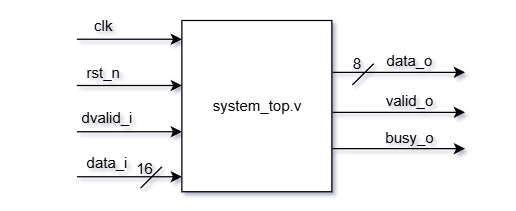
\includegraphics[width=0.8\textwidth]{system_top.png}
    \caption{Sơ đồ khối Top-Level System}
    \label{fig:system_top_block}
\end{figure}

\begin{table}[H]
    \centering
    \caption{Đặc tả giao diện System Top}
    \begin{tabularx}{\textwidth}{|l|c|c|X|}
    \hline
    \textbf{Tên tín hiệu} & \textbf{Độ rộng} & \textbf{Hướng} & \textbf{Mô tả} \\ \hline
    \texttt{clk} & 1 & I & Xung clock hệ thống (Cạnh dương). \\ \hline
    \texttt{rst\_n} & 1 & I & Reset hệ thống (Tích cực thấp). \\ \hline
    \texttt{dvalid\_i} & 1 & I & Tín hiệu báo dữ liệu đầu vào hợp lệ (Sync FIFO WrEn). \\ \hline
    \texttt{data\_i} & 16 & I & Gói dữ liệu đầu vào (16-bit). \\ \hline
    \texttt{data\_o} & 8 & O & Dữ liệu byte đã giải mã (8-bit). \\ \hline
    \texttt{valid\_o} & 1 & O & Tín hiệu báo dữ liệu đầu ra đã sẵn sàng. \\ \hline
    \texttt{busy\_o} & 1 & O & Báo bận khi bộ đệm Sync FIFO đầy. \\ \hline
    \end{tabularx}
\end{table}

\section{Kiến trúc hệ thống và Chi tiết I/O từng khối}
Hệ thống được thiết kế theo luồng dữ liệu Pipeline để tối ưu hóa hiệu năng. Dưới đây là mô tả chi tiết các chân tín hiệu của từng thực thể chức năng.

\subsection{Khối đệm dữ liệu (Sync FIFO)}
Khối này lưu trữ tạm thời dữ liệu 16-bit từ bên ngoài trước khi đưa vào bộ giải mã.

\begin{figure}[H]
    \centering
    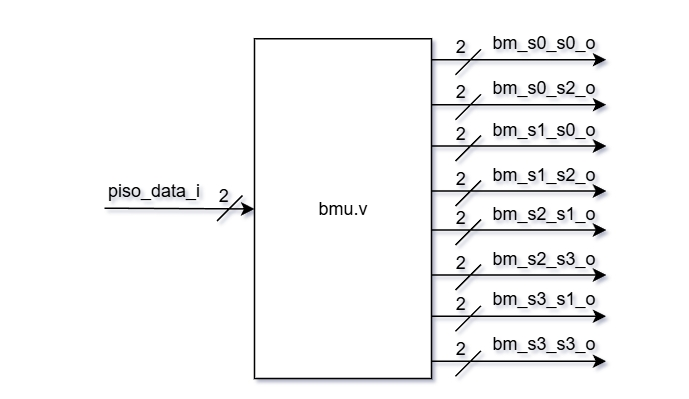
\includegraphics[width=0.8\textwidth]{fifo.png}
    \caption{Sơ đồ khối Sync FIFO}
    \label{fig:fifo_block}
\end{figure}

\paragraph{Mô tả luồng hoạt động:}
Bộ đệm Sync FIFO hoạt động như một bộ nhớ vòng (Circular Buffer) với độ sâu 16 phần tử. Khi tín hiệu ghi (\texttt{wr\_en\_i}) tích cực, dữ liệu đầu vào được lưu vào địa chỉ của con trỏ ghi (\texttt{wr\_ptr}). Khi có yêu cầu đọc (\texttt{rd\_en\_i}), dữ liệu được lấy ra từ địa chỉ của con trỏ đọc (\texttt{rd\_ptr}). Bộ đếm (\texttt{count}) theo dõi số lượng phần tử hiện có để tạo ra các cờ trạng thái \texttt{full\_o} và \texttt{empty\_o}, giúp ngăn chặn hiện tượng tràn (overflow) hoặc đọc rỗng (underflow).


\begin{table}[H]
    \centering
    \caption{Giao diện khối Sync FIFO}
    \begin{tabularx}{\textwidth}{|l|c|c|X|}
    \hline
    \textbf{Tên tín hiệu} & \textbf{Độ rộng} & \textbf{Hướng} & \textbf{Mô tả} \\ \hline
    \texttt{clk} & 1 & I & Xung clock hệ thống. \\ \hline
    \texttt{rst\_n} & 1 & I & Reset hệ thống (Tích cực thấp). \\ \hline
    \texttt{wr\_en\_i} & 1 & I & Lệnh ghi dữ liệu vào Sync FIFO. \\ \hline
    \texttt{wr\_data\_i} & 16 & I & Dữ liệu 16-bit ghi vào. \\ \hline
    \texttt{full\_o} & 1 & O & Cờ báo bộ đệm đã đầy. \\ \hline
    \texttt{rd\_en\_i} & 1 & I & Lệnh đọc dữ liệu ra (từ PISO). \\ \hline
    \texttt{rd\_data\_o} & 16 & O & Dữ liệu 16-bit đọc ra. \\ \hline
    \texttt{empty\_o} & 1 & O & Cờ báo bộ đệm rỗng. \\ \hline
    \end{tabularx}
\end{table}

\subsection{Khối chuyển đổi song song sang nối tiếp (PISO)}
Chuyển đổi gói 16-bit thành các cặp 2-bit (symbol) để nạp vào Viterbi Core.

\begin{figure}[H]
    \centering
    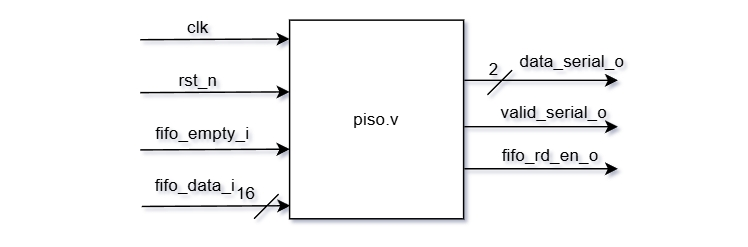
\includegraphics[width=0.8\textwidth]{piso.png}
    \caption{Sơ đồ khối PISO}
    \label{fig:piso_block}
\end{figure}

\paragraph{Mô tả luồng hoạt động:}
PISO được điều khiển bởi một máy trạng thái (FSM) gồm 3 trạng thái:
\begin{itemize}
    \item \textbf{IDLE}: Chờ FIFO báo có dữ liệu (\texttt{!fifo\_empty\_i}). Khi có dữ liệu, chuyển sang chu kỳ đọc.
    \item \textbf{READ\_WAIT}: Kích hoạt tín hiệu đọc gửi tới FIFO (\texttt{fifo\_rd\_en\_o}), nạp 16-bit dữ liệu vào thanh ghi dịch nội bộ.
    \item \textbf{SHIFT}: Thực hiện dịch trái thanh ghi 8 lần. Tại mỗi nhịp, 2 bit cao nhất (MSB) được đẩy ra ngoài (\texttt{data\_serial\_o}) để cung cấp cho Viterbi Core.
\end{itemize}


\begin{table}[H]
    \centering
    \caption{Giao diện khối PISO}
    \begin{tabularx}{\textwidth}{|l|c|c|X|}
    \hline
    \textbf{Tên tín hiệu} & \textbf{Độ rộng} & \textbf{Hướng} & \textbf{Mô tả} \\ \hline
    \texttt{clk} & 1 & I & Xung clock hệ thống. \\ \hline
    \texttt{rst\_n} & 1 & I & Reset hệ thống (Tích cực thấp). \\ \hline
    \texttt{fifo\_data\_i} & 16 & I & Dữ liệu nhận từ Sync FIFO. \\ \hline
    \texttt{fifo\_empty\_i} & 1 & I & Trạng thái rỗng của Sync FIFO. \\ \hline
    \texttt{fifo\_rd\_en\_o} & 1 & O & Lệnh yêu cầu Sync FIFO xuất dữ liệu. \\ \hline
    \texttt{data\_serial\_o} & 2 & O & Cặp bit symbol gửi tới Core. \\ \hline
    \texttt{valid\_serial\_o}& 1 & O & Báo symbol hiện tại hợp lệ. \\ \hline
    \end{tabularx}
\end{table}

\subsection{Khối tính toán chi phí nhánh (BMU)}
Tính khoảng cách Hamming giữa cặp bit nhận được và các nhánh kỳ vọng trong đồ thị lưới.

\begin{figure}[H]
    \centering
    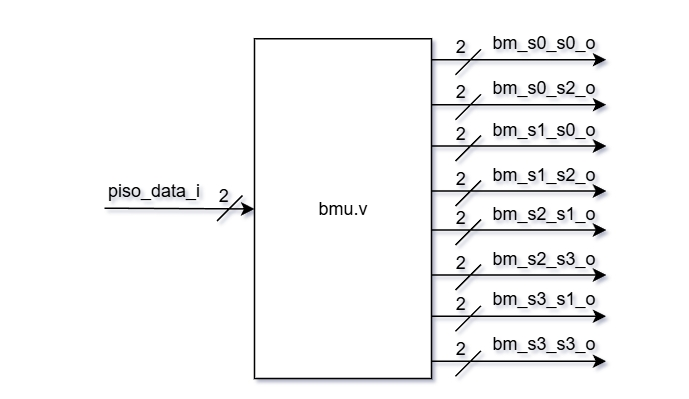
\includegraphics[width=0.8\textwidth]{bmu.png}
    \caption{Sơ đồ khối BMU}
    \label{fig:bmu_block}
\end{figure}

\paragraph{Mô tả luồng hoạt động:}
Khối BMU nhận đầu vào là cặp bit symbol từ PISO và so sánh với 4 cặp nhánh lý thuyết (00, 01, 10, 11). Hàm tính khoảng cách Hamming thực hiện phép XOR từng bit và cộng kết quả để đếm số lượng bit khác nhau. Kết quả là 8 giá trị khoảng cách nhánh (Branch Metrics) được tính toán song song, đại diện cho chi phí để đi từ trạng thái hiện tại đến trạng thái kế tiếp.

\begin{table}[H]
    \centering
    \caption{Giao diện khối BMU}
    \begin{tabularx}{\textwidth}{|l|c|c|X|}
    \hline
    \textbf{Tên tín hiệu} & \textbf{Độ rộng} & \textbf{Hướng} & \textbf{Mô tả} \\ \hline
    \texttt{piso\_data\_i} & 2 & I & Dữ liệu 2-bit từ PISO. \\ \hline
    \texttt{bm\_s0\_s0\_o} & 2 & O & Chi phí nhánh từ S0 đến S0. \\ \hline
    \texttt{bm\_s0\_s2\_o} & 2 & O & Chi phí nhánh từ S0 đến S2. \\ \hline
    \texttt{bm\_s1\_s0\_o} & 2 & O & Chi phí nhánh từ S1 đến S0. \\ \hline
    \texttt{bm\_s1\_s2\_o} & 2 & O & Chi phí nhánh từ S1 đến S2. \\ \hline
    \texttt{bm\_s2\_s1\_o} & 2 & O & Chi phí nhánh từ S2 đến S1. \\ \hline
    \texttt{bm\_s2\_s3\_o} & 2 & O & Chi phí nhánh từ S2 đến S3. \\ \hline
    \texttt{bm\_s3\_s1\_o} & 2 & O & Chi phí nhánh từ S3 đến S1. \\ \hline
    \texttt{bm\_s3\_s3\_o} & 2 & O & Chi phí nhánh từ S3 đến S3. \\ \hline
    \end{tabularx}
\end{table}

\subsection{Khối Cộng - So sánh - Chọn (ACSU)}
Cập nhật Path Metric cho 4 trạng thái và đưa ra quyết định chọn đường dẫn (Survivor Path).

\begin{figure}[H]
    \centering
    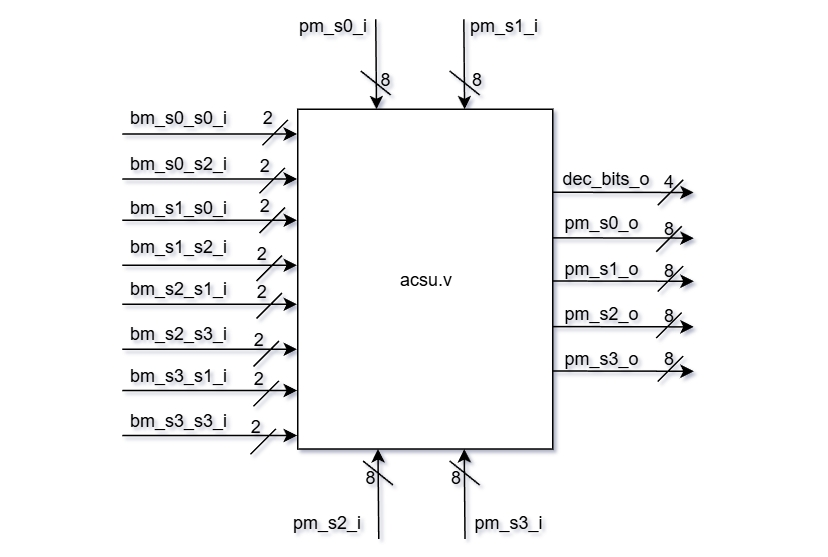
\includegraphics[width=0.8\textwidth]{acsu.png}
    \caption{Sơ đồ khối ACSU}
    \label{fig:acsu_block}
\end{figure}

\paragraph{Mô tả luồng hoạt động:}
Khối ACSU nhận 8 Metric nhánh từ BMU và 4 Metric đường dẫn từ PMU. Với mỗi trạng thái đích, ACSU tính toán hai tổng chi phí tiềm năng (Candidate Path Metrics) từ hai trạng thái nguồn. Bộ so sánh xác định đường dẫn có chi phí nhỏ hơn và cập nhật giá trị đó làm Path Metric mới (\texttt{pm\_new\_sX}). Đồng thời, bit quyết định (0 hoặc 1) tương ứng với nhánh được chọn sẽ được gửi tới khối TBU để lưu lại lịch sử.

\begin{table}[H]
    \centering
    \caption{Giao diện khối ACSU}
    \begin{tabularx}{\textwidth}{|l|c|c|X|}
    \hline
    \textbf{Tên tín hiệu} & \textbf{Độ rộng} & \textbf{Hướng} & \textbf{Mô tả} \\ \hline
    \texttt{bm\_s0\_s0\_i} & 2 & I & Chi phí nhánh từ S0 đến S0. \\ \hline
    \texttt{bm\_s0\_s2\_i} & 2 & I & Chi phí nhánh từ S0 đến S2. \\ \hline
    \texttt{bm\_s1\_s0\_i} & 2 & I & Chi phí nhánh từ S1 đến S0. \\ \hline
    \texttt{bm\_s1\_s2\_i} & 2 & I & Chi phí nhánh từ S1 đến S2. \\ \hline
    \texttt{bm\_s2\_s1\_i} & 2 & I & Chi phí nhánh từ S2 đến S1. \\ \hline
    \texttt{bm\_s2\_s3\_i} & 2 & I & Chi phí nhánh từ S2 đến S3. \\ \hline
    \texttt{bm\_s3\_s1\_i} & 2 & I & Chi phí nhánh từ S3 đến S1. \\ \hline
    \texttt{bm\_s3\_s3\_i} & 2 & I & Chi phí nhánh từ S3 đến S3. \\ \hline
    \texttt{pm\_s0\_i} & 8 & I & Chi phí đường đi hiện tại của S0. \\ \hline
    \texttt{pm\_s1\_i} & 8 & I & Chi phí đường đi hiện tại của S1. \\ \hline
    \texttt{pm\_s2\_i} & 8 & I & Chi phí đường đi hiện tại của S2. \\ \hline
    \texttt{pm\_s3\_i} & 8 & I & Chi phí đường đi hiện tại của S3. \\ \hline
    \texttt{pm\_s0\_o} & 8 & O & Chi phí đường đi mới của S0. \\ \hline
    \texttt{pm\_s1\_o} & 8 & O & Chi phí đường đi mới của S1. \\ \hline
    \texttt{pm\_s2\_o} & 8 & O & Chi phí đường đi mới của S2. \\ \hline
    \texttt{pm\_s3\_o} & 8 & O & Chi phí đường đi mới của S3. \\ \hline
    \texttt{dec\_bits\_o} & 4 & O & 4 bit quyết định chọn nhánh (1 bit mỗi trạng thái). \\ \hline
    \end{tabularx}
\end{table}

\subsection{Khối quản lý Path Metric (PMU)}
Lưu trữ và phản hồi chi phí tích lũy của các trạng thái.

\begin{figure}[H]
    \centering
    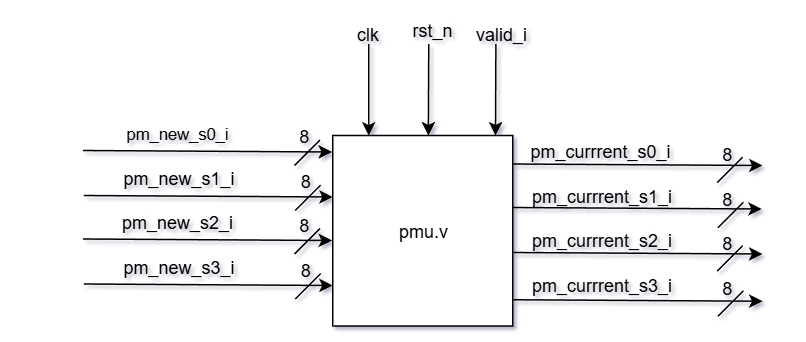
\includegraphics[width=0.8\textwidth]{pmu.png}
    \caption{Sơ đồ khối PMU}
    \label{fig:pmu_block}
\end{figure}

\paragraph{Mô tả luồng hoạt động:}
PMU đóng vai trò là bộ nhớ trạng thái của thuật toán Viterbi. Khi có tín hiệu kích hoạt (\texttt{valid\_i}), PMU cập nhật 4 thanh ghi lưu trữ giá trị Metric mới nhất nhận được từ ACSU. Khi Reset, trạng thái $S_0$ được khởi tạo giá trị 0, trong khi các trạng thái khác được gán giá trị tối đa (255) để đảm bảo thuật toán luôn bắt đầu tìm kiếm từ trạng thái $S_0$.


\begin{table}[H]
    \centering
    \caption{Giao diện khối PMU}
    \begin{tabularx}{\textwidth}{|l|c|c|X|}
    \hline
    \textbf{Tên tín hiệu} & \textbf{Độ rộng} & \textbf{Hướng} & \textbf{Mô tả} \\ \hline
    \texttt{clk} & 1 & I & Xung clock hệ thống. \\ \hline
    \texttt{rst\_n} & 1 & I & Reset hệ thống (Tích cực thấp). \\ \hline
    \texttt{valid\_i} & 1 & I & Cho phép cập nhật giá trị mới. \\ \hline
    \texttt{pm\_new\_s0\_i} & 8 & I & Giá trị mới từ ACSU cho S0. \\ \hline
    \texttt{pm\_new\_s1\_i} & 8 & I & Giá trị mới từ ACSU cho S1. \\ \hline
    \texttt{pm\_new\_s2\_i} & 8 & I & Giá trị mới từ ACSU cho S2. \\ \hline
    \texttt{pm\_new\_s3\_i} & 8 & I & Giá trị mới từ ACSU cho S3. \\ \hline
    \texttt{pm\_current\_s0\_o} & 8 & O & Giá trị hiện tại của S0 gửi ACSU. \\ \hline
    \texttt{pm\_current\_s1\_o} & 8 & O & Giá trị hiện tại của S1 gửi ACSU. \\ \hline
    \texttt{pm\_current\_s2\_o} & 8 & O & Giá trị hiện tại của S2 gửi ACSU. \\ \hline
    \texttt{pm\_current\_s3\_o} & 8 & O & Giá trị hiện tại của S3 gửi ACSU. \\ \hline
    \end{tabularx}
\end{table}

\subsection{Khối truy vết Survivor Memory (TBU - Register Exchange)}
Thực hiện kỹ thuật Register Exchange để khôi phục bit gốc từ các bit quyết định.

\begin{figure}[H]
    \centering
    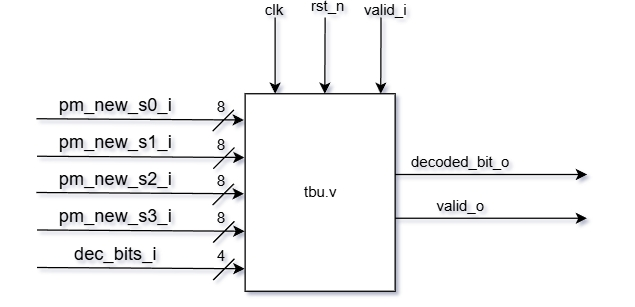
\includegraphics[width=0.8\textwidth]{tbu.png}
    \caption{Sơ đồ khối TBU}
    \label{fig:tbu_block}
\end{figure}

\paragraph{Mô tả luồng hoạt động:}
TBU quản lý 4 thanh ghi lịch sử 15-bit cho 4 trạng thái. Tại mỗi chu kỳ clock, dựa trên 4 bit quyết định từ ACSU, nội dung của các thanh ghi này được cập nhật theo quy tắc Register Exchange: Thanh ghi của trạng thái $S_k$ sẽ nhận giá trị từ thanh ghi của trạng thái nguồn đã đi tới nó, cộng thêm bit quyết định mới. Sau khi pipeline đầy, bộ so sánh so sánh 4 giá trị Path Metric hiện tại để tìm trạng thái tối ưu nhất, và bit cũ nhất (MSB) trong thanh ghi lịch sử của trạng thái đó sẽ được chọn làm bit đầu ra (\texttt{decoded\_bit\_o}).


\begin{table}[H]
    \centering
    \caption{Giao diện khối TBU}
    \begin{tabularx}{\textwidth}{|l|c|c|X|}
    \hline
    \textbf{Tên tín hiệu} & \textbf{Độ rộng} & \textbf{Hướng} & \textbf{Mô tả} \\ \hline
    \texttt{clk} & 1 & I & Xung clock hệ thống. \\ \hline
    \texttt{rst\_n} & 1 & I & Reset hệ thống (Tích cực thấp). \\ \hline
    \texttt{valid\_i} & 1 & I & Tín hiệu cho phép cập nhật. \\ \hline
    \texttt{dec\_bits\_i} & 4 & I & Các bit quyết định từ ACSU. \\ \hline
    \texttt{pm\_new\_s0\_i} & 8 & I & Chi phí đường dẫn mới của S0 (để so sánh). \\ \hline
    \texttt{pm\_new\_s1\_i} & 8 & I & Chi phí đường dẫn mới của S1 (để so sánh). \\ \hline
    \texttt{pm\_new\_s2\_i} & 8 & I & Chi phí đường dẫn mới của S2 (để so sánh). \\ \hline
    \texttt{pm\_new\_s3\_i} & 8 & I & Chi phí đường dẫn mới của S3 (để so sánh). \\ \hline
    \texttt{decoded\_bit\_o}& 1 & O & Bit dữ liệu đã giải mã thành công. \\ \hline
    \texttt{valid\_o} & 1 & O & Báo bit giải mã hợp lệ. \\ \hline
    \end{tabularx}
\end{table}

\subsection{Khối chuyển đổi nối tiếp sang song song (SIPO)}
Gom các bit đơn lẻ từ TBU thành byte 8-bit hoàn chỉnh trước khi xuất ra ngoài hệ thống.

\begin{figure}[H]
    \centering
    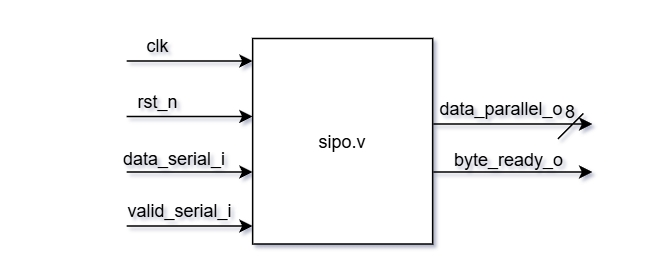
\includegraphics[width=0.8\textwidth]{sipo.png}
    \caption{Sơ đồ khối SIPO}
    \label{fig:sipo_block}
\end{figure}

\paragraph{Mô tả luồng hoạt động:}
Khối SIPO gom các bit đơn lẻ được giải mã từ TBU thành byte dữ liệu hoàn chỉnh. Mỗi khi nhận một bit hợp lệ (\texttt{valid\_serial\_i}), bit này được dịch vào thanh ghi đệm từ vị trí MSB. Bộ đếm theo dõi số lượng bit đã nhận; khi đếm đủ 8 bit, tín hiệu \texttt{byte\_ready\_o} được kích hoạt, báo hiệu một byte dữ liệu (\texttt{data\_parallel\_o}) đã sẵn sàng để xuất ra output.


\begin{table}[H]
    \centering
    \caption{Giao diện khối SIPO}
    \begin{tabularx}{\textwidth}{|l|c|c|X|}
    \hline
    \textbf{Tên tín hiệu} & \textbf{Độ rộng} & \textbf{Hướng} & \textbf{Mô tả} \\ \hline
    \texttt{clk} & 1 & I & Xung clock hệ thống. \\ \hline
    \texttt{rst\_n} & 1 & I & Reset hệ thống (Tích cực thấp). \\ \hline
    \texttt{data\_serial\_i} & 1 & I & Bit nhận từ TBU. \\ \hline
    \texttt{valid\_serial\_i}& 1 & I & Cờ báo bit đầu vào hợp lệ. \\ \hline
    \texttt{data\_parallel\_o}& 8 & O & Dữ liệu byte hoàn chỉnh. \\ \hline
    \texttt{byte\_ready\_o} & 1 & O & Báo hiệu đã đủ 8 bit (Byte Valid). \\ \hline
    \end{tabularx}
\end{table}

\section{Triển khai RTL (RTL Implementation)}
Mã nguồn RTL được viết bằng Verilog HDL.
Trước khi đi vào chi tiết, sơ đồ khối hệ thống (Hình \ref{fig:system_block}) và lưu đồ thuật toán (Hình \ref{fig:algo_flow}) minh họa luồng xử lý tổng quan.

\begin{figure}[H]
    \centering
    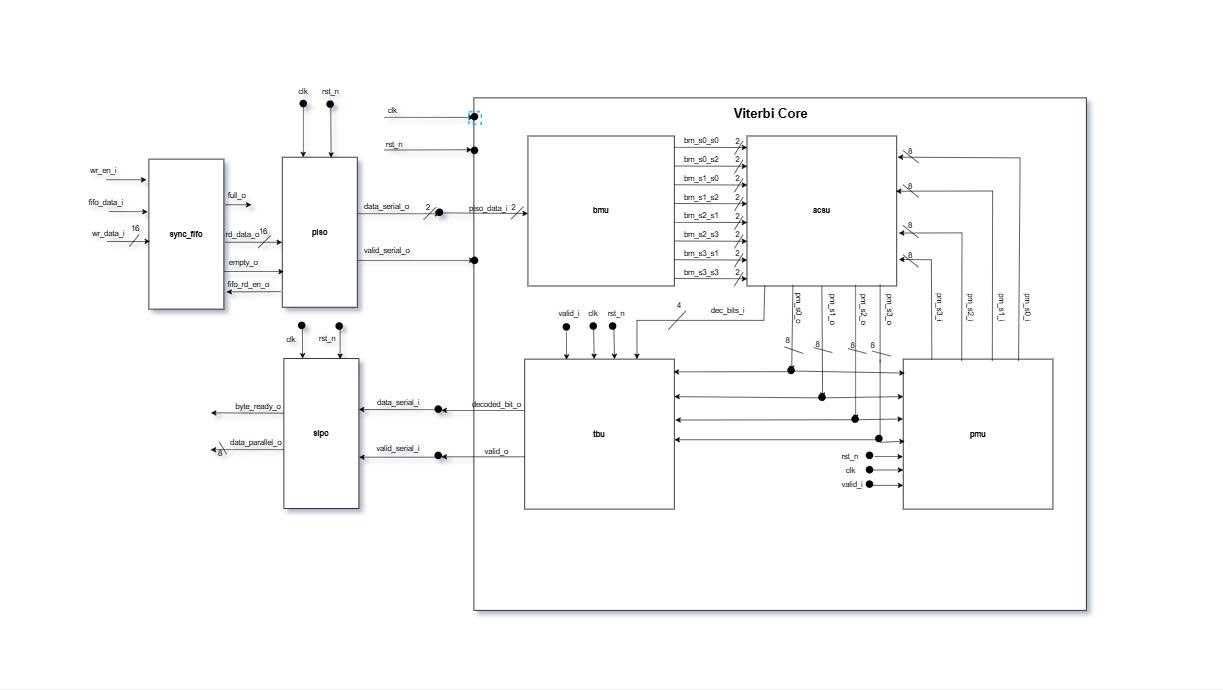
\includegraphics[width=1.1\textwidth]{sdk.jpg}
    \caption{Sơ đồ khối chi tiết hệ thống Viterbi Decoder SoC}
    \label{fig:system_block}
\end{figure}

Lưu đồ thuật toán điều khiển luồng dữ liệu:

\begin{figure}[H]
    \centering
    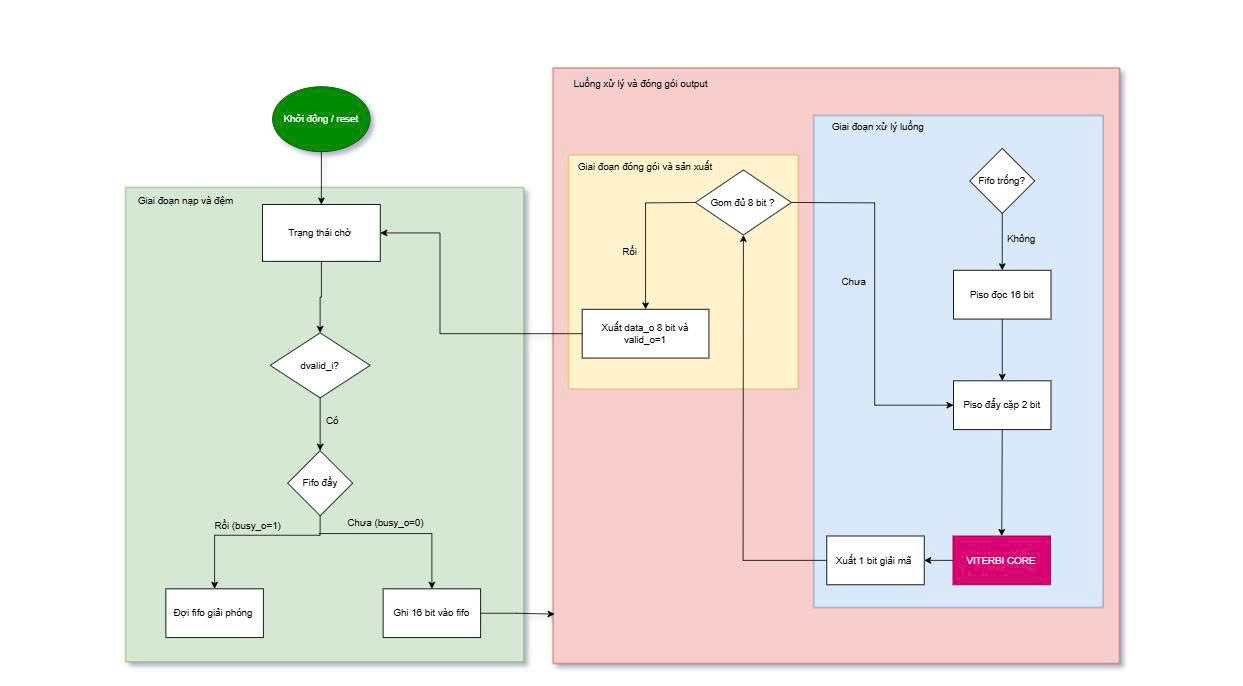
\includegraphics[width=1.1\textwidth]{ldtt.jpg}
    \caption{Lưu đồ thuật toán điều khiển luồng dữ liệu hệ thống}
    \label{fig:algo_flow}
\end{figure}
\newpage

Thay vì sử dụng bộ nhớ RAM để lưu vết và quay lui (Traceback) gây độ trễ lớn, nhóm sử dụng kỹ thuật \textbf{Register Exchange (RE)} trong khối TBU. 

Mỗi trạng thái ($S_0, S_1, S_2, S_3$) quản lý một thanh ghi dịch lịch sử dài 15 bit.
\begin{lstlisting}[language=Verilog, caption=Cơ chế Register Exchange trong TBU]
// Update logic example for state S0
if (dec_bits_i[0] == 0) 
    history_s0 <= {history_s0[TBL-2:0], 1'b0}; // Select path from previous S0
else                    
    history_s0 <= {history_s1[TBL-2:0], 1'b0}; // Select path from previous S1
\end{lstlisting}

Nhờ cơ chế này, sau khi pipeline được điền đầy (15 chu kỳ), đầu ra dữ liệu là liên tục (streaming) với năng suất (throughput) cao nhất (1 bit/cycle).

% ====================================================================
% CHƯƠNG 3
% ====================================================================
\chapter{KIỂM TRA CHỨC NĂNG MẠCH}

\section{Môi trường kiểm chứng (Testbench Environment)}
Môi trường kiểm tra được xây dựng trong file \texttt{tb\_system\_top.sv} với các thành phần:
\begin{itemize}
    \item \textbf{Generator}: Tạo ngẫu nhiên 1025 gói dữ liệu 16-bit.
    \item \textbf{Driver}: Đưa dữ liệu vào hệ thống qua giao thức bắt tay (valid/busy).
    \item \textbf{Monitor}: Thu thập dữ liệu đầu ra \texttt{data\_o}.
    \item \textbf{Scoreboard}: So sánh kết quả mô phỏng với "Golden Model" (mô hình chuẩn).
\end{itemize}

\section{Kết quả mô phỏng (Simulation Results)}
Dưới đây là kết quả mô phỏng chi tiết cho từng khối chức năng (Unit Level) và toàn hệ thống (System Level). Các hình ảnh bao gồm log dữ liệu và giản đồ sóng xác nhận hoạt động chính xác của thiết kế.

% --- FIFO ---
\subsection{Khối đệm dữ liệu (Sync FIFO)}
Bảng dưới đây mô tả các kịch bản kiểm thử được thực hiện cho khối Sync FIFO:

\begin{longtable}{|l|l|p{4cm}|p{4cm}|l|}
\hline
\textbf{ID} & \textbf{Tên Kịch Bản} & \textbf{Hành động} & \textbf{Kỳ vọng} & \textbf{Kết quả} \\
\hline
\endhead
TC\_01 & Reset \& Init & Kích hoạt rst\_n xuống 0 rồi lên 1. & empty\_o=1, full\_o=0. & PASS \\
\hline
TC\_02 & Write until Full & Ghi liên tục 16 phần tử. & full\_o chuyển lên 1. & PASS \\
\hline
TC\_03 & Read until Empty & Đọc liên tục 16 phần tử. & empty\_o chuyển lên 1, dữ liệu khớp. & PASS \\
\hline
TC\_04 & Data Integrity & Lặp Ghi đầy - Đọc rỗng 5 vòng. & Dữ liệu khớp mỗi vòng. & PASS \\
\hline
TC\_05 & Timing Check & Kiểm tra độ trễ dữ liệu ra. & Dữ liệu ổn định sau cạnh clock. & PASS \\
\hline
\caption{Các kịch bản kiểm thử khối Sync FIFO}
\end{longtable}

\begin{figure}[H]
    \centering
    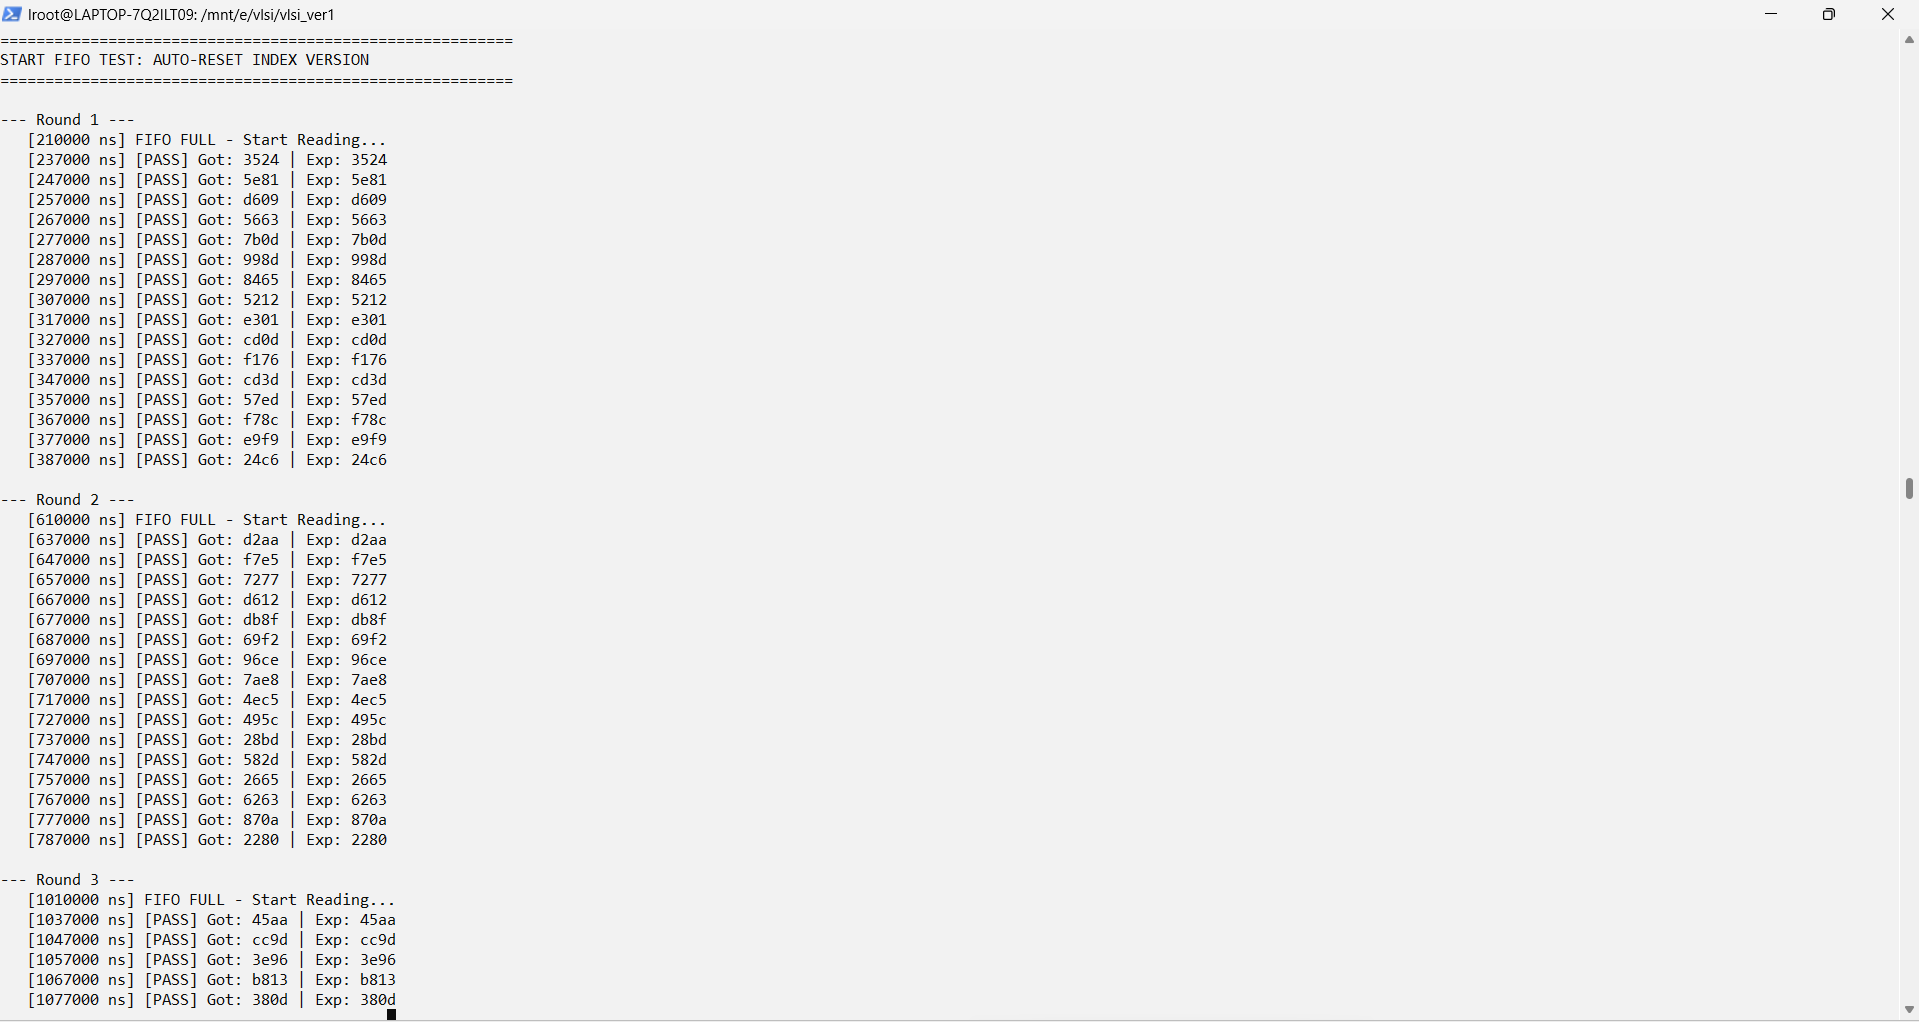
\includegraphics[width=1.0\textwidth]{fifo_log_part1.png}
    \caption{Log mô phỏng Sync FIFO - Phần 1}
\end{figure}
\begin{figure}[H]
    \centering
    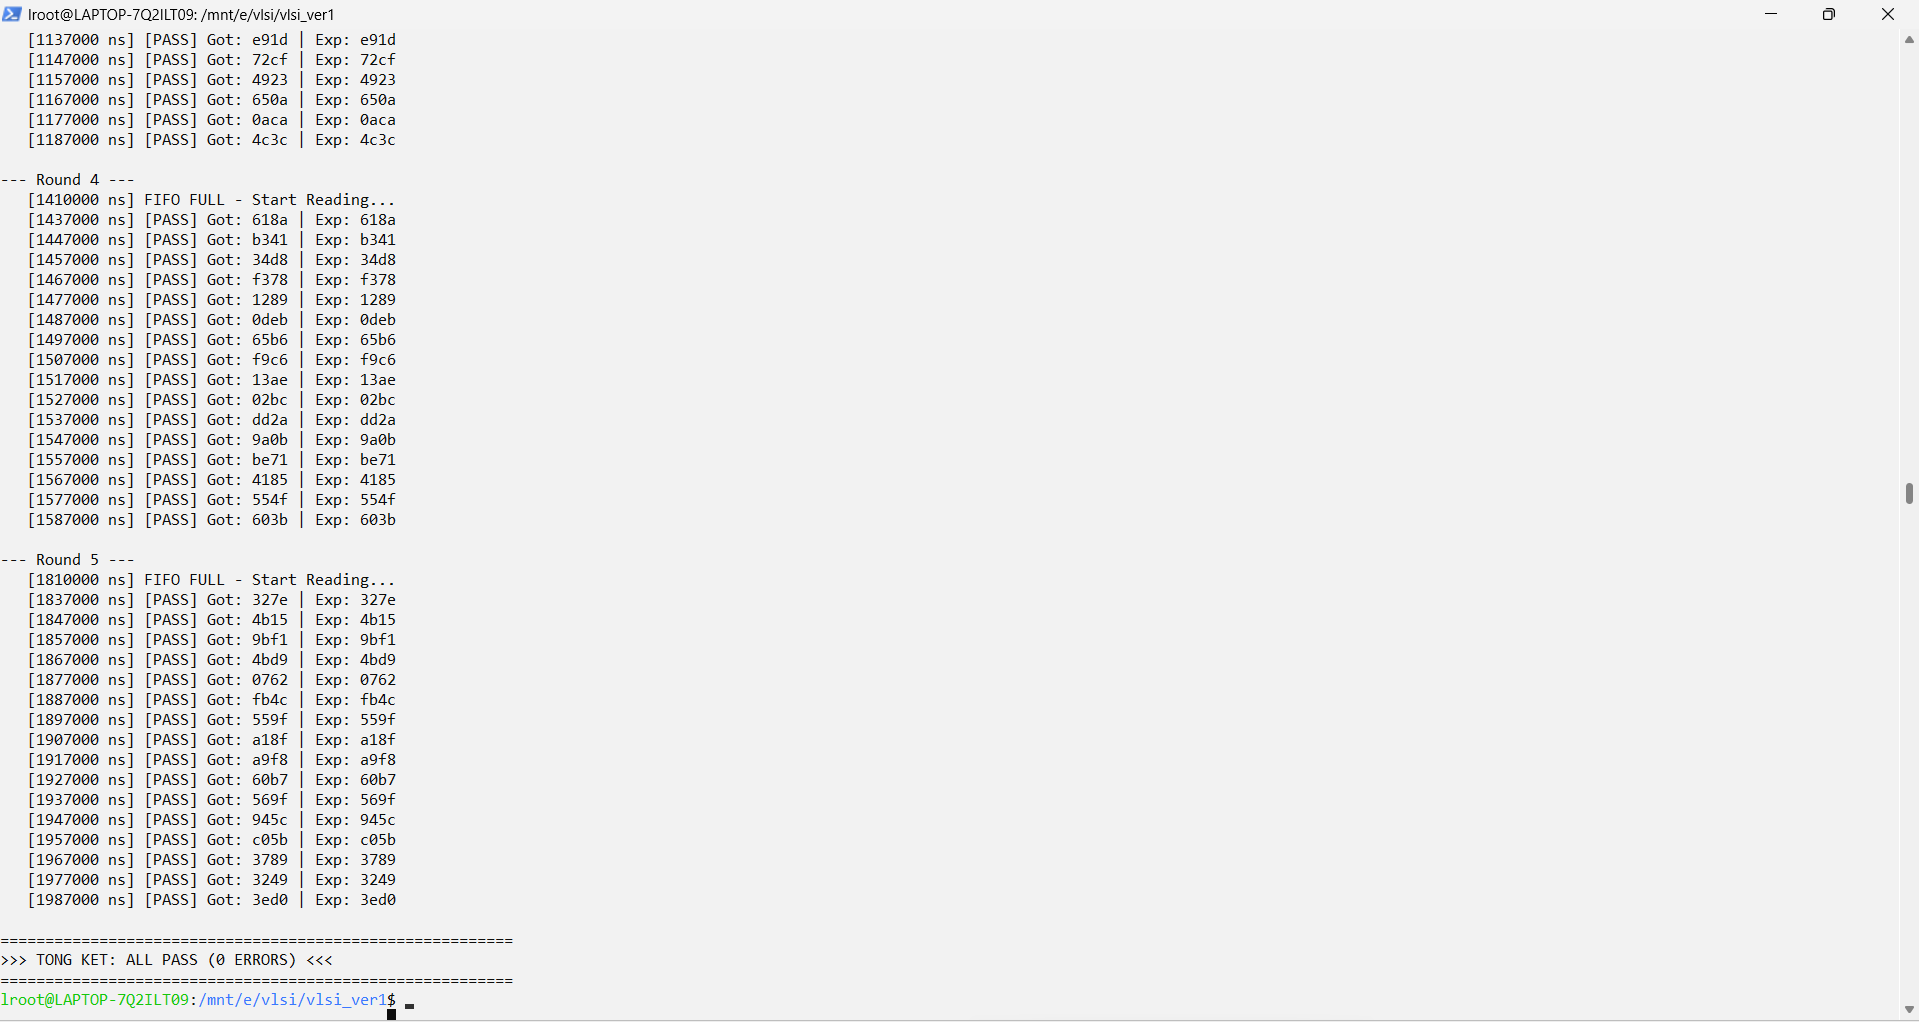
\includegraphics[width=1.0\textwidth]{fifo_log_part2.png}
    \caption{Log mô phỏng Sync FIFO - Phần 2}
\end{figure}
\begin{figure}[H]
    \centering
    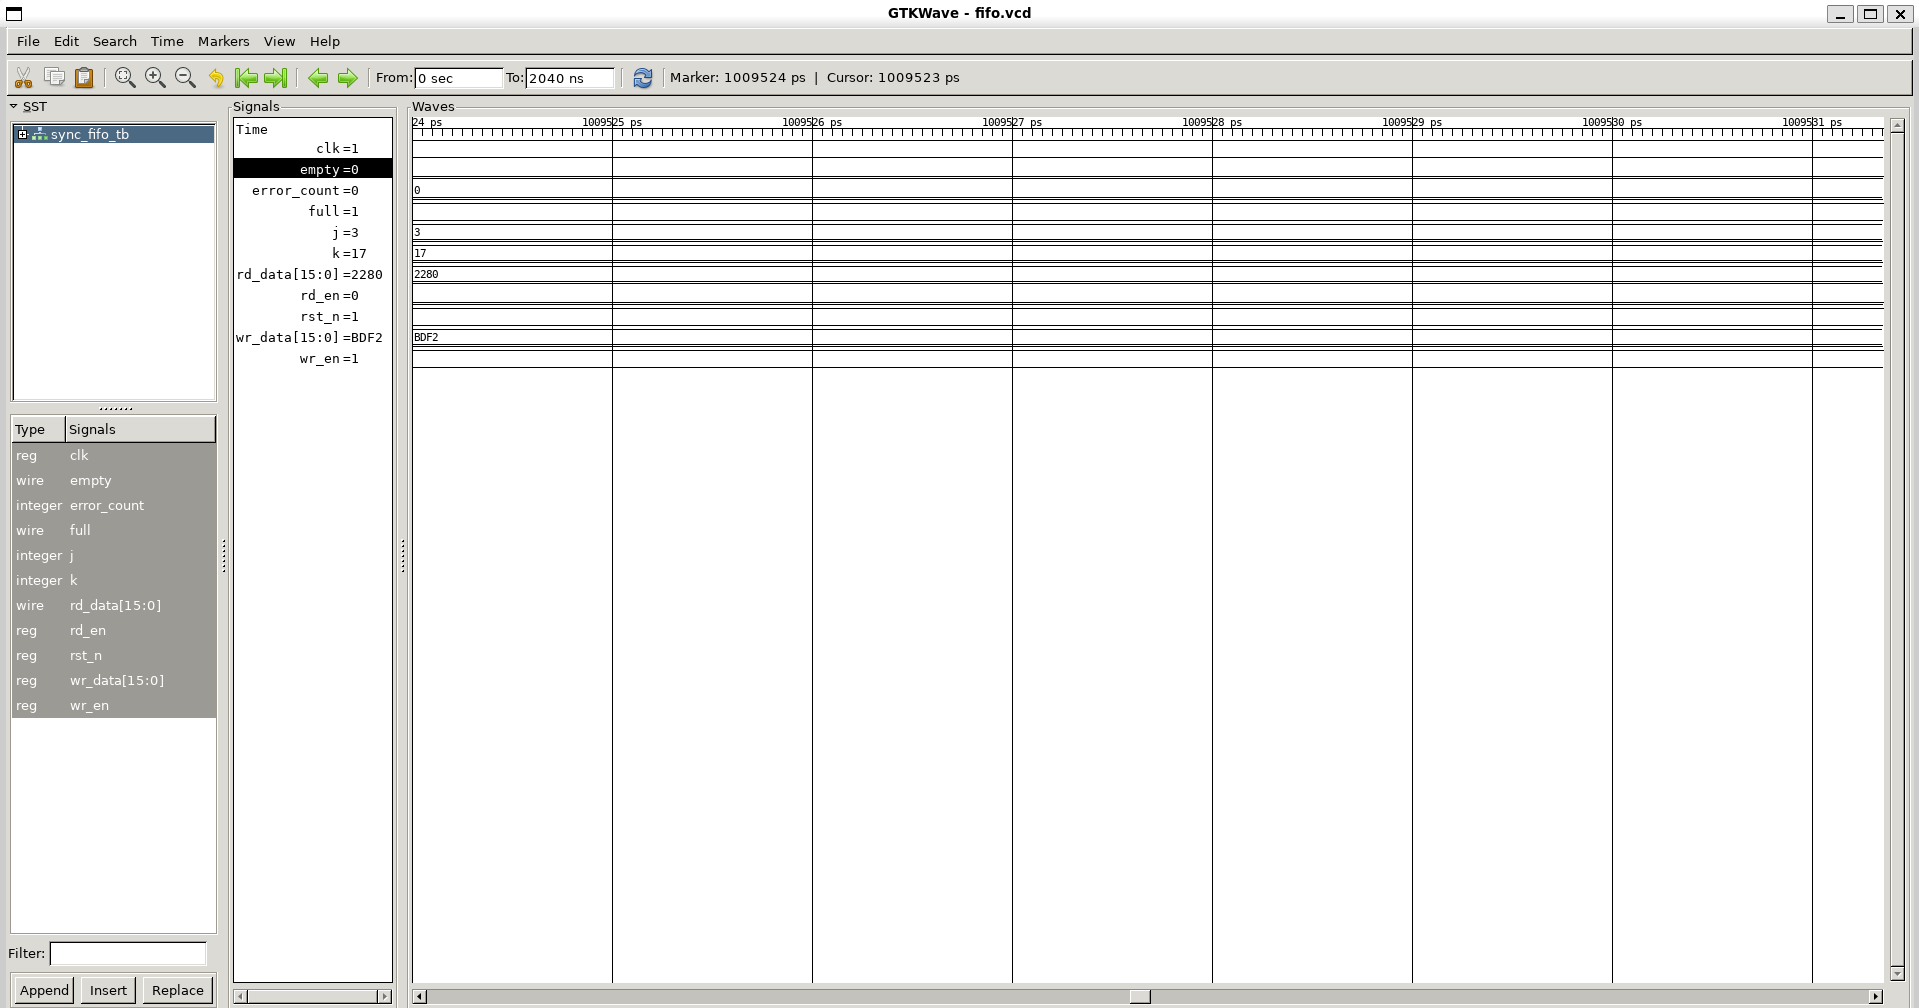
\includegraphics[width=1.0\textwidth]{fifo_wave.png}
    \caption{Giản đồ sóng tín hiệu Sync FIFO}
\end{figure}

% --- PISO ---
\subsection{Khối chuyển đổi song song sang nối tiếp (PISO)}
Bảng dưới đây mô tả các kịch bản kiểm thử được thực hiện cho khối PISO:

\begin{longtable}{|l|l|p{3cm}|p{4cm}|l|}
\hline
\textbf{ID} & \textbf{Tên Kịch Bản} & \textbf{Dữ liệu vào} & \textbf{Kỳ vọng} & \textbf{Kết quả} \\
\hline
\endhead
TC\_01 & Alternating (0xAAAA) & 16'hAAAA & Xuất 8 cặp: 10,10,10... & PASS \\
\hline
TC\_02 & Inverse (0x5555) & 16'h5555 & Xuất 8 cặp: 01,01,01... & PASS \\
\hline
TC\_03 & All Ones (0xFFFF) & 16'hFFFF & Xuất 8 cặp: 11,11,11... & PASS \\
\hline
TC\_04 & All Zeros (0x0000) & 16'h0000 & Xuất 8 cặp: 00,00,00... & PASS \\
\hline
TC\_05 & Random Stress & Ngẫu nhiên & Dữ liệu khớp sau 5 vòng. & PASS \\
\hline
\caption{Các kịch bản kiểm thử khối PISO}
\end{longtable}

\begin{figure}[H]
    \centering
    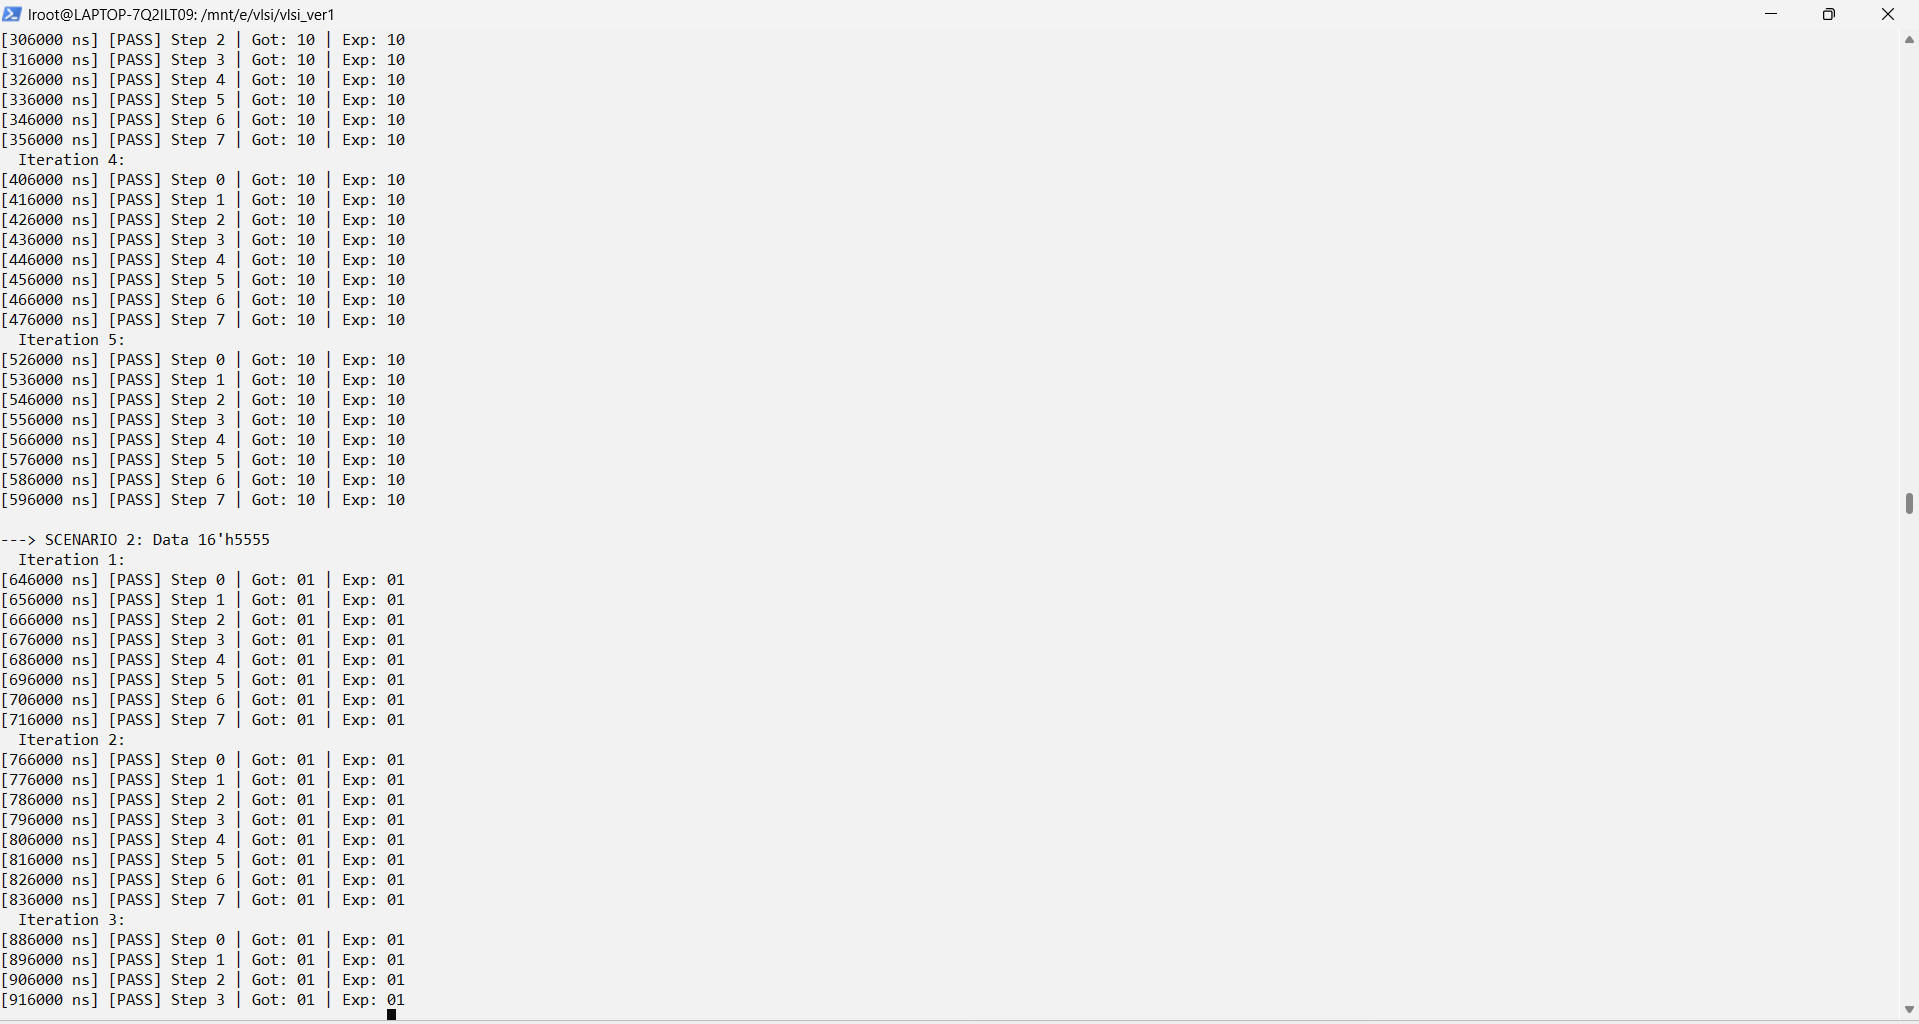
\includegraphics[width=1.0\textwidth]{piso_log_part1.png}
    \caption{Log mô phỏng PISO - Phần 1}
\end{figure}
\begin{figure}[H]
    \centering
    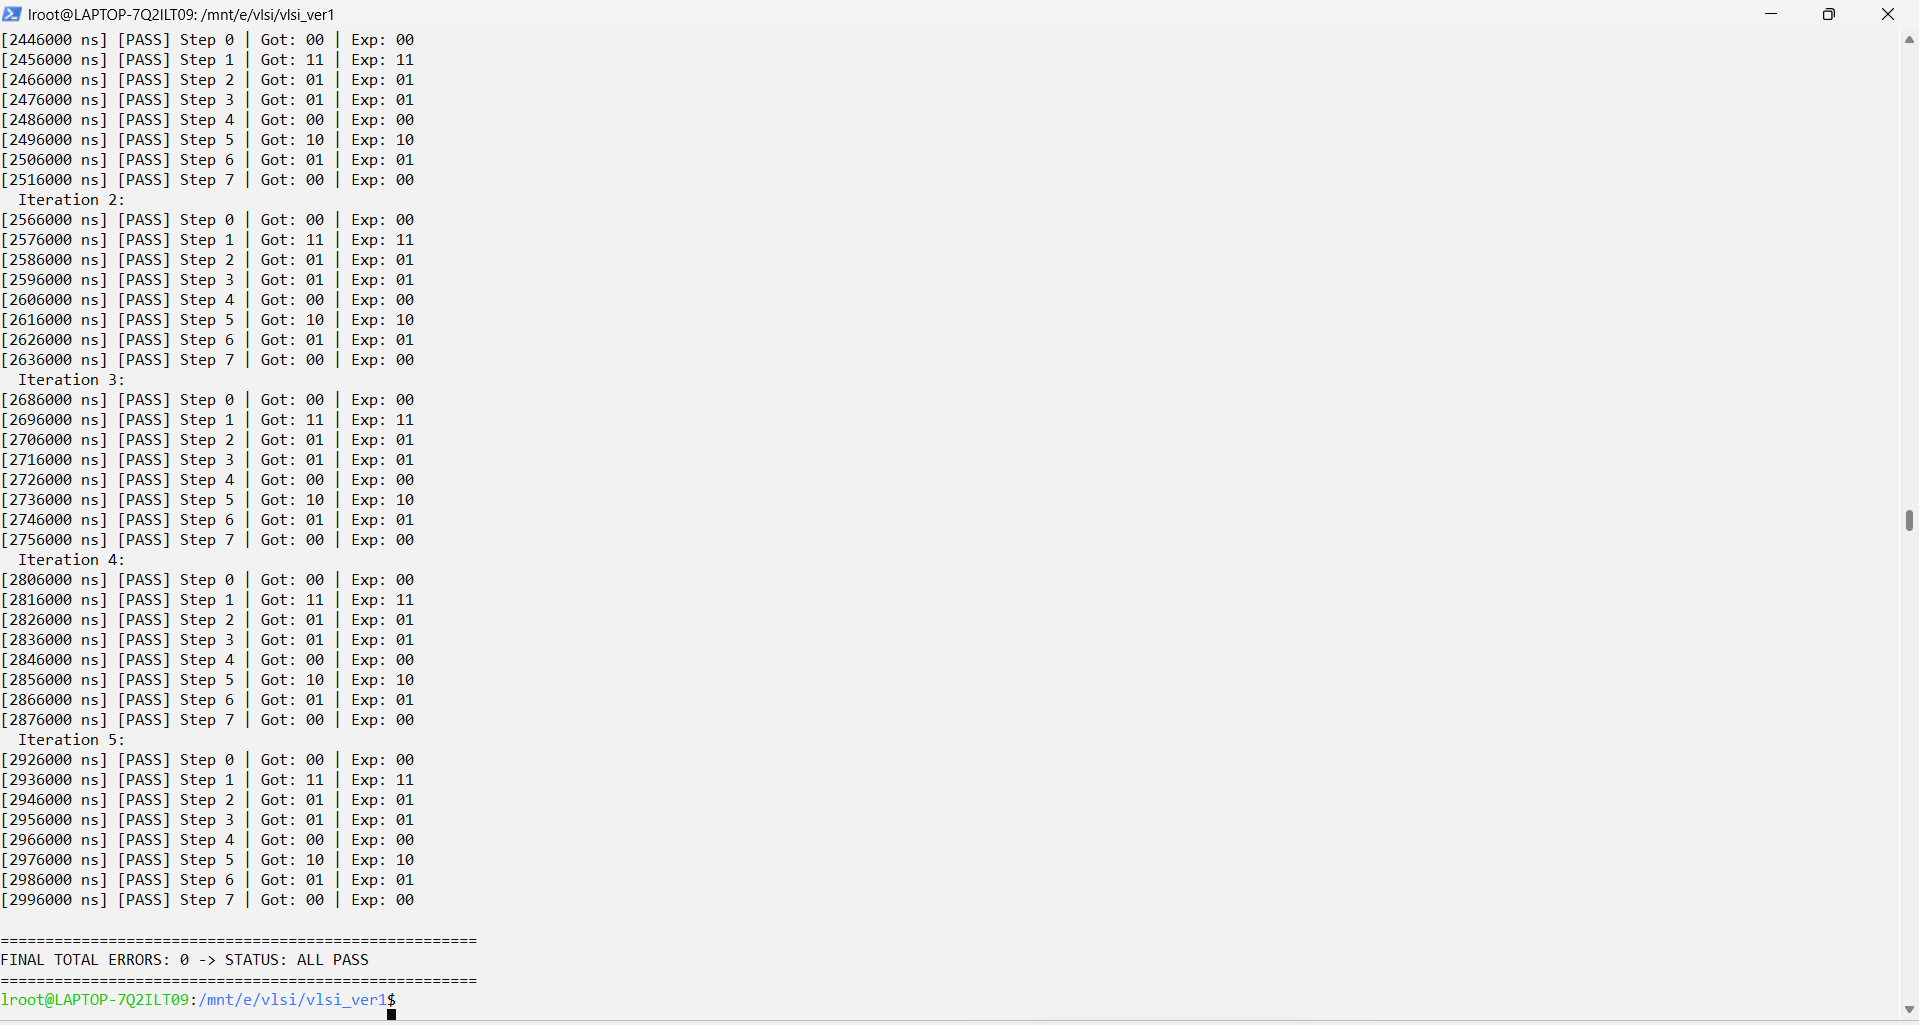
\includegraphics[width=1.0\textwidth]{piso_log_part2.png}
    \caption{Log mô phỏng PISO - Phần 2}
\end{figure}
\begin{figure}[H]
    \centering
    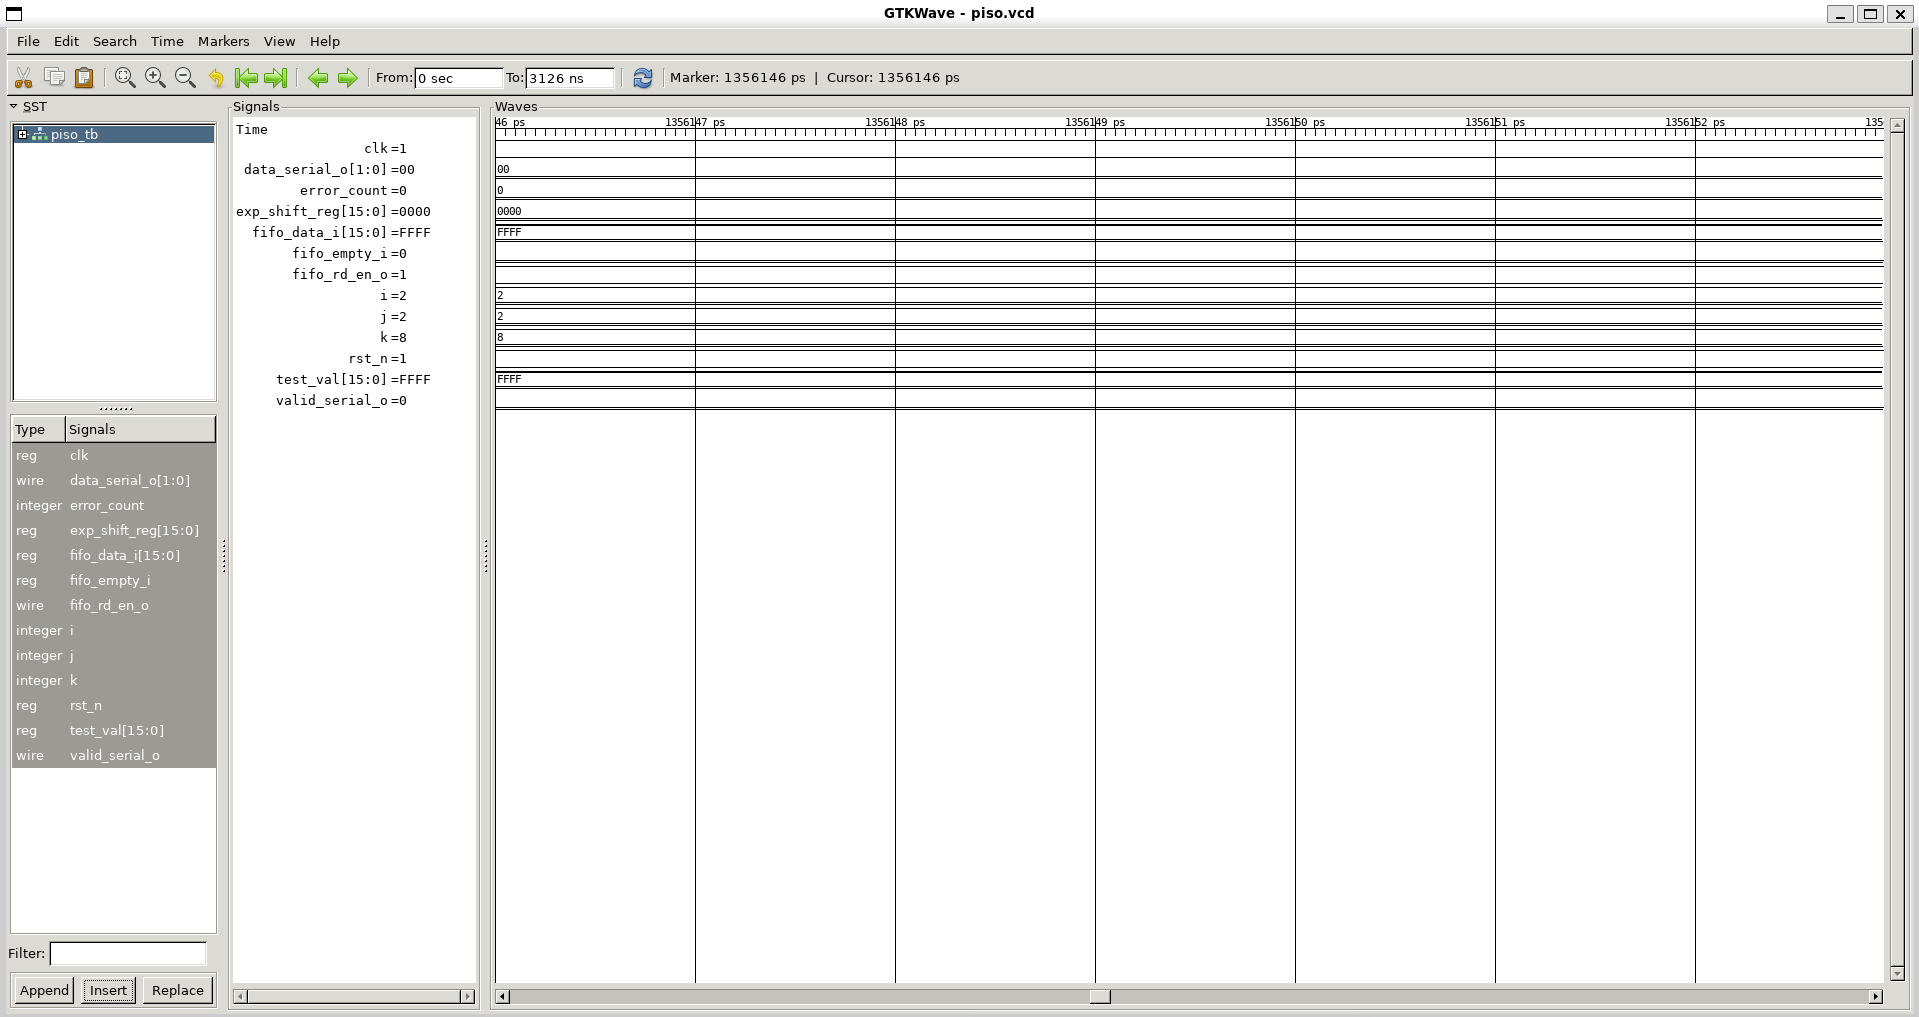
\includegraphics[width=1.0\textwidth]{piso_wave.png}
    \caption{Giản đồ sóng tín hiệu PISO}
\end{figure}

% --- BMU ---
\subsection{Khối tính toán nhánh (BMU)}
Bảng dưới đây mô tả các kịch bản kiểm thử được thực hiện cho khối BMU:

\begin{longtable}{|l|l|l|p{5cm}|l|}
\hline
\textbf{ID} & \textbf{Tên Kịch Bản} & \textbf{Input} & \textbf{Kỳ vọng (Branch Metrics)} & \textbf{Kết quả} \\
\hline
\endhead
TC\_01 & Ideal Case (00) & 2'b00 & S0-S0:0, S1-S2:0, S0-S2:2, S1-S0:2 & PASS \\
\hline
TC\_02 & Inverse Case (11) & 2'b11 & S0-S0:2, S1-S2:2, S0-S2:0, S1-S0:0 & PASS \\
\hline
TC\_03 & Single Bit (01) & 2'b01 & Nhánh kỳ vọng 01/10: 0 hoặc 1 & PASS \\
\hline
TC\_04 & Single Bit (10) & 2'b10 & Tương tự TC\_03, đảo vị trí & PASS \\
\hline
TC\_05 & Random Stress & Ngẫu nhiên & Ngõ ra thay đổi tức thời & PASS \\
\hline
\caption{Các kịch bản kiểm thử khối BMU}
\end{longtable}

\begin{figure}[H]
    \centering
    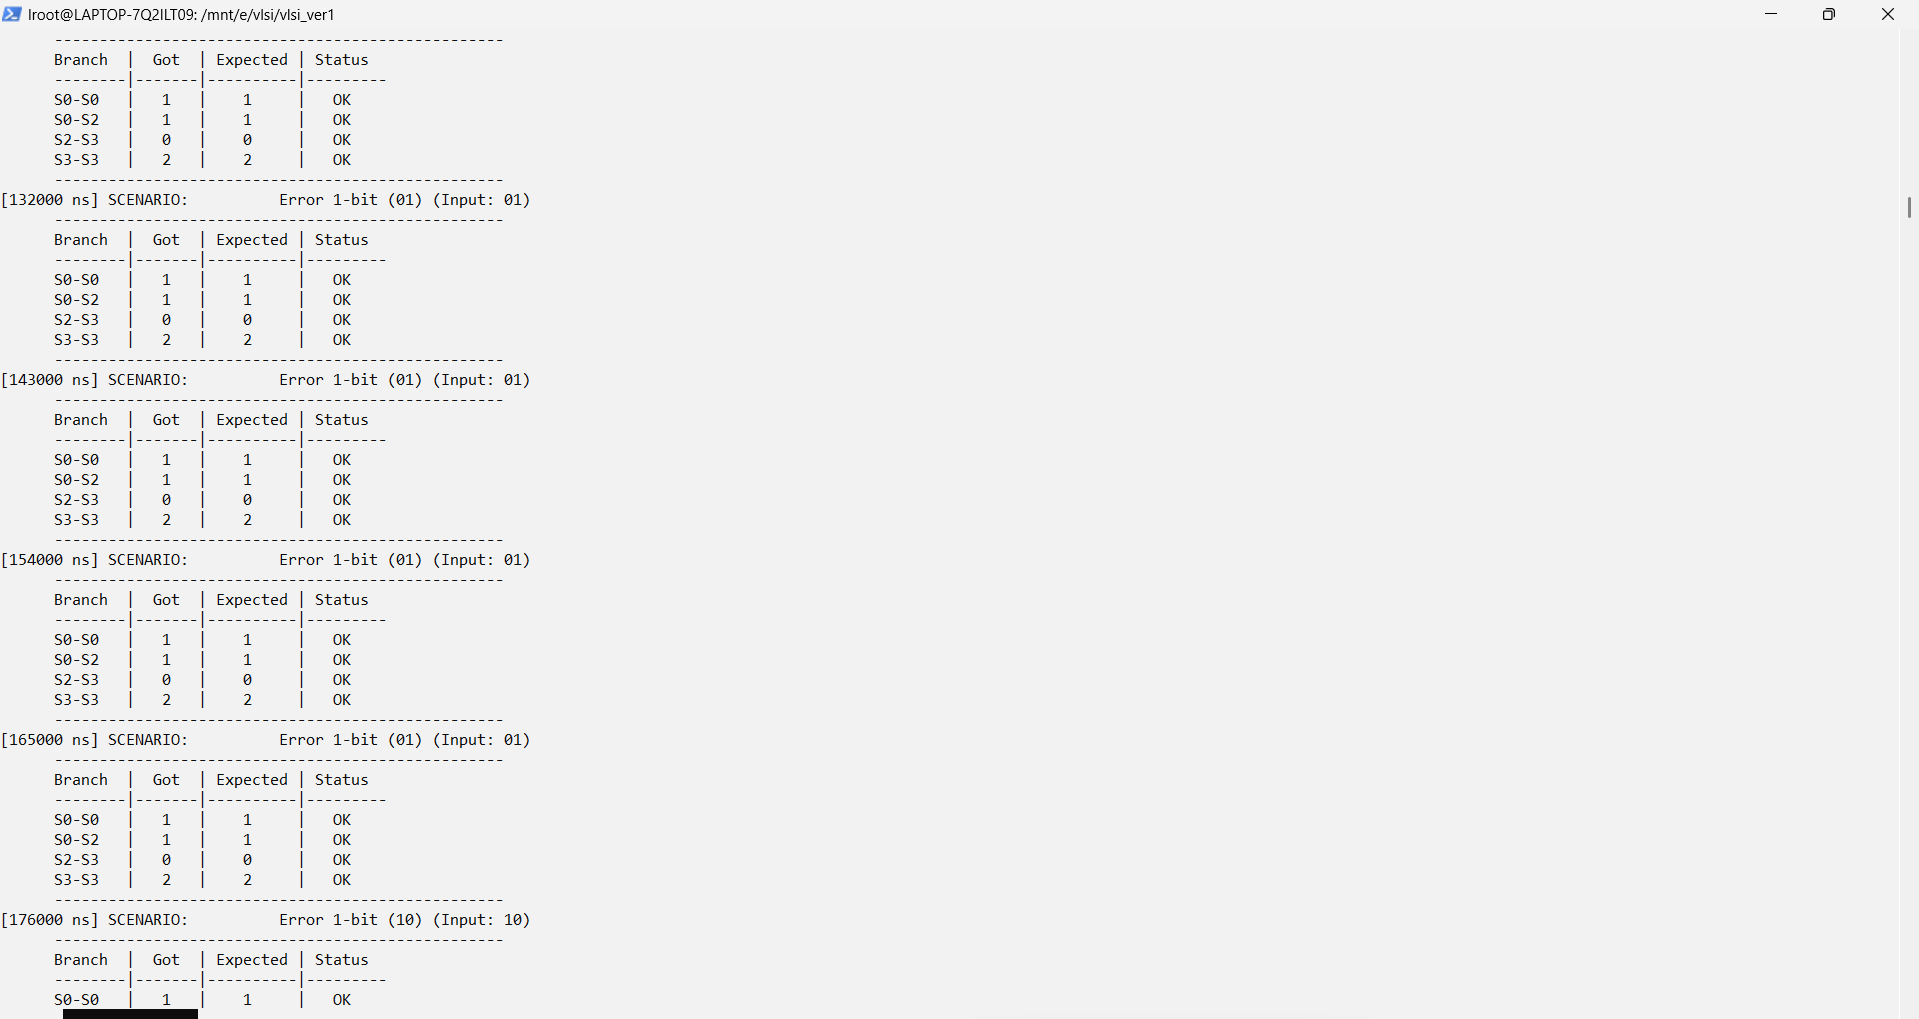
\includegraphics[width=1.0\textwidth]{bmu_log_part1.png}
    \caption{Log mô phỏng BMU - Phần 1}
\end{figure}
\begin{figure}[H]
    \centering
    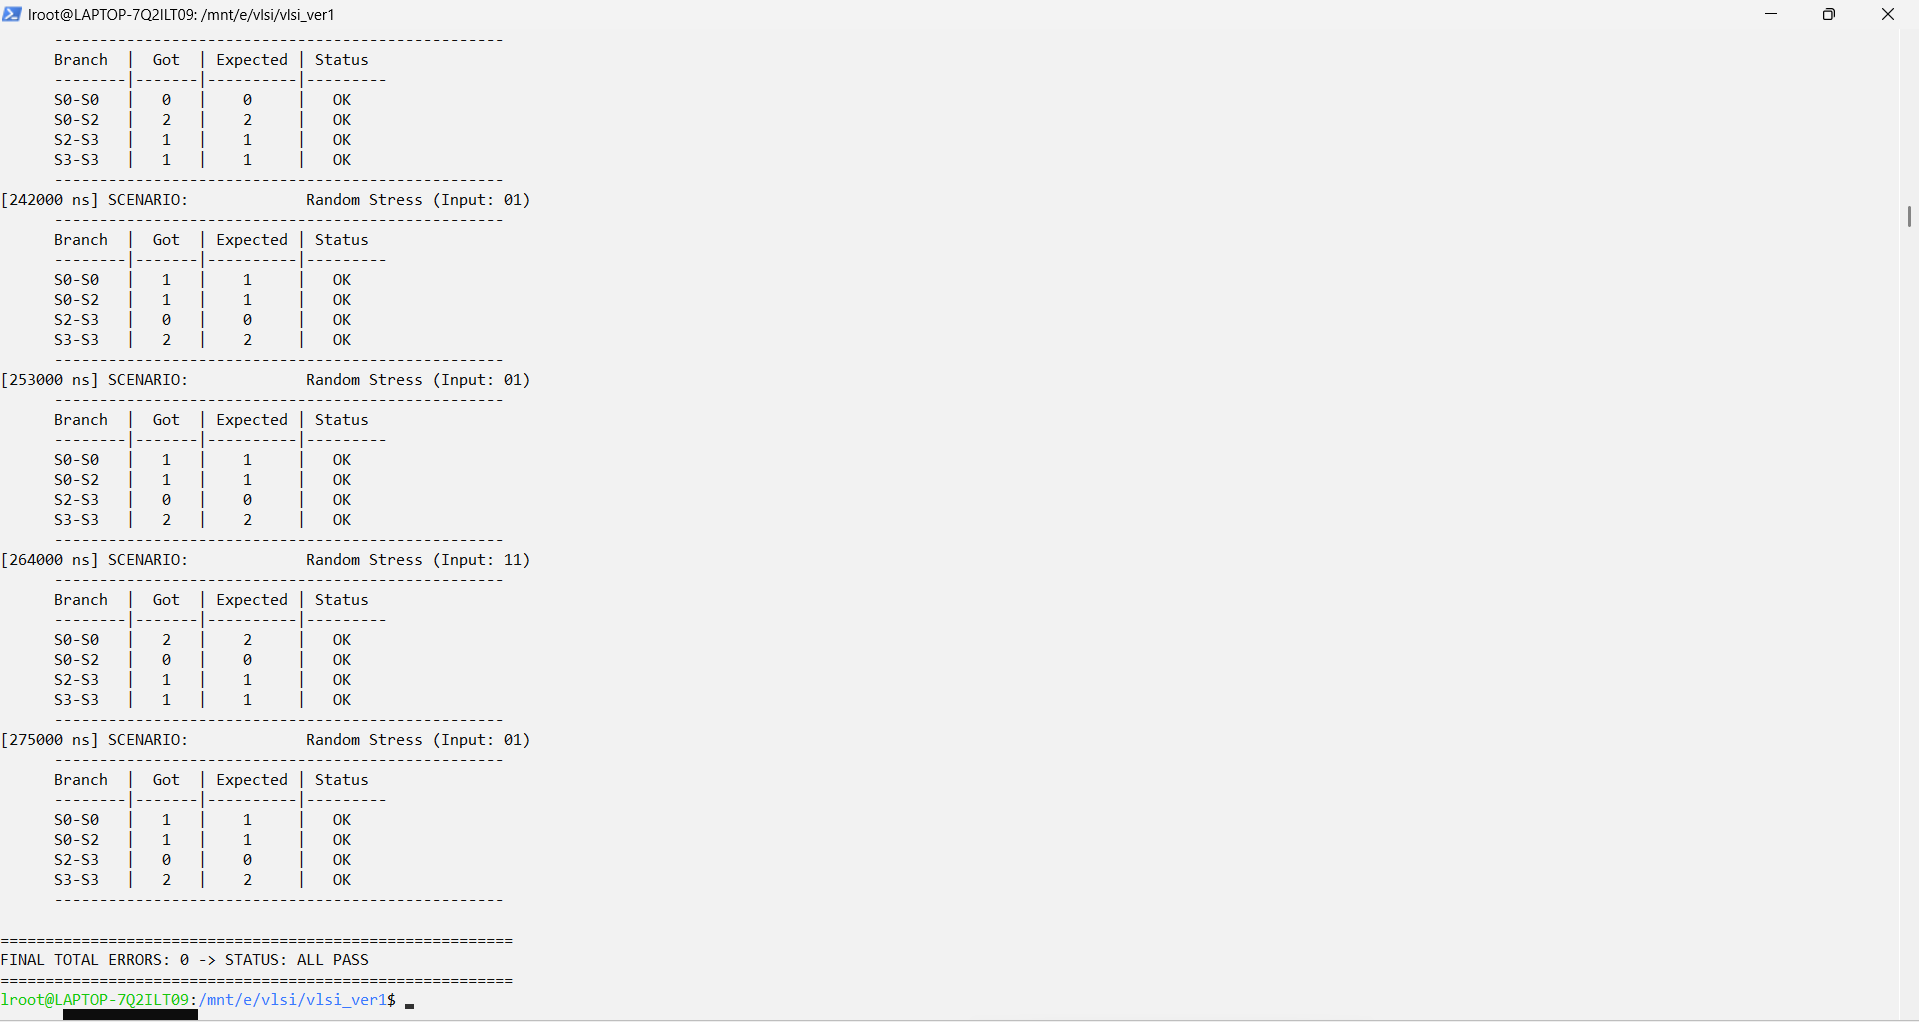
\includegraphics[width=1.0\textwidth]{bmu_log_part2.png}
    \caption{Log mô phỏng BMU - Phần 2}
\end{figure}
\begin{figure}[H]
    \centering
    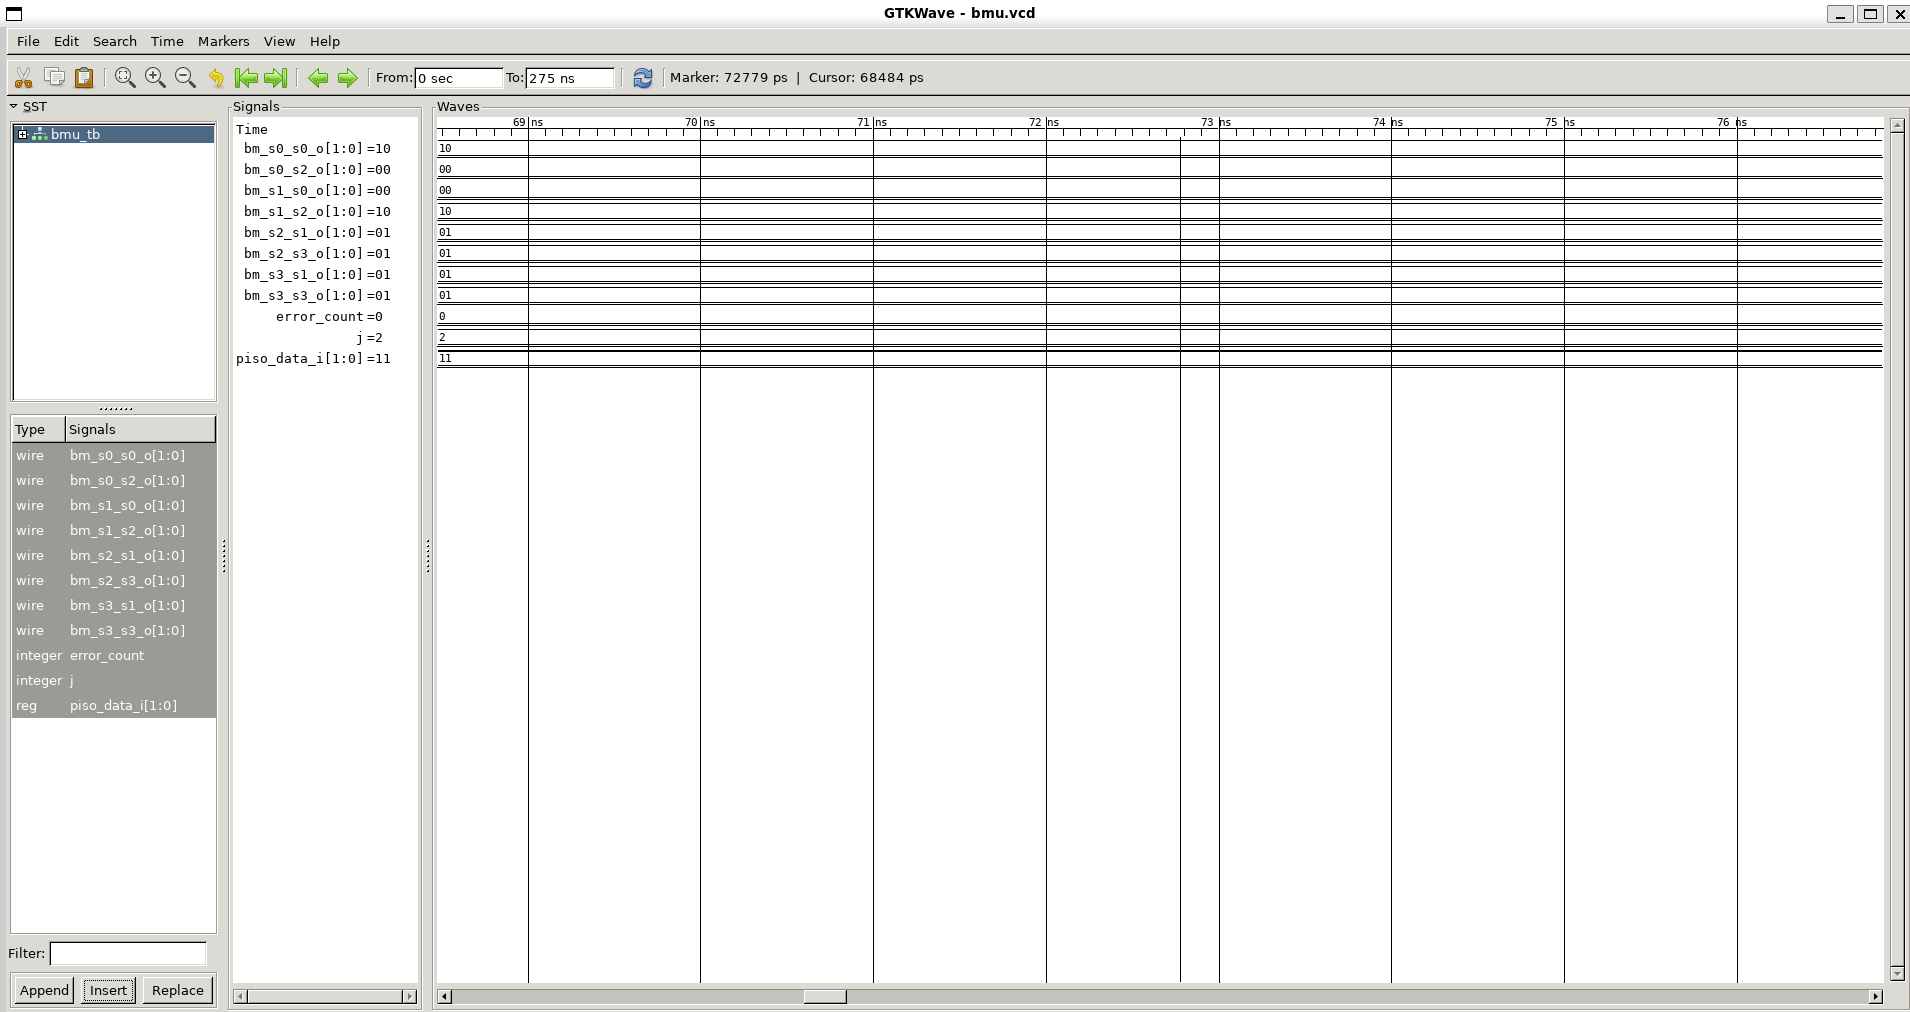
\includegraphics[width=1.0\textwidth]{bmu_wave.png}
    \caption{Giản đồ sóng tín hiệu BMU}
\end{figure}

% --- ACSU ---
\subsection{Khối Cộng - So sánh - Chọn (ACSU)}
Bảng dưới đây mô tả các kịch bản kiểm thử được thực hiện cho khối ACSU:

\begin{longtable}{|l|l|p{4cm}|p{4cm}|l|}
\hline
\textbf{ID} & \textbf{Tên Kịch Bản} & \textbf{Dữ liệu vào} & \textbf{Kỳ vọng} & \textbf{Kết quả} \\
\hline
\endhead
TC\_01 & Min Path Case & PM tăng dần, BM=1 & Chọn nhánh PM+BM nhỏ nhất & PASS \\
\hline
TC\_02 & Switching Winner & Đảo PM0 và PM1 & DEC bit thay đổi tương ứng & PASS \\
\hline
TC\_03 & Boundary Case & PM = 250 & Phép cộng không tràn, so sánh đúng & PASS \\
\hline
TC\_04 & Zero Case & PM=0, BM=0 & PM out=0, DEC chọn nhánh 0 & PASS \\
\hline
TC\_05 & Random Stress & Ngẫu nhiên & PM out = min(PMa+BMa, PMb+BMb) & PASS \\
\hline
\caption{Các kịch bản kiểm thử khối ACSU}
\end{longtable}

\begin{figure}[H]
    \centering
    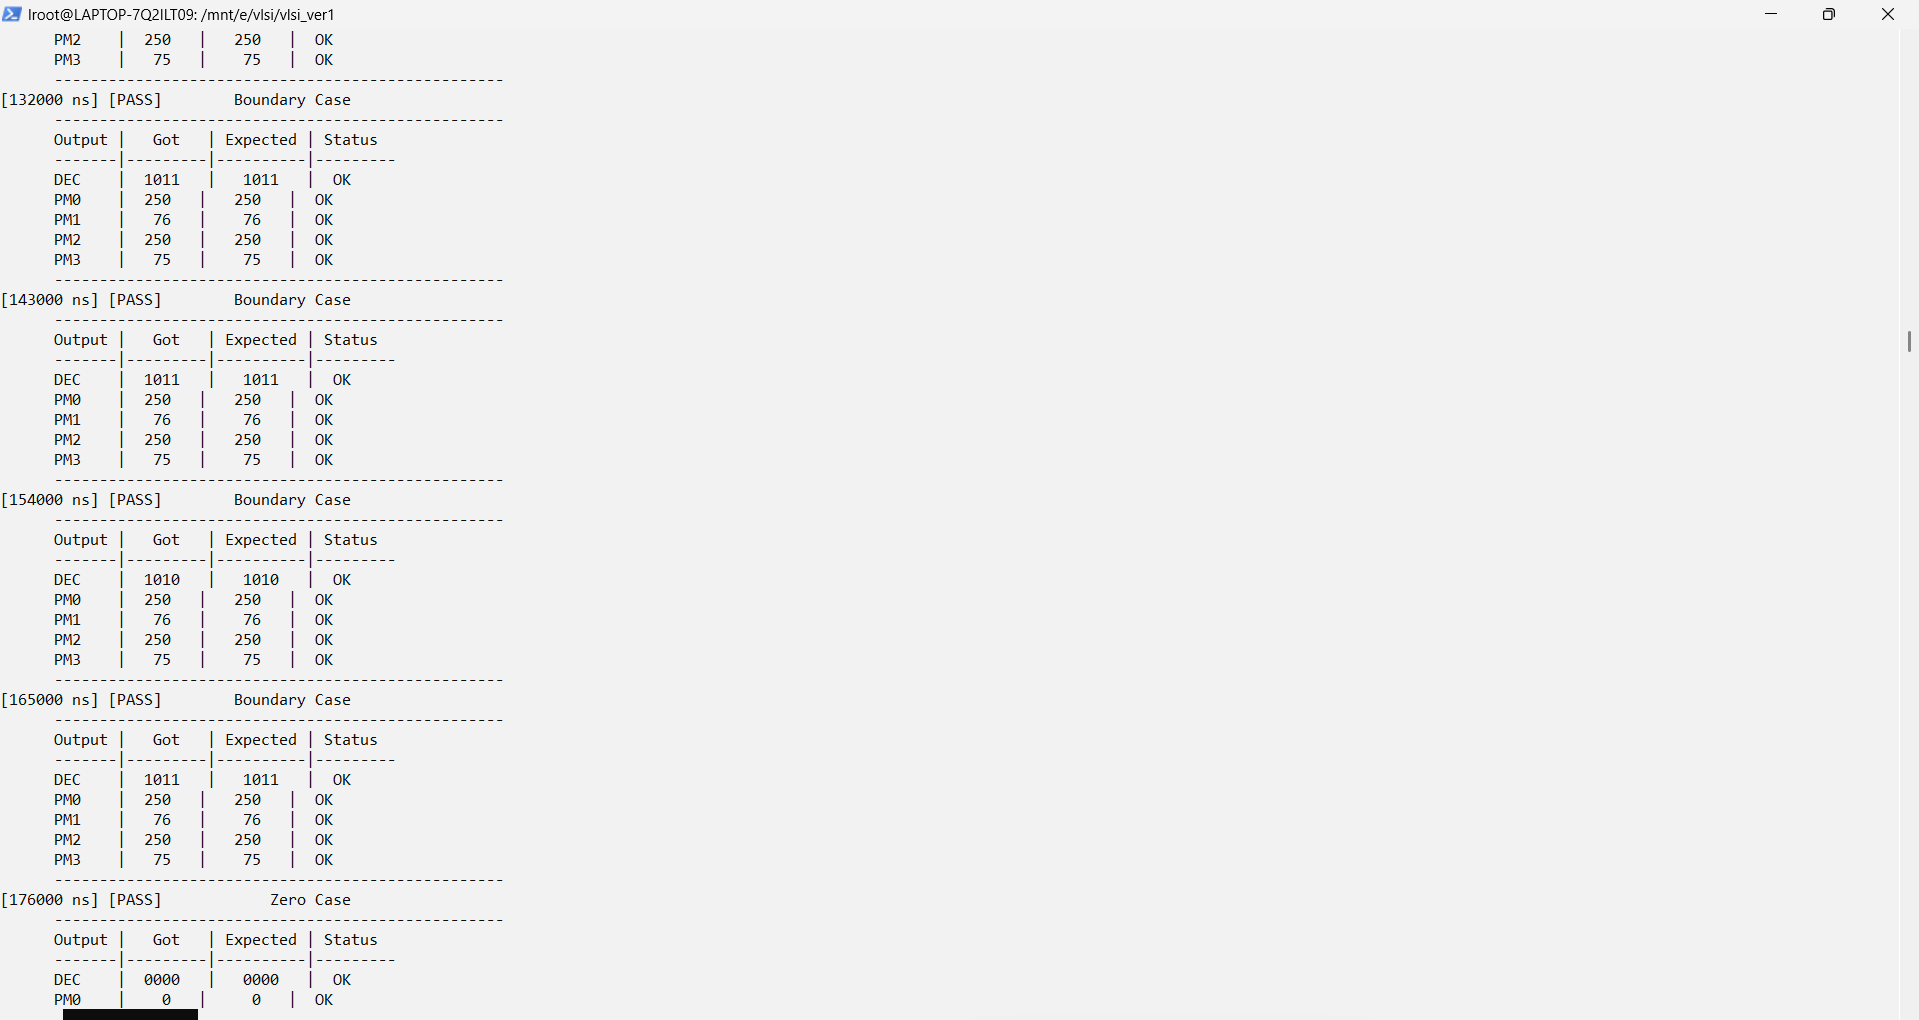
\includegraphics[width=1.0\textwidth]{acsu_log_part1.png}
    \caption{Log mô phỏng ACSU - Phần 1}
\end{figure}
\begin{figure}[H]
    \centering
    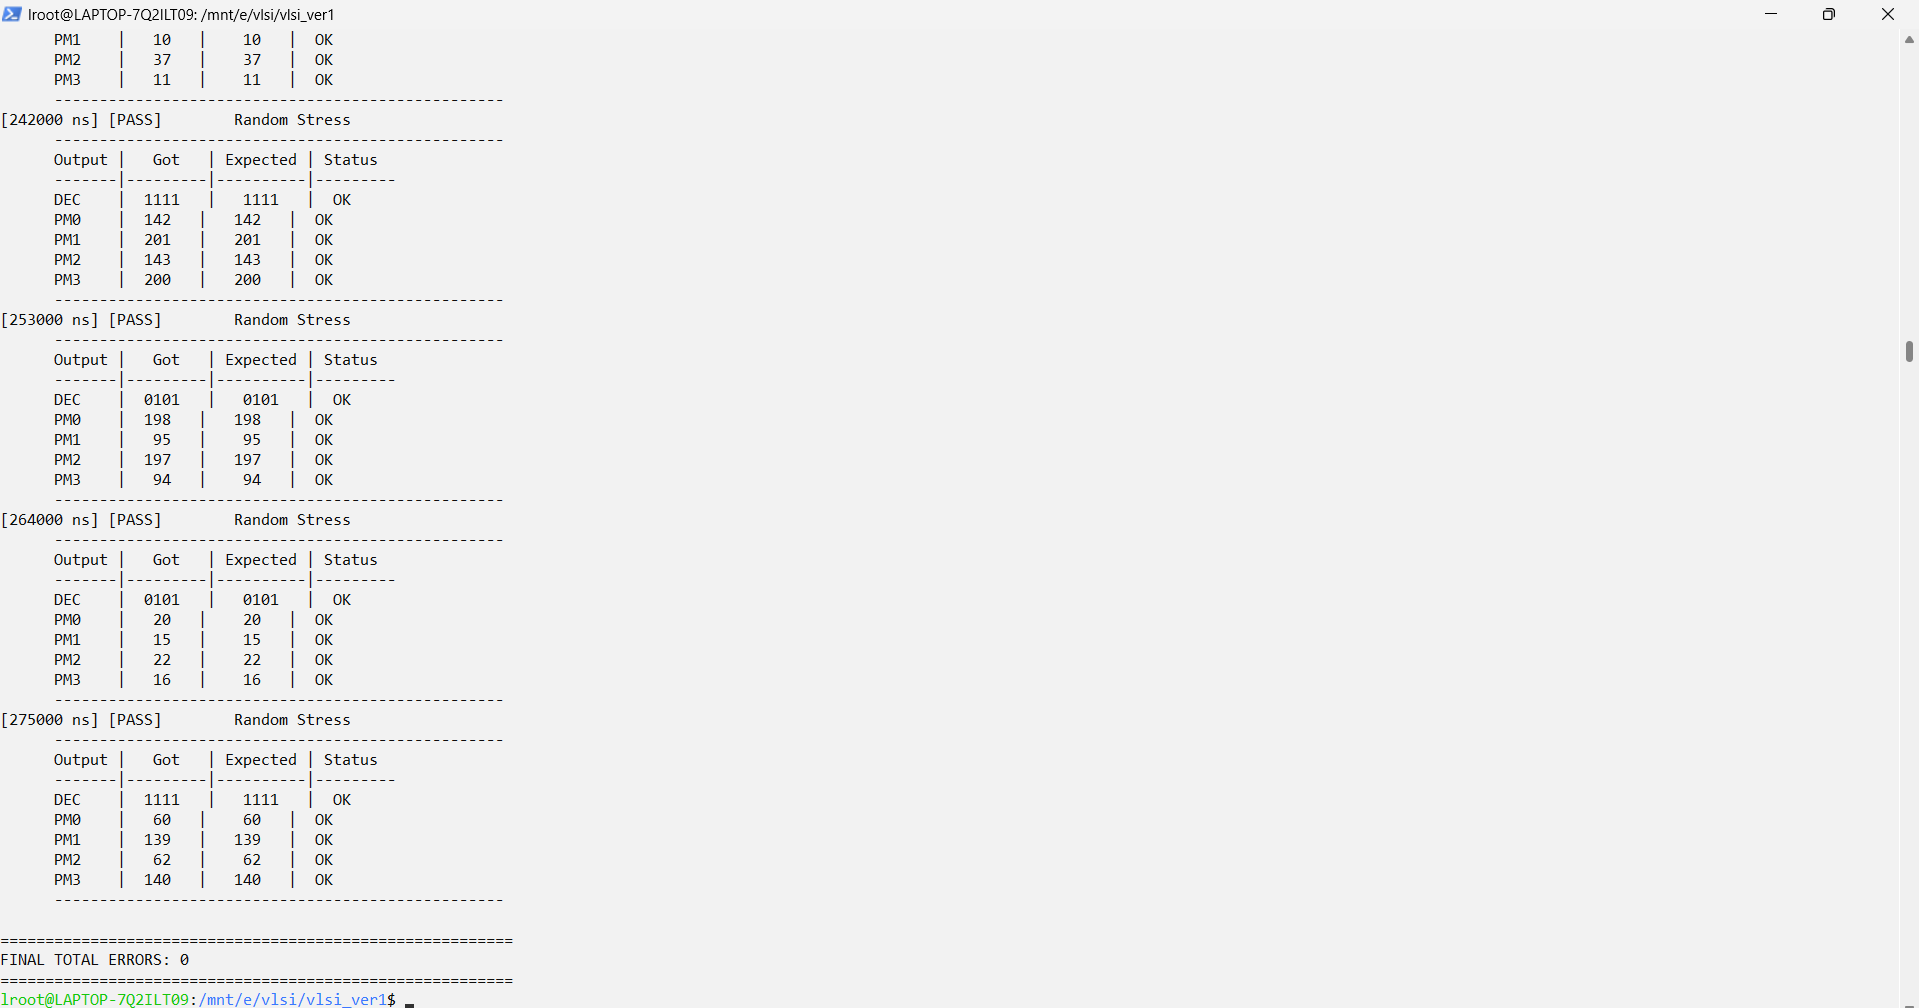
\includegraphics[width=1.0\textwidth]{acsu_log_part2.png}
    \caption{Log mô phỏng ACSU - Phần 2}
\end{figure}
\begin{figure}[H]
    \centering
    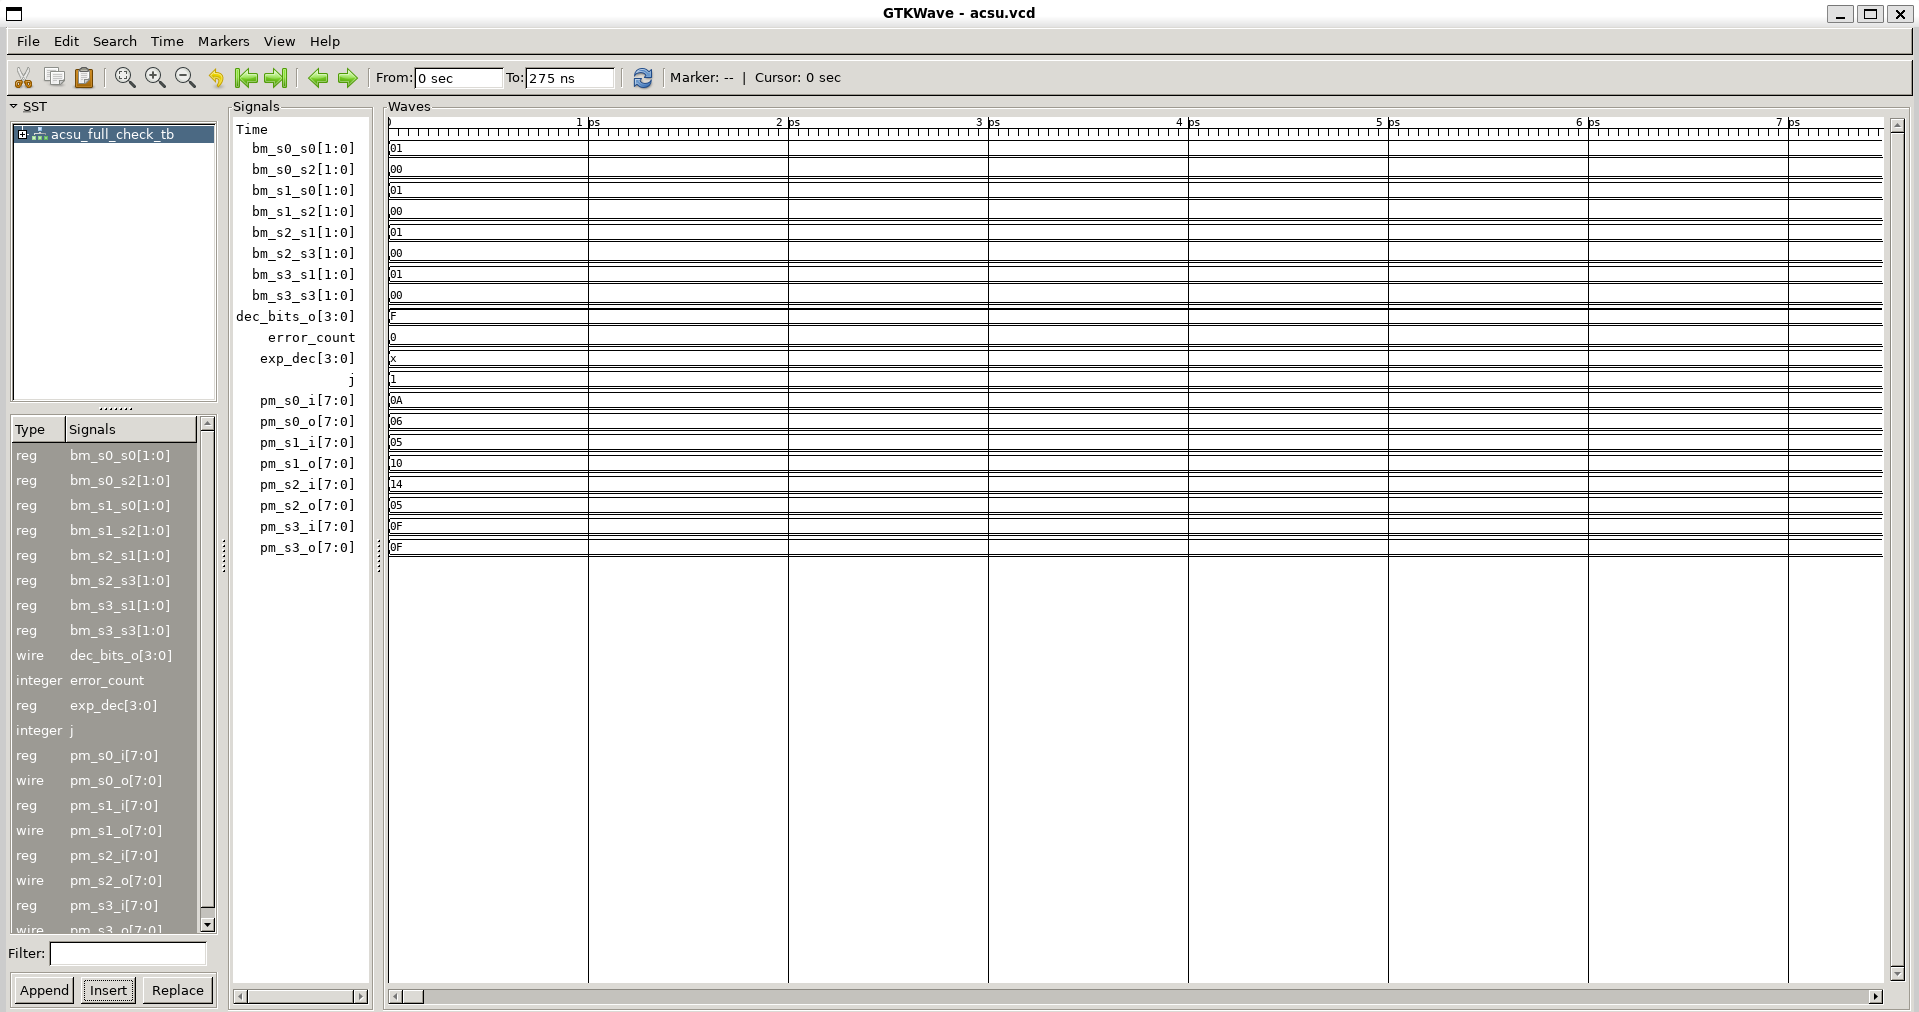
\includegraphics[width=1.0\textwidth]{acsu_wave.png}
    \caption{Giản đồ sóng tín hiệu ACSU}
\end{figure}

% --- PMU ---
\subsection{Khối quản lý Metric (PMU)}
Bảng dưới đây mô tả các kịch bản kiểm thử được thực hiện cho khối PMU:

\begin{longtable}{|l|l|p{3.5cm}|p{4cm}|l|}
\hline
\textbf{ID} & \textbf{Tên Kịch Bản} & \textbf{Hành động} & \textbf{Kỳ vọng} & \textbf{Kết quả} \\
\hline
\endhead
TC\_01 & Reset Check & Kéo rst\_n xuống 0 & S0=0, S1-S3=255 & PASS \\
\hline
TC\_02 & Update Enable & valid\_i=1, cấp dữ liệu mới & pm\_current\_o cập nhật đúng & PASS \\
\hline
TC\_03 & Keep Data & valid\_i=0, thay đổi input & Ngõ ra giữ nguyên & PASS \\
\hline
TC\_04 & Zero Stream & Tất cả input = 0 & Tất cả pm\_current\_o = 0 & PASS \\
\hline
TC\_05 & Random Stress & Ngẫu nhiên 5 chu kỳ & Ngõ ra cập nhật chính xác & PASS \\
\hline
\caption{Các kịch bản kiểm thử khối PMU}
\end{longtable}

\begin{figure}[H]
    \centering
    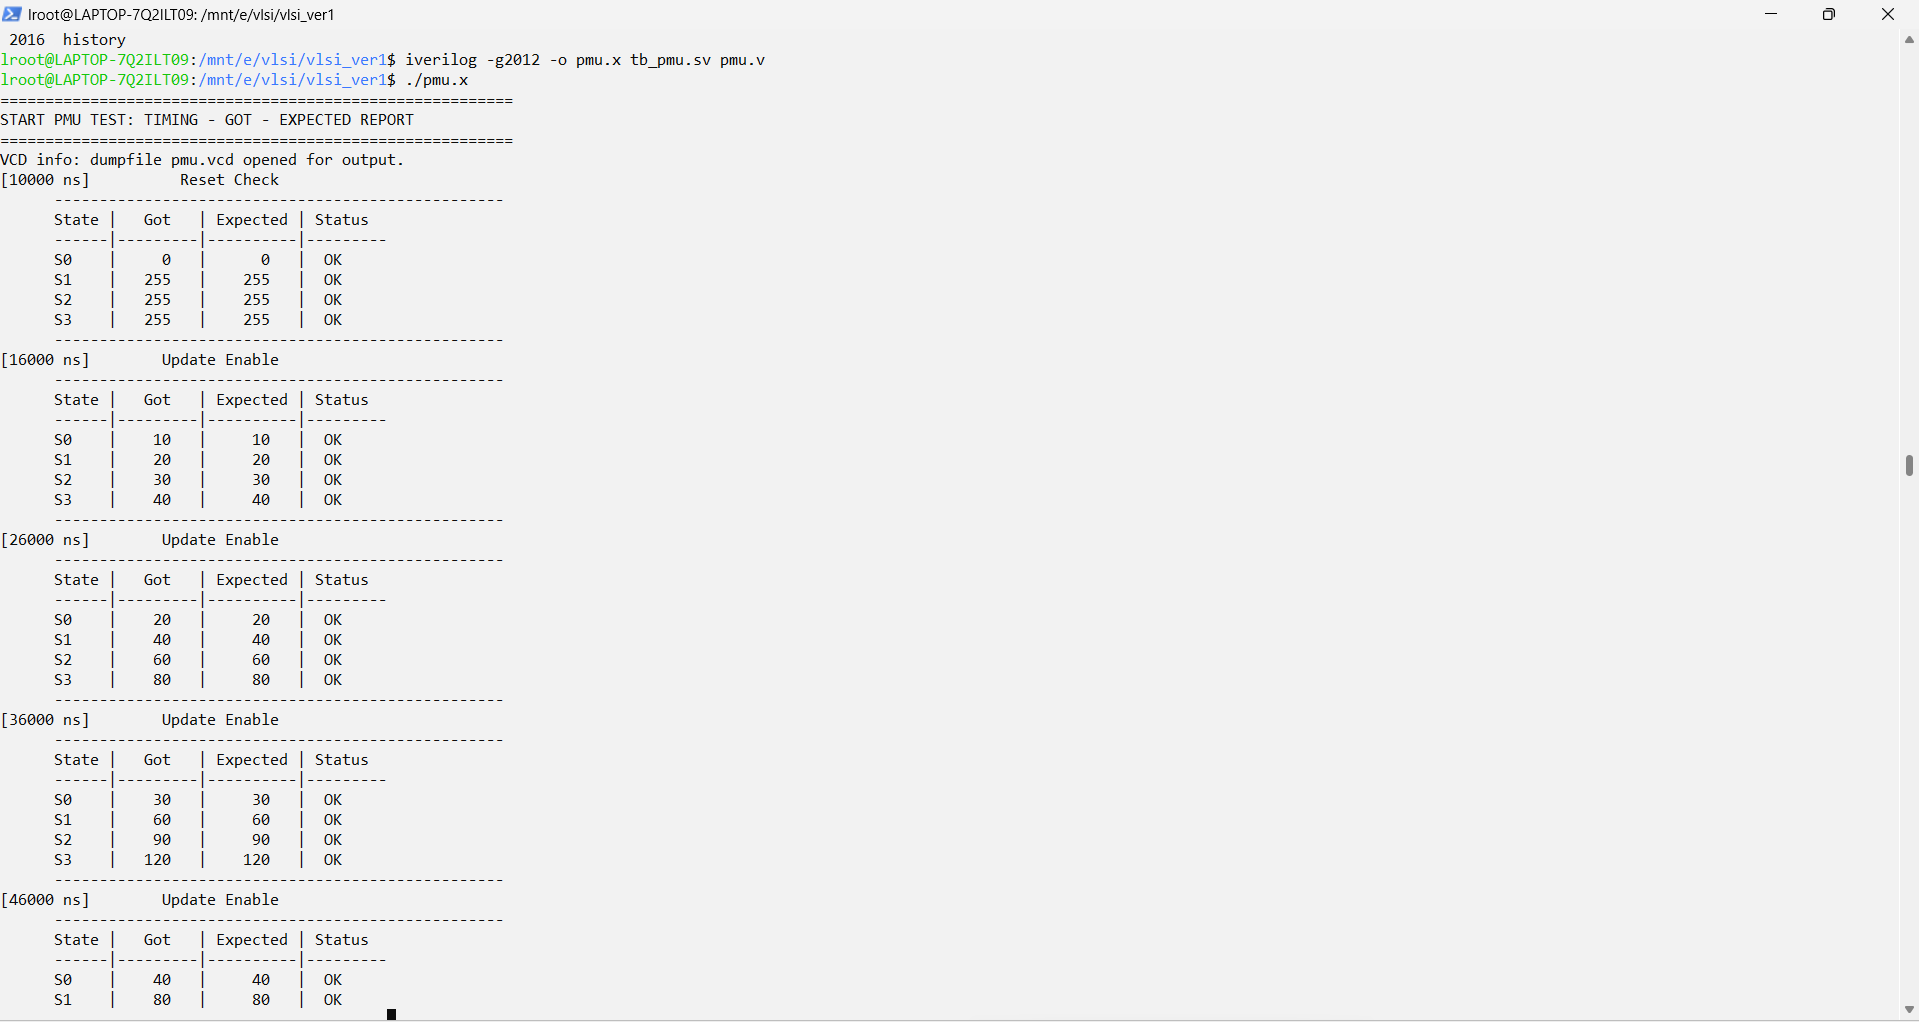
\includegraphics[width=1.0\textwidth]{pmu_log_part1.png}
    \caption{Log mô phỏng PMU - Phần 1}
\end{figure}
\begin{figure}[H]
    \centering
    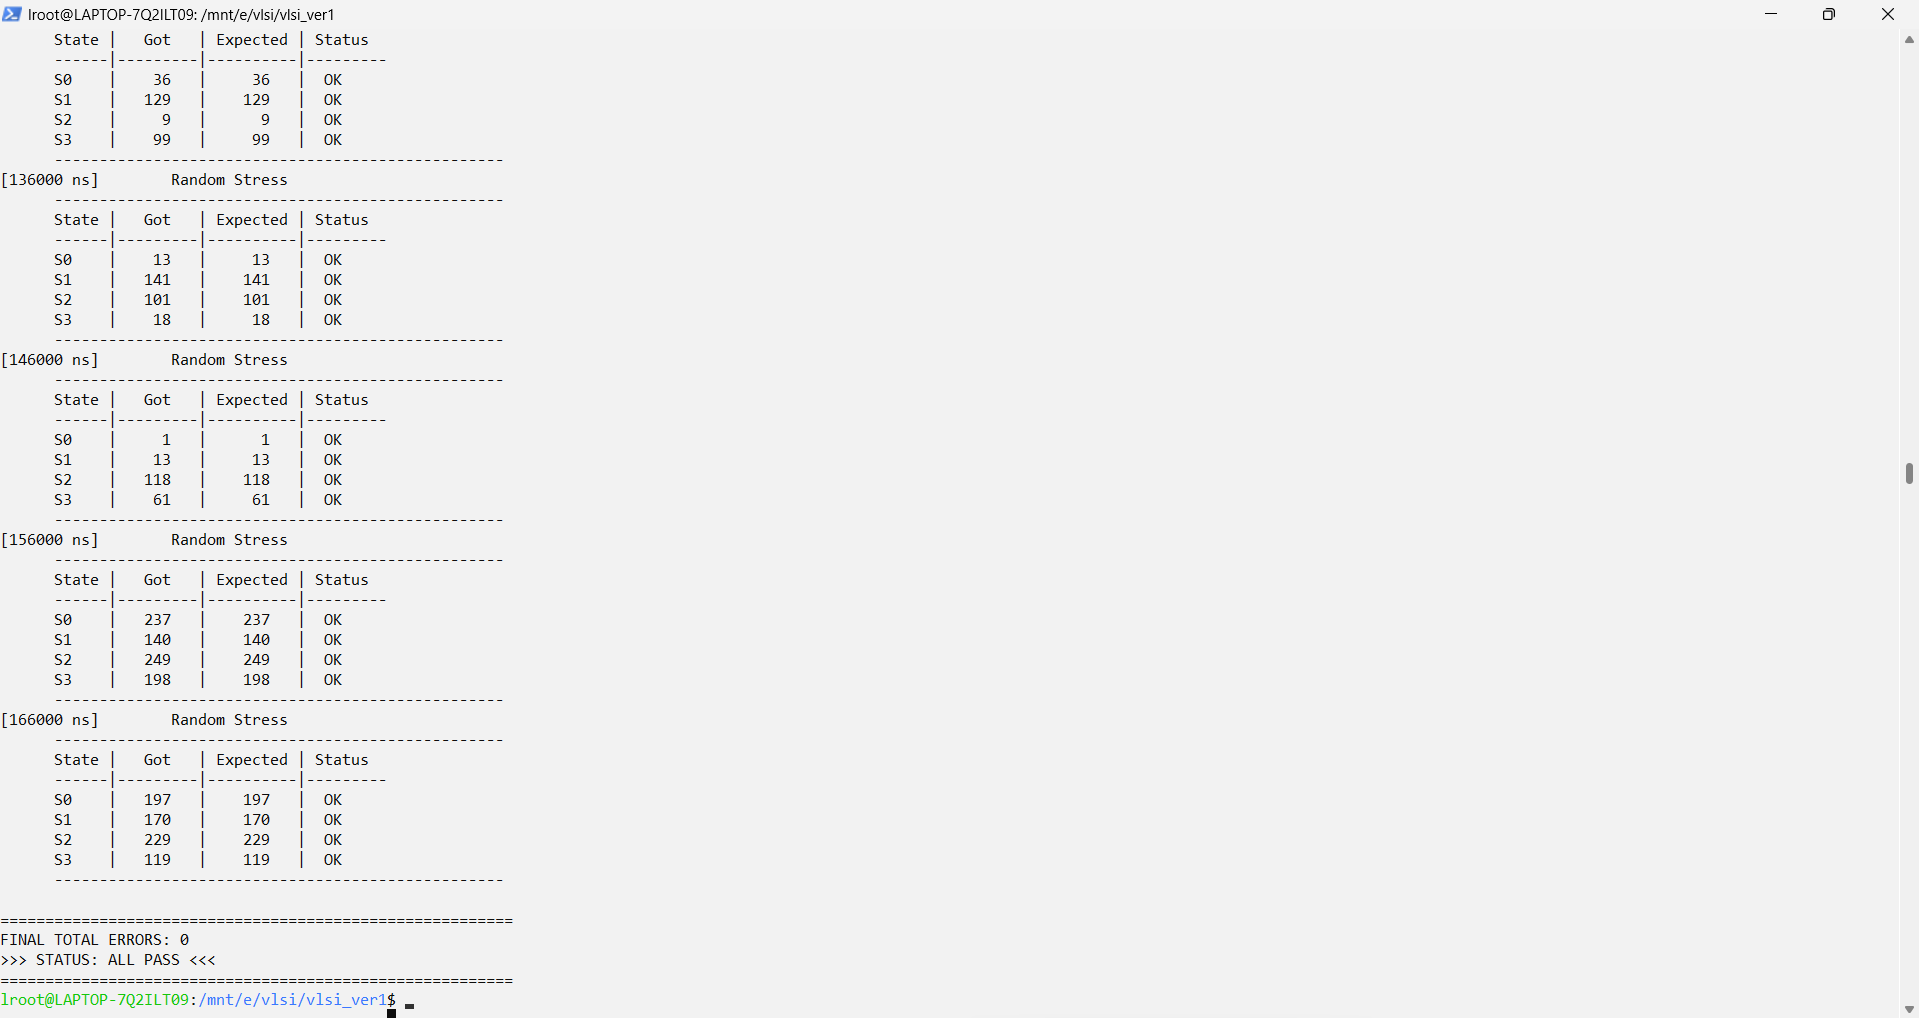
\includegraphics[width=1.0\textwidth]{pmu_log_part2.png}
    \caption{Log mô phỏng PMU - Phần 2}
\end{figure}
\begin{figure}[H]
    \centering
    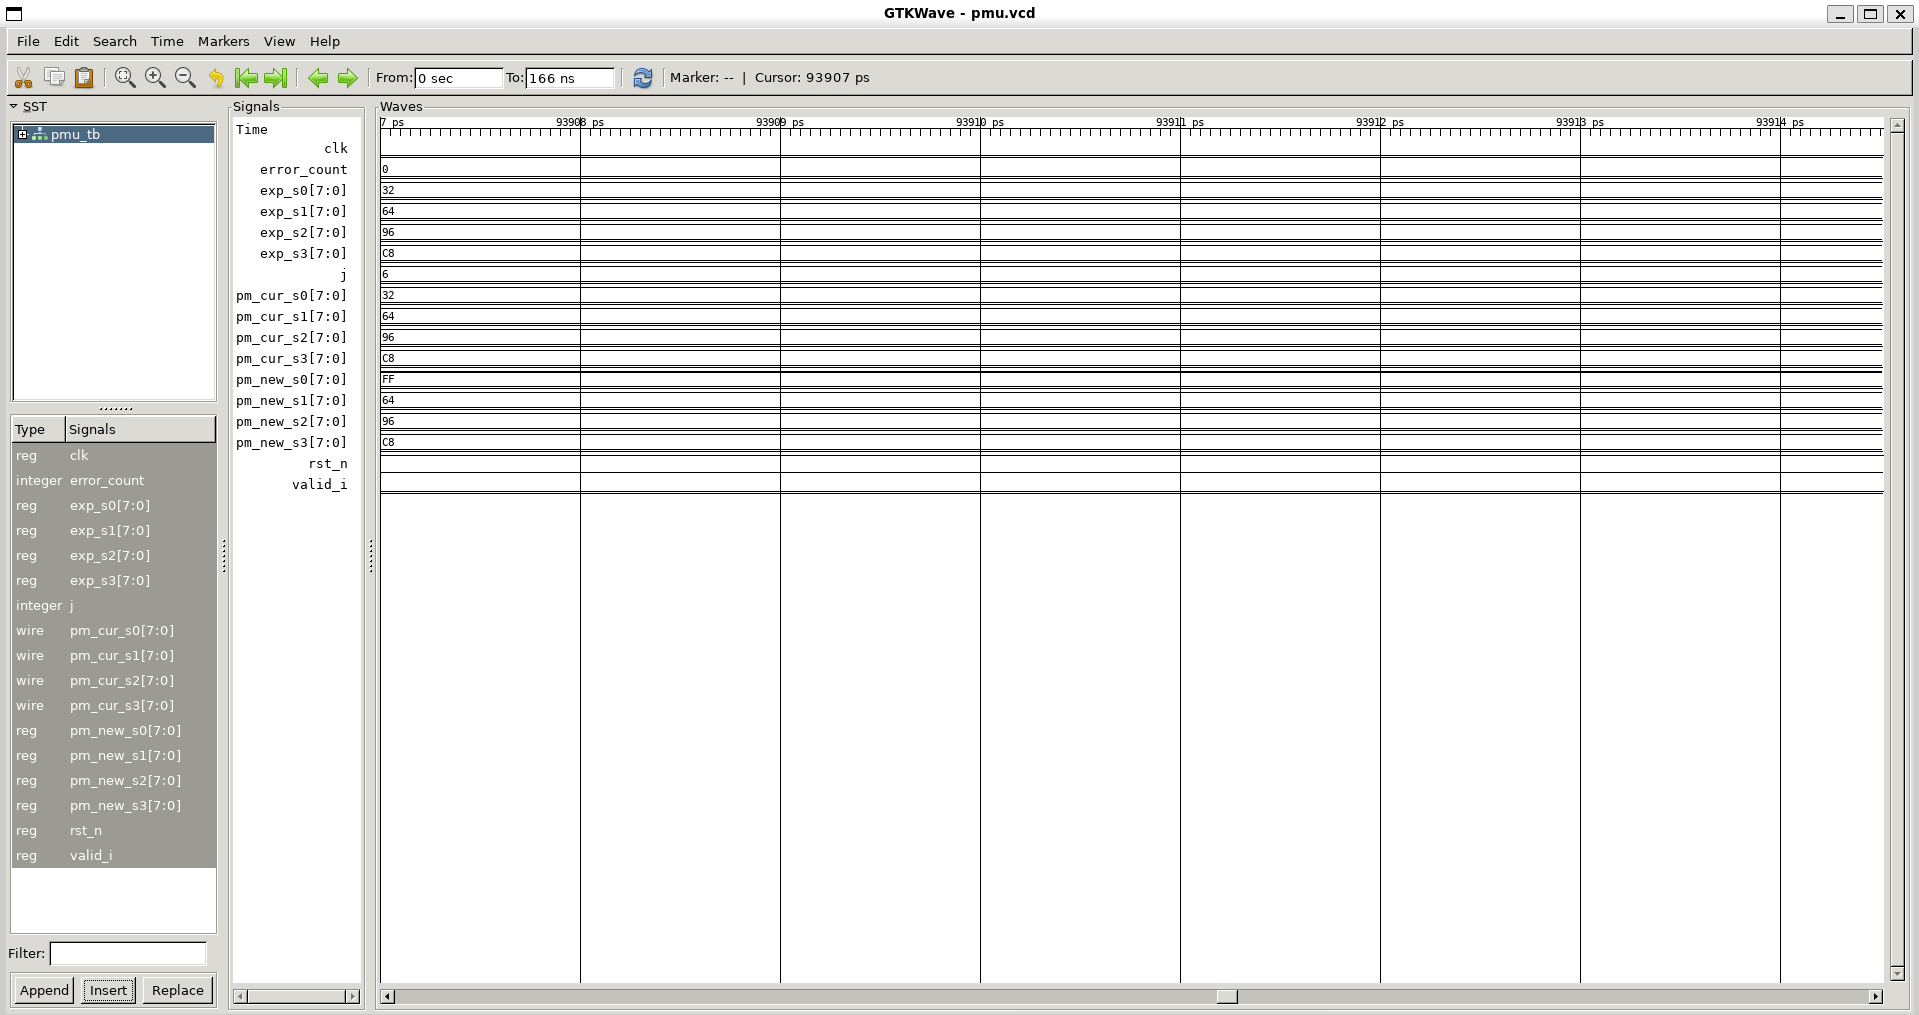
\includegraphics[width=1.0\textwidth]{pmu_wave.png}
    \caption{Giản đồ sóng tín hiệu PMU}
\end{figure}

% --- TBU ---
\subsection{Khối truy vết (TBU)}
Bảng dưới đây mô tả các kịch bản kiểm thử được thực hiện cho khối TBU:

\begin{longtable}{|l|l|p{3.5cm}|p{4cm}|l|}
\hline
\textbf{ID} & \textbf{Tên Kịch Bản} & \textbf{Hành động} & \textbf{Kỳ vọng} & \textbf{Kết quả} \\
\hline
\endhead
TC\_01 & Reset Check & Kích hoạt rst\_n & valid\_o=0, decoded\_bit=0 & PASS \\
\hline
TC\_02 & Pipeline Filling & Nạp 14 chu kỳ & valid\_o giữ mức 0 & PASS \\
\hline
TC\_03 & Start Decoding & Chu kỳ thứ 15 & valid\_o chuyển lên 1 & PASS \\
\hline
TC\_04 & Data Traceback & Nạp chuỗi bit '1' qua S2 & decoded\_bit\_o = 1 & PASS \\
\hline
TC\_05 & Valid\_i Gating & Tắt valid\_i & valid\_o về 0 ngay & PASS \\
\hline
TC\_06 & Winner Switching & PM\_S3 nhỏ nhất & Chọn bit từ history\_s3 & PASS \\
\hline
\caption{Các kịch bản kiểm thử khối TBU}
\end{longtable}

\begin{figure}[H]
    \centering
    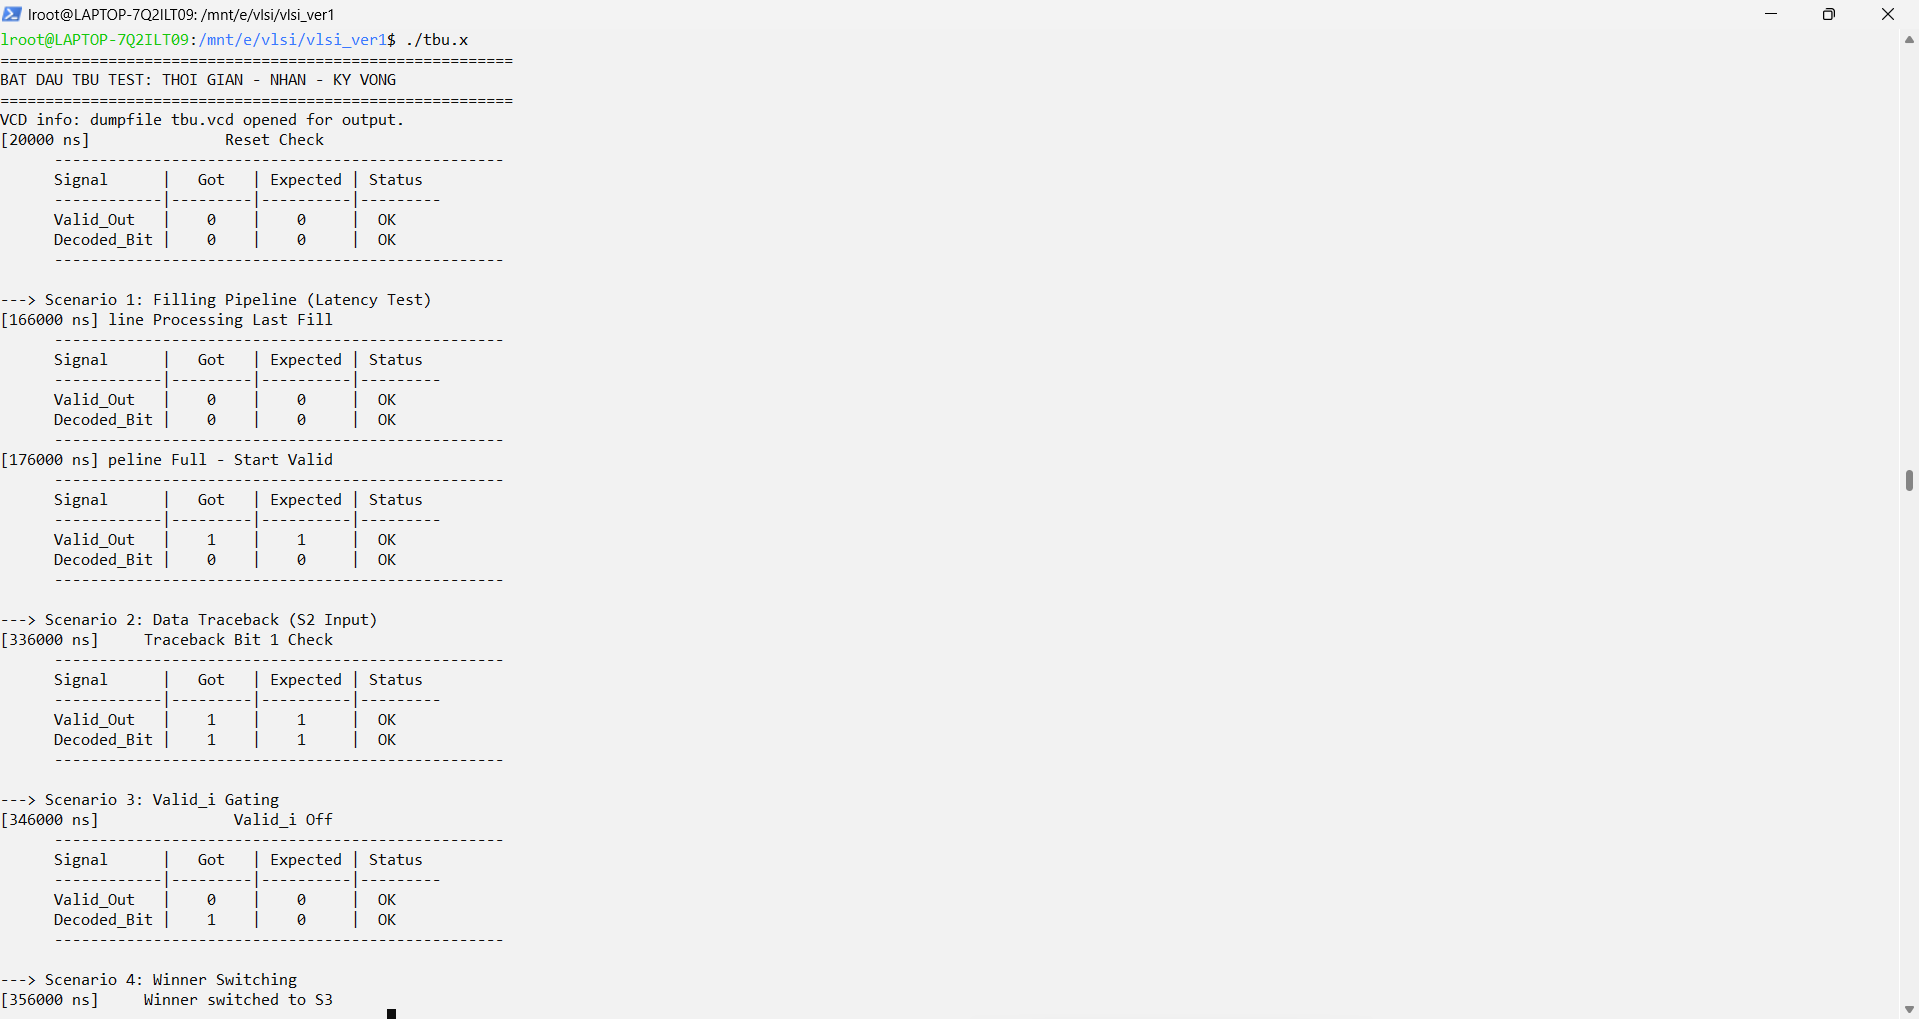
\includegraphics[width=1.0\textwidth]{tbu_log_part1.png}
    \caption{Log mô phỏng TBU - Phần 1}
\end{figure}
\begin{figure}[H]
    \centering
    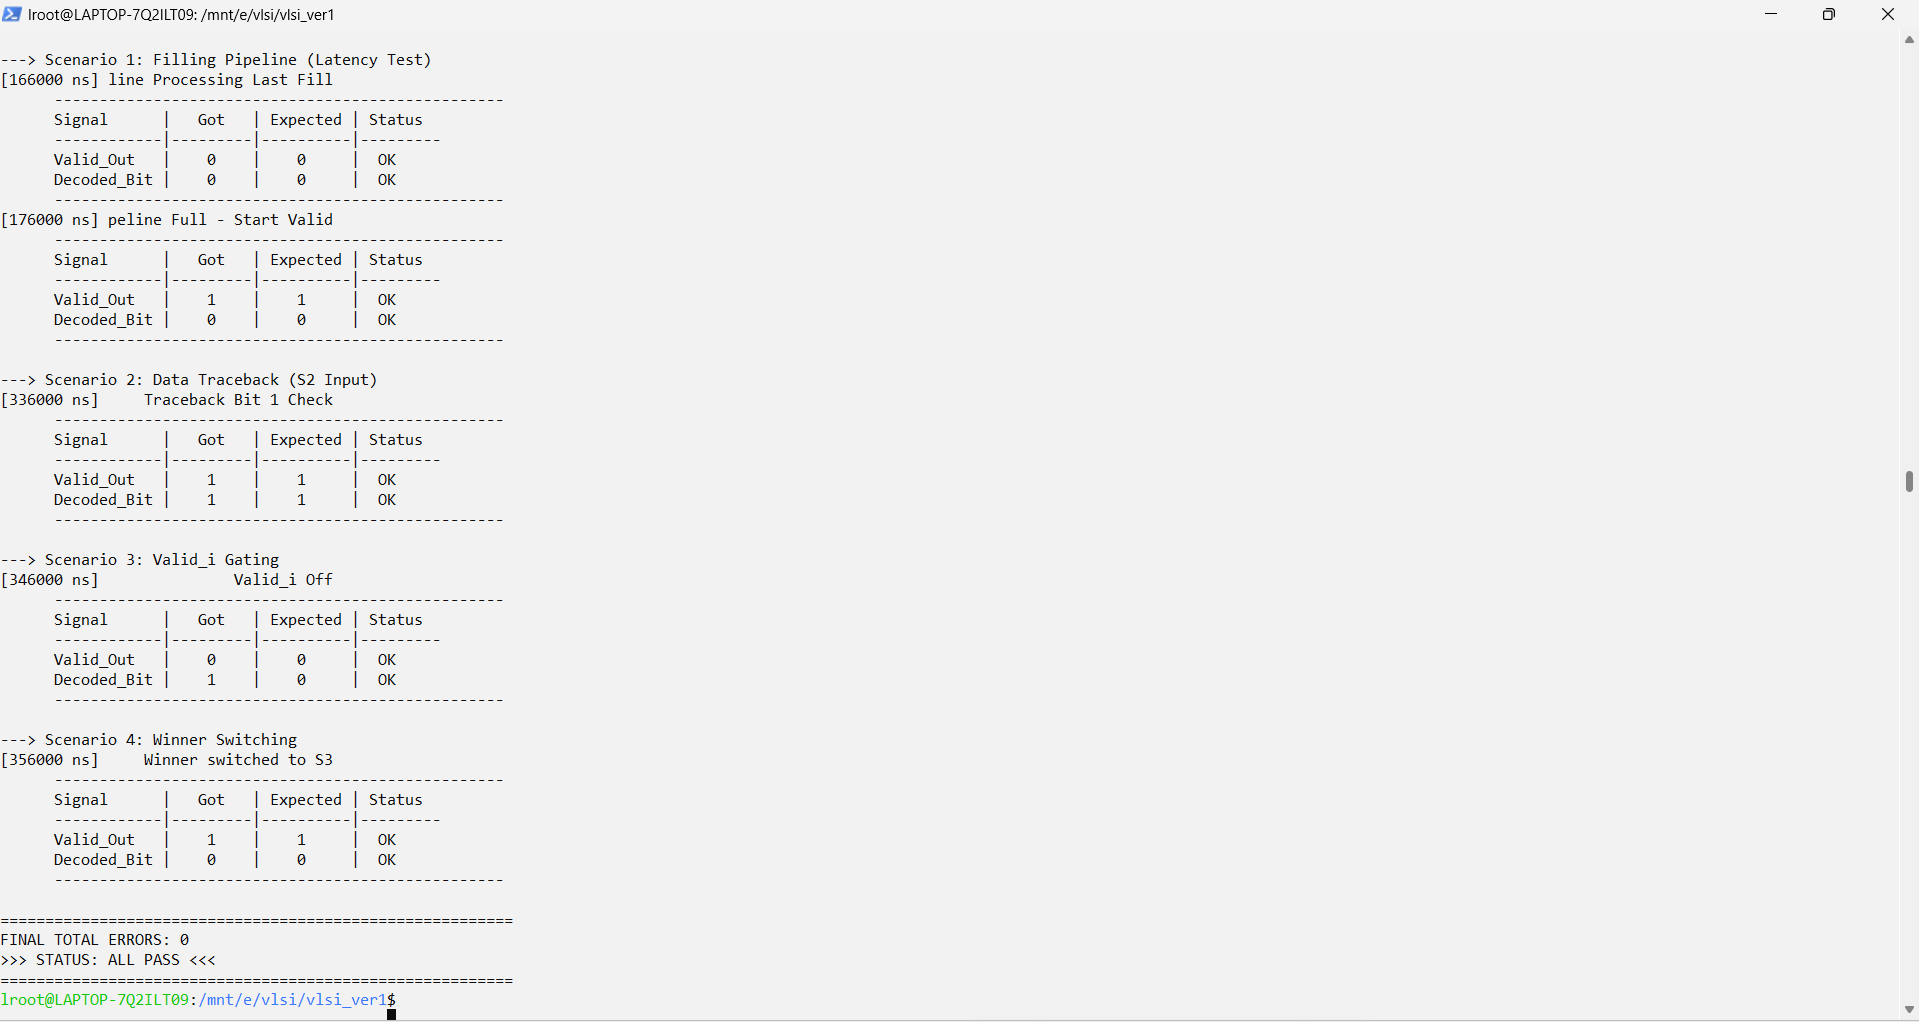
\includegraphics[width=1.0\textwidth]{tbu_log_part2.png}
    \caption{Log mô phỏng TBU - Phần 2}
\end{figure}
\begin{figure}[H]
    \centering
    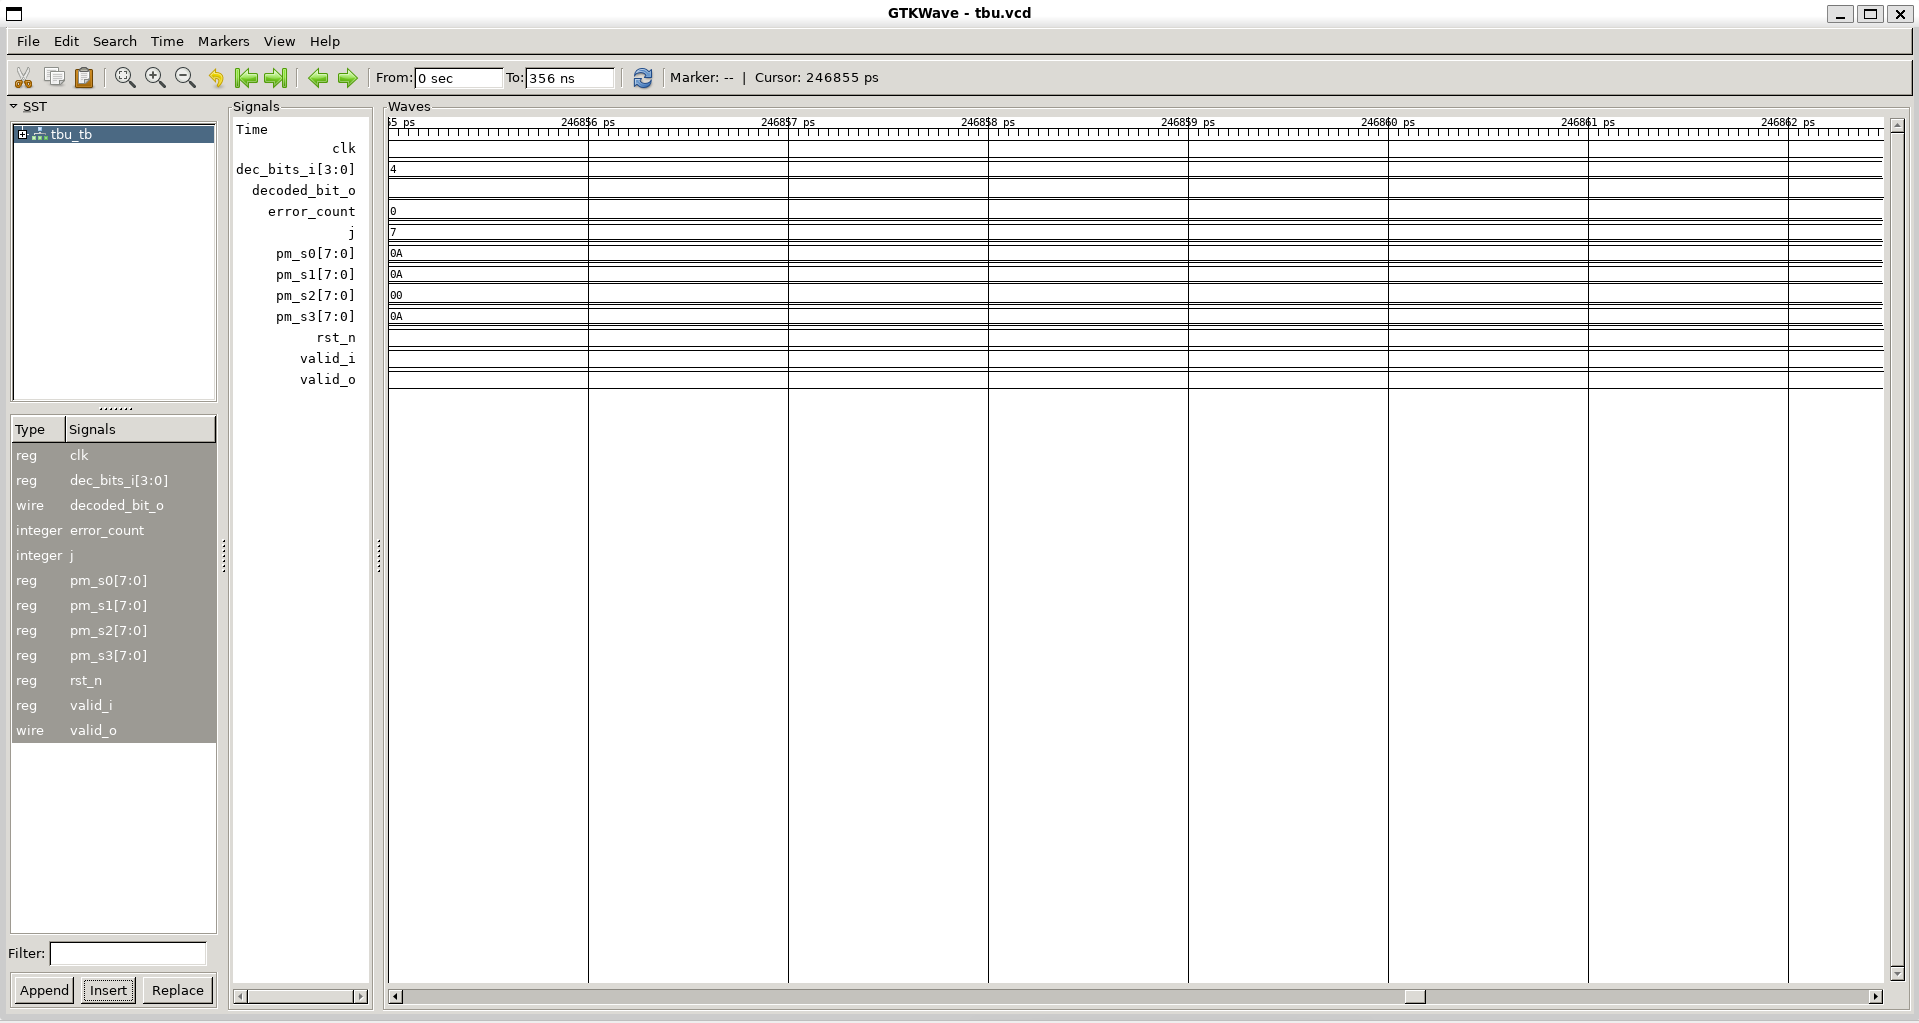
\includegraphics[width=1.0\textwidth]{tbu_wave.png}
    \caption{Giản đồ sóng tín hiệu TBU}
\end{figure}

% --- SIPO ---
\subsection{Khối chuyển đổi nối tiếp sang song song (SIPO)}
Bảng dưới đây mô tả các kịch bản kiểm thử được thực hiện cho khối SIPO:

\begin{longtable}{|l|l|l|p{4.5cm}|l|}
\hline
\textbf{ID} & \textbf{Tên Kịch Bản} & \textbf{Input} & \textbf{Kỳ vọng} & \textbf{Kết quả} \\
\hline
\endhead
TC\_01 & Reset Check & N/A & byte\_ready=0, data\_parallel=0 & PASS \\
\hline
TC\_02 & Normal Byte (0xA5) & 8'hA5 & data\_parallel=0xA5, byte\_ready=1 & PASS \\
\hline
TC\_03 & All Ones (0xFF) & 8'hFF & data\_parallel=0xFF, byte\_ready=1 & PASS \\
\hline
TC\_04 & All Zeros (0x00) & 8'h00 & data\_parallel=0x00, byte\_ready=1 & PASS \\
\hline
TC\_05 & Random Stress & Ngẫu nhiên & 5 byte khớp hoàn toàn & PASS \\
\hline
\caption{Các kịch bản kiểm thử khối SIPO}
\end{longtable}

\begin{figure}[H]
    \centering
    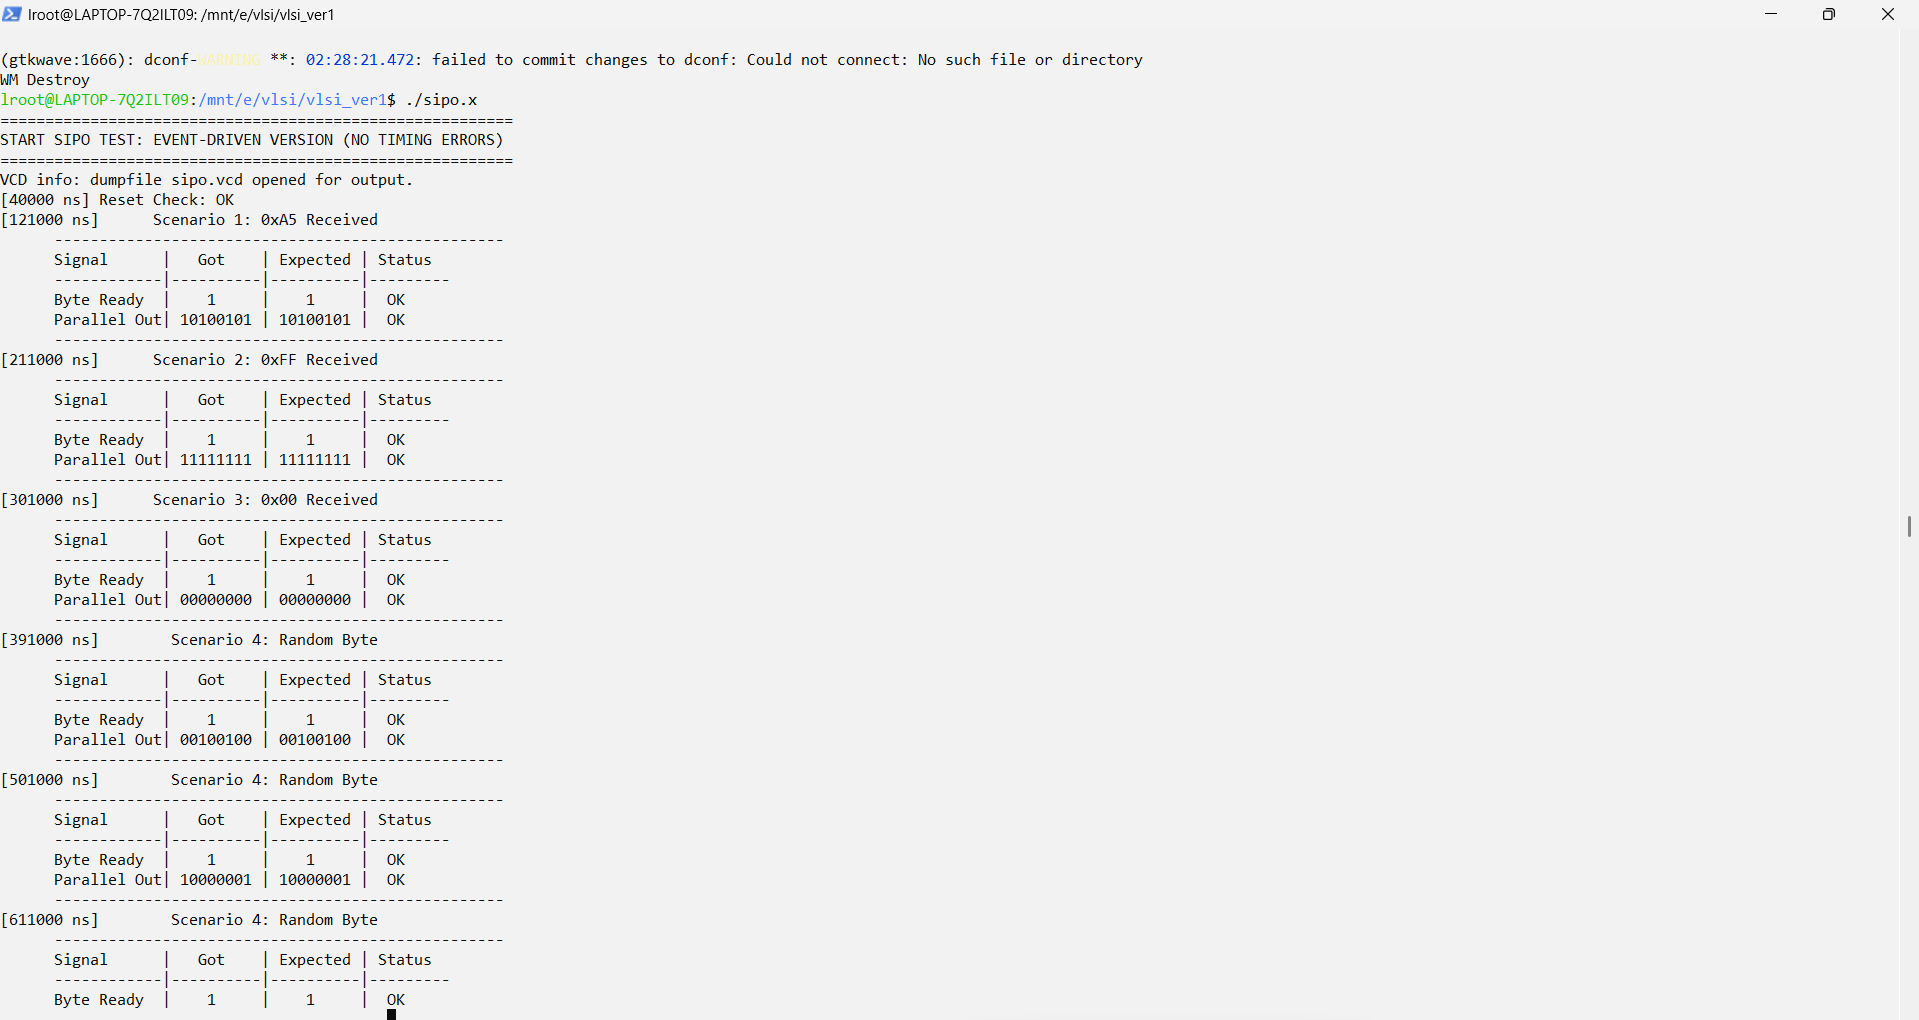
\includegraphics[width=1.0\textwidth]{sipo_log_part1.png}
    \caption{Log mô phỏng SIPO - Phần 1}
\end{figure}
\begin{figure}[H]
    \centering
    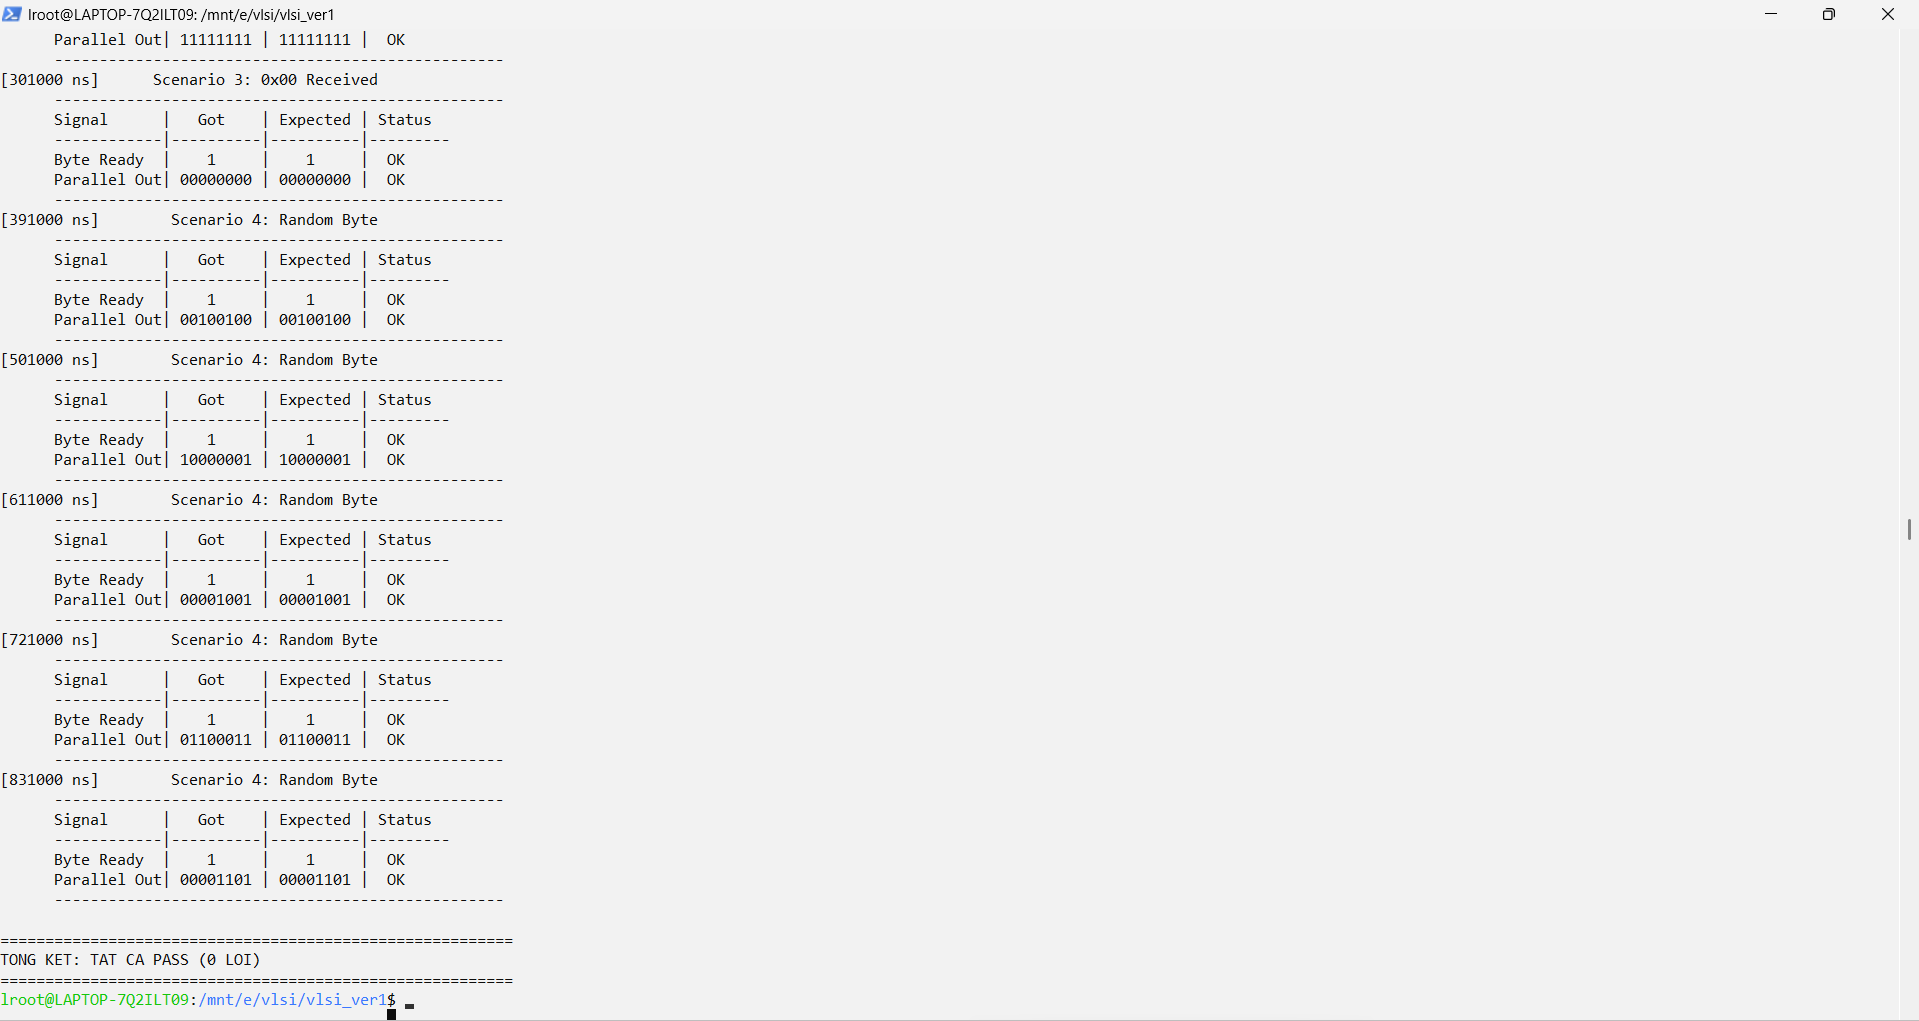
\includegraphics[width=1.0\textwidth]{sipo_log_part2.png}
    \caption{Log mô phỏng SIPO - Phần 2}
\end{figure}
\begin{figure}[H]
    \centering
    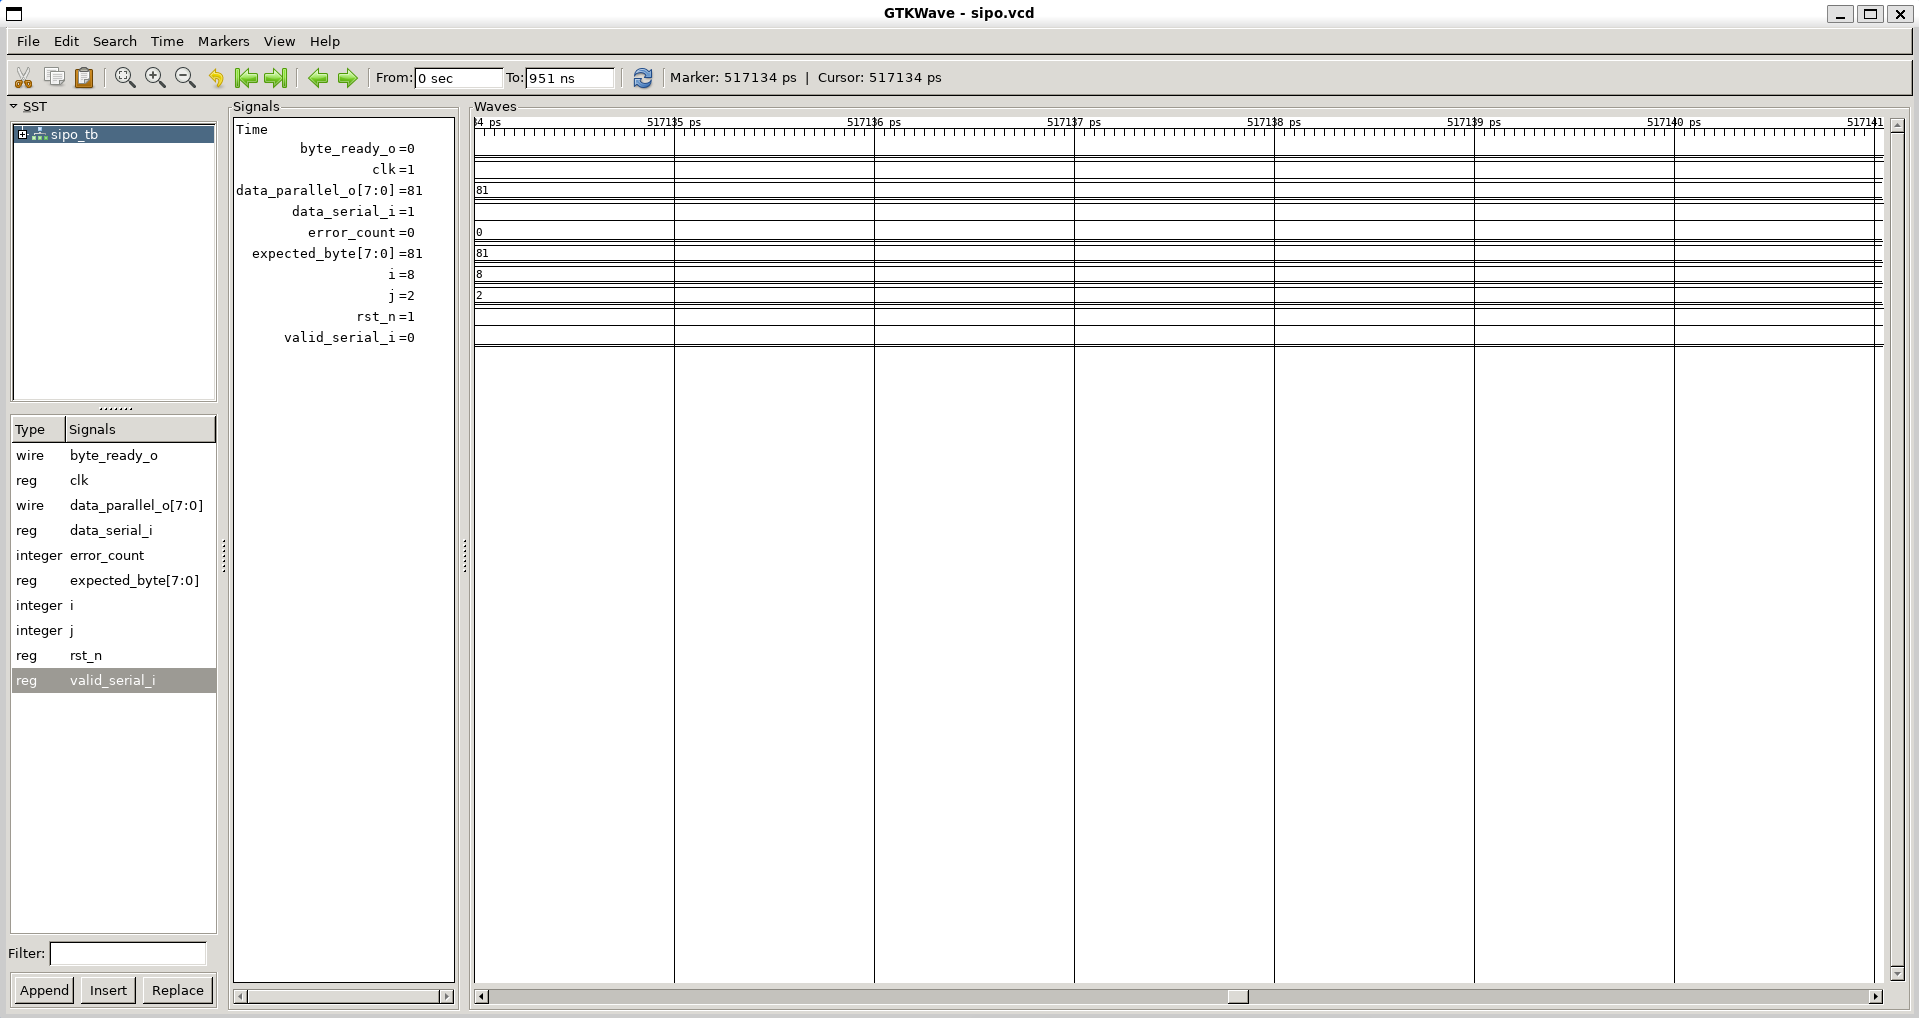
\includegraphics[width=1.0\textwidth]{sipo_wave.png}
    \caption{Giản đồ sóng tín hiệu SIPO}
\end{figure}
% ====================================================================
% SECTION 3.2.8: SYSTEM VERIFICATION
% ====================================================================
\subsection{Kiểm chứng toàn hệ thống (System Integration)}

Sau khi các khối đơn lẻ (Unit Level) đã hoạt động đúng, nhóm thực hiện tích hợp toàn bộ hệ thống và tiến hành kiểm thử mức hệ thống (System Level Verification). Mục tiêu là đảm bảo luồng dữ liệu từ Sync FIFO $\rightarrow$ PISO $\rightarrow$ Viterbi Core $\rightarrow$ SIPO hoạt động đồng bộ, đúng timing và quan trọng nhất là khả năng sửa lỗi của thuật toán.

\subsubsection{Kịch bản kiểm thử (Testcases)}

Hệ thống được kiểm tra với bộ Test Suite gồm 8 kịch bản chính, bao phủ từ hoạt động bình thường, khả năng sửa lỗi bit đến các trường hợp chịu tải cao (Stress test).

\begin{table}[H]
    \centering
    \caption{Tổng hợp kết quả các kịch bản kiểm thử hệ thống}
    \begin{tabularx}{\textwidth}{|l|l|X|l|}
    \hline
    \textbf{ID} & \textbf{Tên Testcase} & \textbf{Mô tả kịch bản} & \textbf{Kết quả} \\ \hline
    SYS\_01 & Sanity Check & Kiểm tra cơ bản: Gửi gói tin chuẩn, không lỗi. & \textbf{Pass} \\ \hline
    SYS\_02 & Full Range Sweep & Quét toàn bộ dải giá trị đầu vào (0x0000 - 0xFFFF). & \textbf{Pass} \\ \hline
    SYS\_03 & Single Bit Error & Gây nhiễu sai 1 bit ngẫu nhiên. Hệ thống phải tự sửa lại đúng. & \textbf{Pass} \\ \hline
    SYS\_04 & Multi-bit Error & Gây nhiễu sai 2-3 bit (Vượt quá khả năng sửa lỗi lý thuyết). & Mixed \\ \hline
    SYS\_05 & Burst Error & Kiểm tra khả năng chịu lỗi chùm (sai 4 bit liên tiếp). & Fail (Expected) \\ \hline
    SYS\_06 & Busy Ignore & Gửi dữ liệu khi cờ Busy=1 (Sync FIFO đầy). & \textbf{Pass} \\ \hline
    SYS\_07 & Continuous Stress & Gửi dữ liệu liên tục tốc độ cao (Back-to-back transaction). & \textbf{Pass} \\ \hline
    SYS\_08 & Reset Recovery & Reset hệ thống giữa chừng khi đang xử lý. & \textbf{Pass} \\ \hline
    \end{tabularx}
\end{table}

\subsubsection{Mã nguồn Testbench (Trích đoạn)}

Module kiểm thử tự động (\texttt{tb\_system\_top.sv}) được xây dựng với cơ chế "Self-checking". Dưới đây là trích đoạn Task gửi dữ liệu có hỗ trợ tiêm lỗi (Error Injection):

\begin{lstlisting}[language=Verilog, caption=Task gửi dữ liệu và tiêm lỗi trong Testbench]
// Task: Send 16-bit data packet
task send_packet(input [15:0] data, input [2:0] error_count);
    logic [15:0] corrupted_data;
    begin
        // Inject artificial error to test error correction capability
        corrupted_data = inject_error(data, error_count);
        
        // Handshake protocol with the system
        wait(!busy_o);      // Wait for system ready
        @(posedge clk);
        dvalid_i = 1'b1;    // Assert Valid
        data_i   = corrupted_data;
        @(posedge clk);
        dvalid_i = 1'b0;
    end
endtask
\end{lstlisting}

\subsubsection{Kết quả mô phỏng}

Hình \ref{fig:test_summary} dưới đây là báo cáo tổng hợp tự động từ Testbench. Hệ thống đạt tỷ lệ thành công tuyệt đối (100\%) với các trường hợp dữ liệu sạch (Clean) và lỗi 1 bit (Error 1b).

\begin{figure}[H]
    \centering
    % Rename file 2dfaac... to test_summary.jpg
    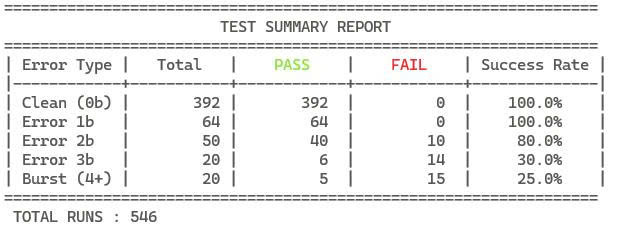
\includegraphics[width=0.8\textwidth]{test_summary.jpg} 
    \caption{Bảng tổng kết (Test Summary Report) từ Simulation Log}
    \label{fig:test_summary}
\end{figure}

Chi tiết log mô phỏng của một số trường hợp tiêu biểu:

\begin{figure}[H]
    \centering
    % Rename file 0efb0a... to log_sys01.jpg
    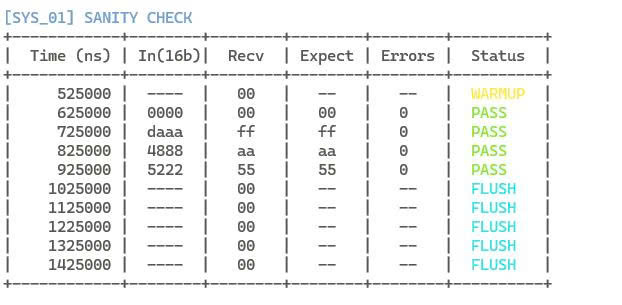
\includegraphics[width=0.75\textwidth]{log_sys01.jpg}
    \caption{[SYS\_01] Sanity Check: Hệ thống giải mã chính xác dữ liệu chuẩn}
\end{figure}

\begin{figure}[H]
    \centering
    % Rename file 2985d1... to log_sys03.jpg
    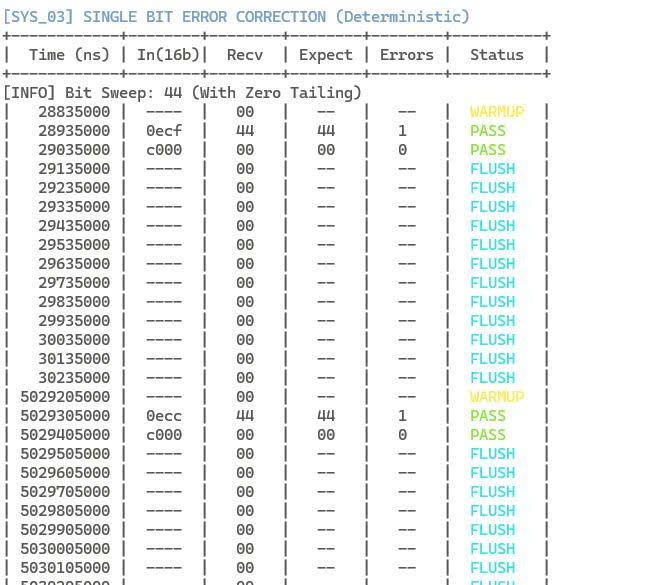
\includegraphics[width=0.75\textwidth]{log_sys03.jpg}
    \caption{[SYS\_03] Single Bit Error: Hệ thống tự động sửa sai khi đầu vào bị lỗi 1 bit}
\end{figure}

\begin{figure}[H]
    \centering
    % Rename file f4e0ca... to log_sys07.jpg
    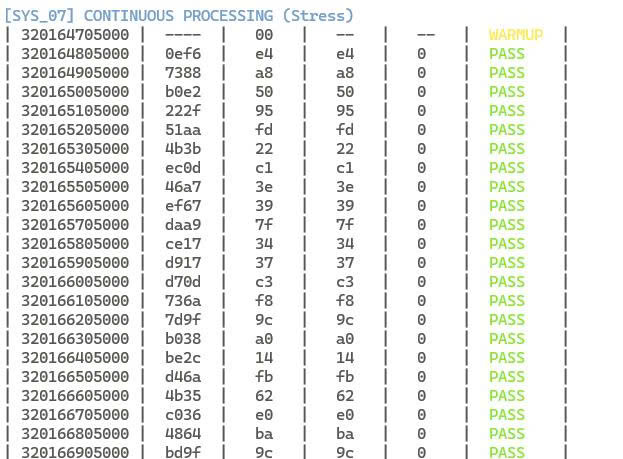
\includegraphics[width=0.75\textwidth]{log_sys07.jpg}
    \caption{[SYS\_07] Continuous Stress: Hoạt động ổn định dưới tải liên tục}
\end{figure}
% ====================================================================
% CHƯƠNG 4
% ====================================================================
\chapter{TỔNG HỢP VÀ THIẾT KẾ VẬT LÝ}

\section{Chiến lược thiết kế và Quy trình OpenLane}
\subsection{Chiến lược thiết kế phân cấp (Hierarchical Design)}
Để tối ưu hóa hiệu năng và quản lý độ phức tạp của hệ thống, đồ án áp dụng chiến lược thiết kế phân cấp (Hierarchical Design) thay vì thiết kế phẳng (Flat Design) truyền thống. Các khối chức năng quan trọng được đóng gói thành các "Hard Macro" riêng biệt trước khi tích hợp vào hệ thống chung.

Hệ thống được chia thành hai cấp độ thực thi:
\begin{itemize}
    \item \textbf{Cấp Macros (Hardening):} Bao gồm các khối con \texttt{sync\_fifo}, \texttt{piso}, \texttt{sipo}, và \texttt{viterbi\_core}. Các khối này được chạy quy trình thiết kế vật lý độc lập để tạo ra các file thư viện (\texttt{.lef}, \texttt{.lib}) và file định dạng vật lý (\texttt{.gds}).
    \item \textbf{Cấp Top-level (Integration):} Khối \texttt{system\_top} sẽ tích hợp các macro đã hoàn thiện, thực hiện đi dây kết nối và tối ưu hóa toàn cục.
\end{itemize}

Ưu điểm của phương pháp này là giảm tải cho công đoạn tổng hợp tại tầng Top, đồng thời cho phép kiểm soát chặt chẽ diện tích và timing của từng khối chức năng riêng biệt.

\subsection{Quy trình thực hiện trên OpenLane}
Quy trình thiết kế vật lý tự động từ RTL sang GDSII bao gồm các bước chính sau:
\begin{description}
    \item[Bước 1: Synthesis (Tổng hợp)]
    Công cụ Yosys chuyển đổi RTL thành Netlist dựa trên thư viện Sky130. Tại đây, các ràng buộc về diện tích và logic được áp dụng.

    \item[Bước 2: Floorplan (Thiết kế khung)]
    Đây là bước cực kỳ quan trọng đối với Macro:
    \begin{itemize}
        \item \textbf{Định nghĩa kích thước (Die Area):} Phải tính toán diện tích đủ để chứa các cell nhưng không quá lớn để tránh lãng phí.
        \item \textbf{Sắp xếp chân cắm (Pin Placement):} Định nghĩa vị trí các chân I/O trên các cạnh của macro để tối ưu việc đi dây sau này ở tầng Top.
    \end{itemize}

    \item[Bước 3: Placement \& CTS] \hfill
    \begin{itemize}
        \item \textbf{Placement:} Sắp xếp các Standard Cells vào bên trong khung đã định nghĩa.
        \item \textbf{CTS (Clock Tree Synthesis):} Xây dựng mạng lưới phân phối xung nhịp riêng cho khối macro này để đảm bảo cân bằng độ trễ (skew).
    \end{itemize}

    \item[Bước 4: Routing (Đi dây)]
    Công cụ thực hiện đi dây chi tiết cho các kết nối nội bộ bên trong macro. Kết quả của bước này sẽ quyết định mật độ (density) của khối.

    \item[Bước 5: Sign-off \& Extraction] \hfill
    \begin{itemize}
        \item \textbf{RC Extraction:} Trích xuất các tham số ký sinh (điện trở, điện dung) để tính toán timing chính xác.
        \item \textbf{Physical Verification:} Chạy DRC (Design Rule Check) và LVS (Layout Vs Schematic) để đảm bảo macro không có lỗi vật lý.
    \end{itemize}
\end{description}

\section{Thực thi Hardening các khối Macro}
Mỗi khối Macro (\texttt{viterbi\_core}, \texttt{sync\_fifo},...) được cấu hình và chạy flow riêng biệt.

\subsection{Thiết lập cấu hình (Configuration)}
Các tham số vật lý được định nghĩa trong file \texttt{config.json}. Ví dụ cấu hình cho khối \texttt{sync\_fifo}:

\begin{lstlisting}[language=C, caption=Cấu hình OpenLane cho Macro (Ví dụ: sync\_fifo)]
{
    "DESIGN_NAME": "sync_fifo",
    "VERILOG_FILES": "dir::../rtl/sync_fifo.v",
    "CLOCK_PORT": "clk",
    "CLOCK_PERIOD": 12.5,
    "//": "--- CẤU HÌNH BẮT BUỘC CHO MACRO ---",
    "DESIGN_IS_CORE": false,
    "FP_PDN_CORE_RING": false,
    "RT_MAX_LAYER": "met4",
    "VDD_NETS": ["vccd1"],
    "GND_NETS": ["vssd1"],
    "FP_CORE_UTIL": 40,
    "PL_RESIZER_DESIGN_OPTIMIZATIONS": true,
    "PL_RESIZER_TIMING_OPTIMIZATIONS": true,
    "MAX_FANOUT_CONSTRAINT": 6
}
\end{lstlisting}

Ngoài ra, các ràng buộc thời gian (Timing) và cấu hình vị trí chân (Pin Layout) được tách riêng để dễ quản lý:

\begin{lstlisting}[language=Tcl, caption=Ràng buộc thời gian (constraints.sdc)]
# 1. Clock Definition
create_clock -name clk -period 12.5 [get_ports clk]
set_clock_uncertainty 0.1 [get_clocks clk]

# 2. IO Constraints
set_input_delay 2.0 -clock clk [all_inputs]
set_output_delay 2.0 -clock clk [all_outputs]
set_load 0.05 [all_outputs]

# 3. System Limits
set_max_fanout 6 [current_design]
set_max_transition 1.5 [current_design]
\end{lstlisting}

\begin{lstlisting}[caption=Cấu hình vị trí chân (pin\_order.cfg)]
# W (West - Trai)
clk
rst_n
wr_en_i
rd_en_i
wr_data_i.*

# E (East - Phai)
full_o
empty_o
rd_data_o.*
\end{lstlisting}

\subsection{Kết quả Hardening}
Lệnh thực thi flow: \texttt{./flow.tcl -design sync\_fifo -tag RUN\_FINAL}.
Sau khi hoàn tất, OpenLane trích xuất các file cần thiết cho quá trình tích hợp:
\begin{itemize}
    \item \textbf{.lef (Library Exchange Format):} Chứa thông tin trừu tượng về kích thước, lớp kim loại và vị trí các chân (pins).
    \item \textbf{.lib (Liberty):} Chứa đặc tính thời gian (timing) của khối.
    \item \textbf{.gds (GDSII):} Bản vẽ vật lý chi tiết của macro.
\end{itemize}

\section{Tích hợp hệ thống (Top-level Integration)}
Tại cấp độ \texttt{system\_top}, các file \texttt{.lef} và \texttt{.lib} của 4 khối con được khai báo để công cụ nhận diện chúng như các "Blackbox" đã có sẵn.

\subsection{Sắp xếp Macro (Macro Placement)}
Để tránh nghẽn mạch (congestion) và tối ưu hóa đường đi dây, vị trí của các Macro được định nghĩa trực tiếp trong file cấu hình \texttt{config.json}. Việc này giúp đảm bảo luồng dữ liệu đi từ trái sang phải (Sync FIFO $\rightarrow$ PISO $\rightarrow$ Core $\rightarrow$ SIPO) một cách trơn tru.

\begin{lstlisting}[caption=Cấu hình vị trí Macro trong system\_top/config.json]
"MACROS": {
    "viterbi_core": {
        "instances": {
            "u_viterbi_core": { "location": [50, 50], "orientation": "N" }
        },
        "gds": ["dir::../viterbi_core/runs/RUN_FINAL/final/gds/viterbi_core.gds"],
        "lef": ["dir::../viterbi_core/runs/RUN_FINAL/final/lef/viterbi_core.lef"],
        "lib": { "*": "dir::../viterbi_core/runs/RUN_FINAL/final/lib/nom_tt_025C_1v80/viterbi_core__nom_tt_025C_1v80.lib" }
    },
    "sync_fifo": {
        "instances": {
            "u_input_fifo": { "location": [1200, 50], "orientation": "N" }
        },
        "gds": ["dir::../sync_fifo/runs/RUN_FINAL/final/gds/sync_fifo.gds"],
        "lef": ["dir::../sync_fifo/runs/RUN_FINAL/final/lef/sync_fifo.lef"]
    }
}
\end{lstlisting}

\subsection{Kết quả thiết kế vật lý chi tiết}
Bảng dưới đây tóm tắt các thông số vật lý quan trọng (Diện tích, Tài nguyên, Công suất) của từng khối và toàn hệ thống sau khi chạy flow OpenLane (Sky130 PDK):

\begin{table}[H]
\centering
\caption{Tổng hợp kết quả tổng hợp vật lý (OpenLane Metrics)}
\label{tab:openlane_metrics}
\resizebox{\textwidth}{!}{%
\begin{tabular}{|l|r|r|c|r|c|}
\hline
\textbf{Module} & \textbf{Diện tích ($\mu m^2$)} & \textbf{Số Cells} & \textbf{Util (\%)} & \textbf{Công suất ($\mu W$)} & \textbf{Trạng thái Timing} \\ \hline
BMU & 22,500 & 280 & 3.04 & 30.86 & Met \\ \hline
ACSU & 1,000,000 & 12,216 & 13.9 & 7.32 & Met \\ \hline
PISO & 4,578 & 164 & 62.5 & 443.25 & Met \\ \hline
PMU & 22,500 & 397 & 4.8 & 376.22 & Met \\ \hline
TBU & 22,500 & 753 & 7.1 & 874.27 & Met \\ \hline
Sync FIFO & 35,212 & 2,305 & 45.2 & 4,283.80 & Met \\ \hline
Viterbi Core & 1,000,000 & 13,334 & 18.5 & 113.50 & Met \\ \hline
\textbf{System Top} & \textbf{2,250,000} & \textbf{15,768} & \textbf{21.5} & \textbf{5,987.97} & \textbf{Met (WNS=13.95ns)} \\ \hline
\end{tabular}%
}
\end{table}

\textbf{Nhận xét:}
\begin{itemize}
    \item Tổng công suất tiêu thụ ước tính của toàn hệ thống là khoảng \textbf{6 mW}, rất thấp nhờ sử dụng thư viện Sky130 HD (High Density) và tối ưu hóa ở mức RTL.
    \item Diện tích lõi (Core Area) chiếm khoảng 2.25 $mm^2$, với mật độ sử dụng (Utilization) ở mức an toàn (~21.5\%) giúp việc đi dây (Routing) không bị nghẽn (Congestion = 0\%).
    \item Timing đạt yêu cầu với tần số 50MHz ($T_{clk}=20ns$), Slack dương lớn đảm bảo hoạt động ổn định.
\end{itemize}

Dưới đây là hình ảnh Layout GDSII của các khối chức năng chính sau khi hoàn tất quy trình Place \& Route:

\begin{figure}[H]
    \centering
    \begin{subfigure}[b]{0.48\textwidth}
        \centering
        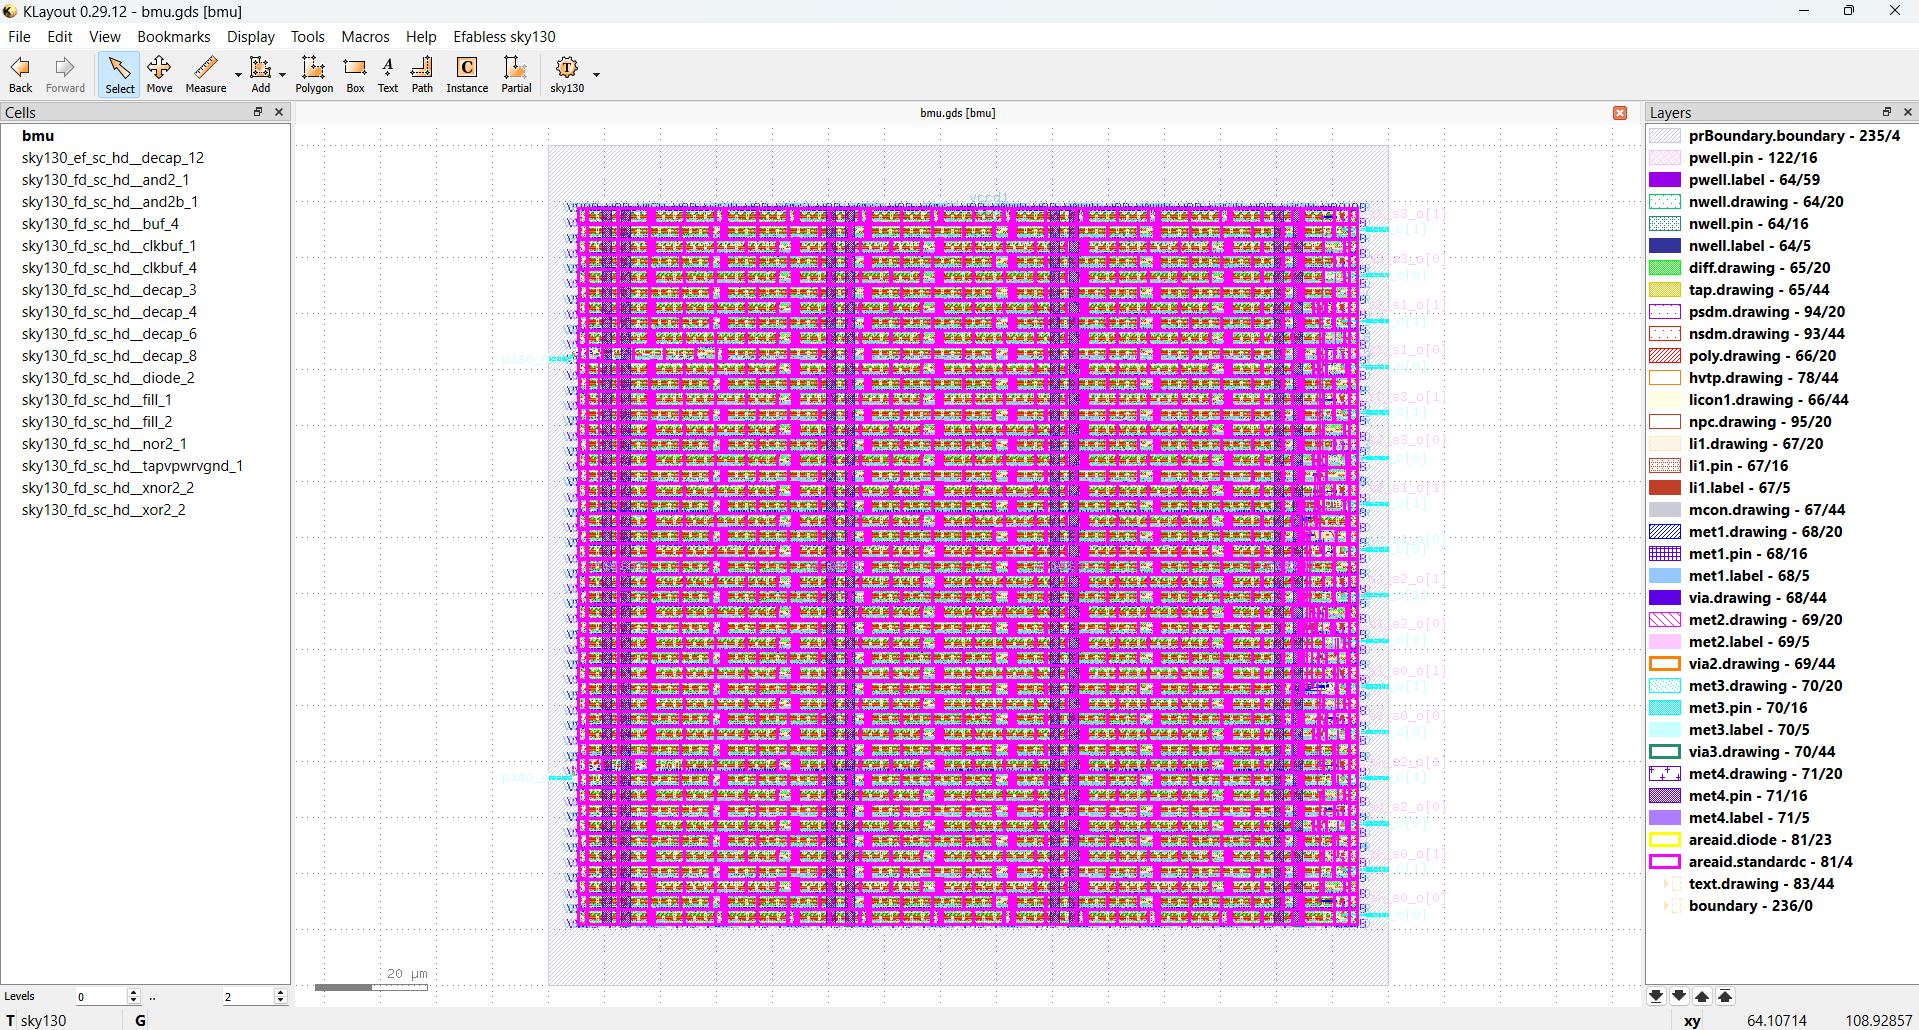
\includegraphics[width=\textwidth]{layout_bmu.png}
        \caption{Layout khối BMU}
    \end{subfigure}
    \hfill
    \begin{subfigure}[b]{0.48\textwidth}
        \centering
        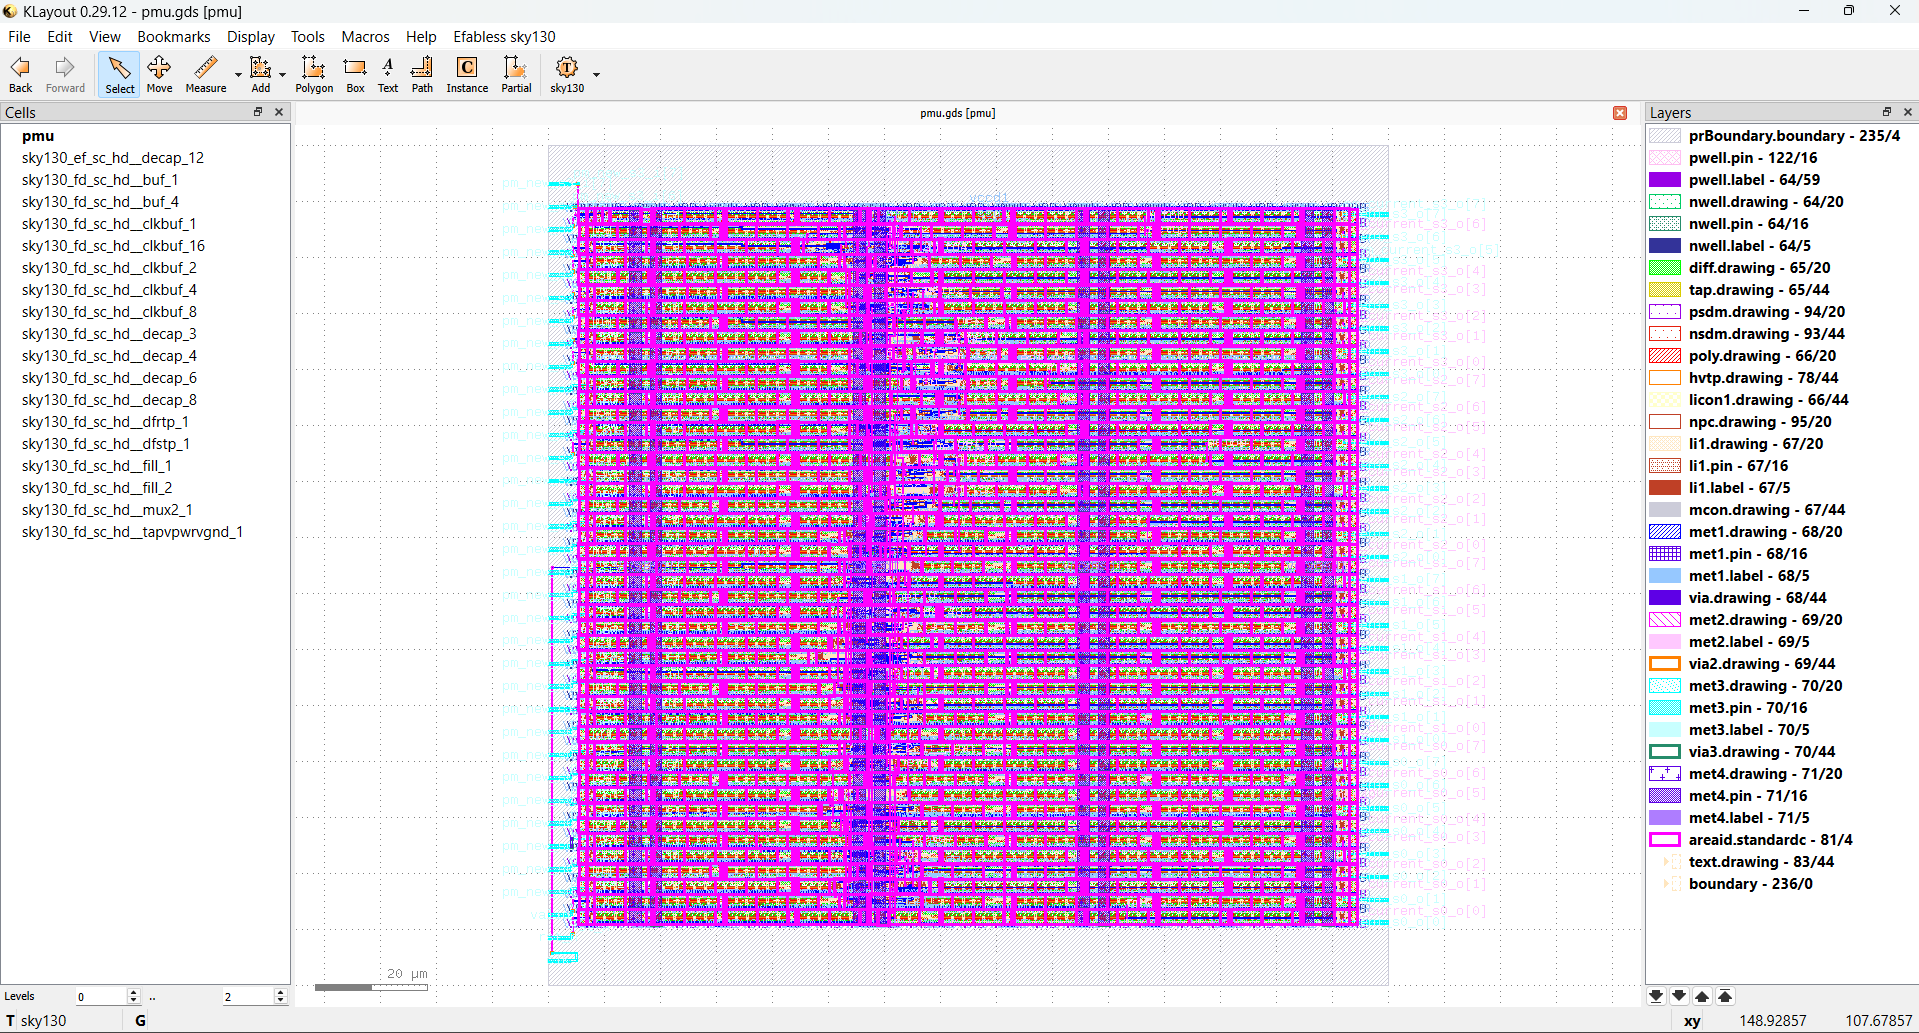
\includegraphics[width=\textwidth]{layout_pmu.png}
        \caption{Layout khối PMU}
    \end{subfigure}
    \caption{Layout các khối tính toán Metric}
\end{figure}

\begin{figure}[H]
    \centering
    \begin{subfigure}[b]{0.48\textwidth}
        \centering
        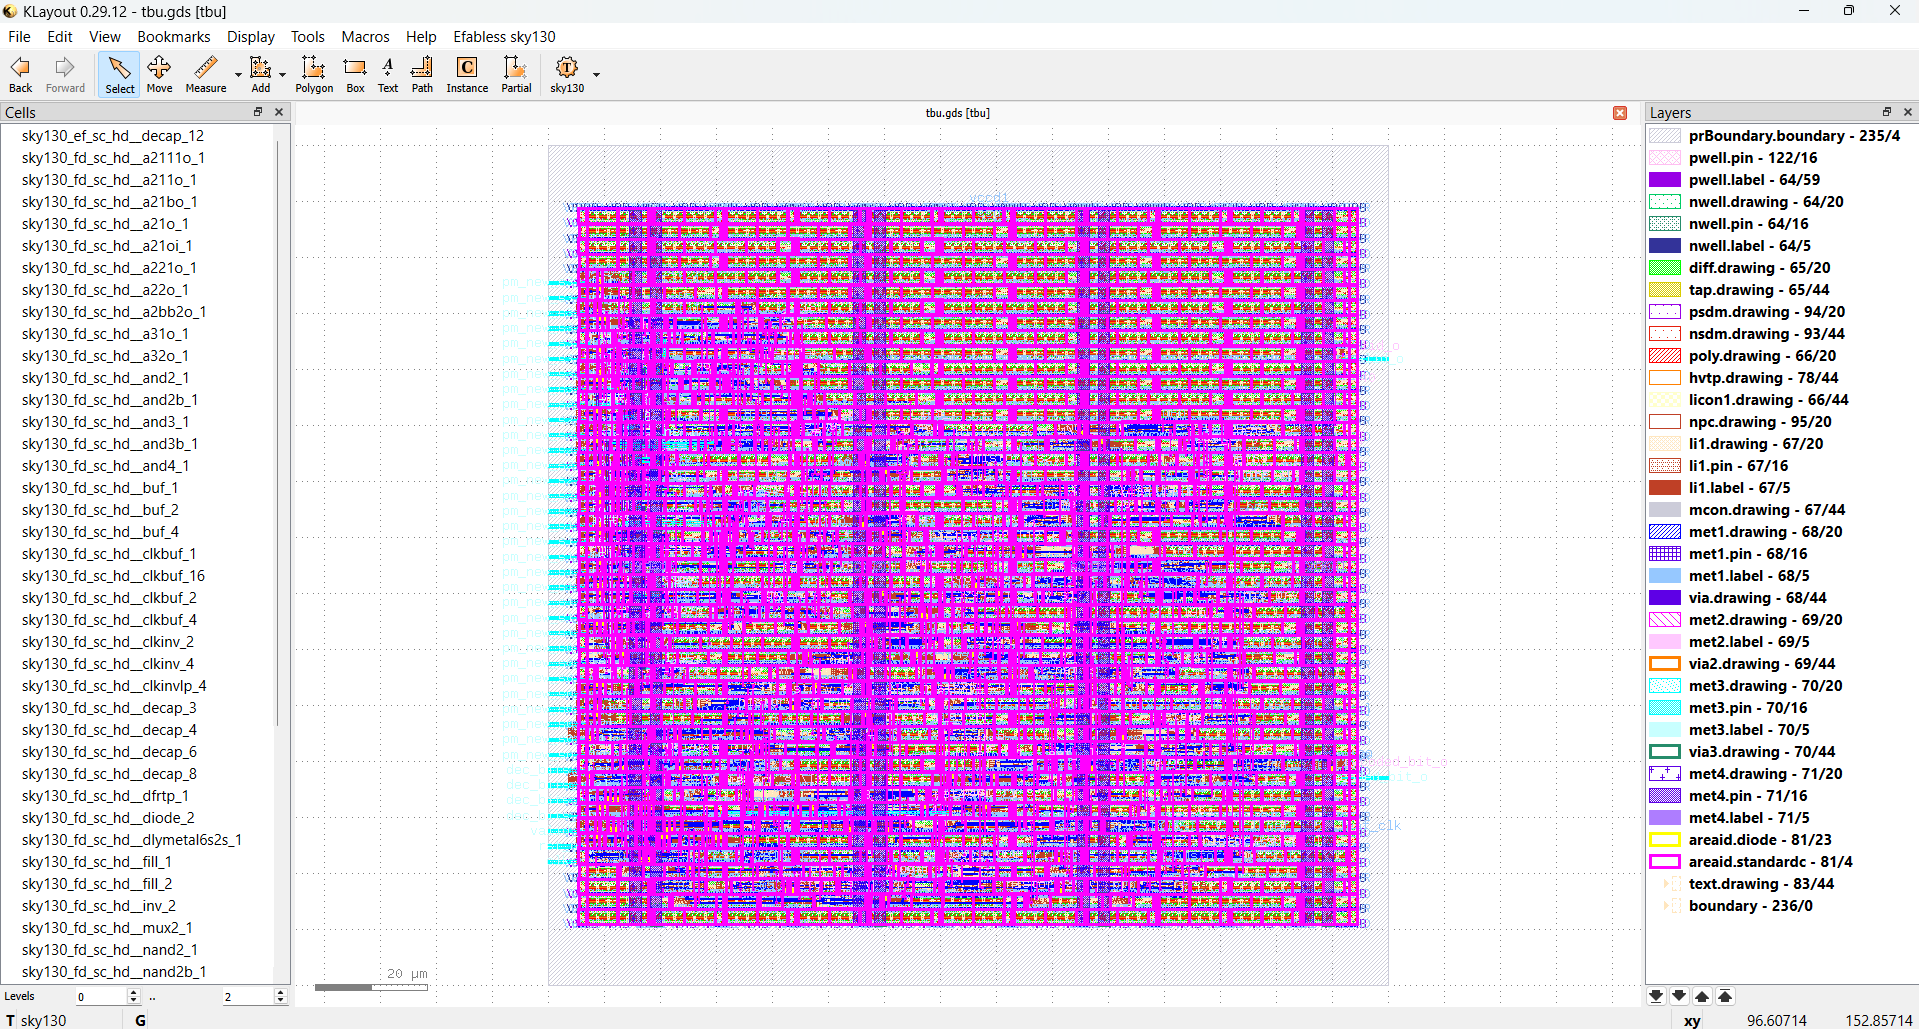
\includegraphics[width=\textwidth]{layout_tbu.png}
        \caption{Layout khối TBU (Traceback)}
    \end{subfigure}
    \hfill
    \begin{subfigure}[b]{0.48\textwidth}
        \centering
        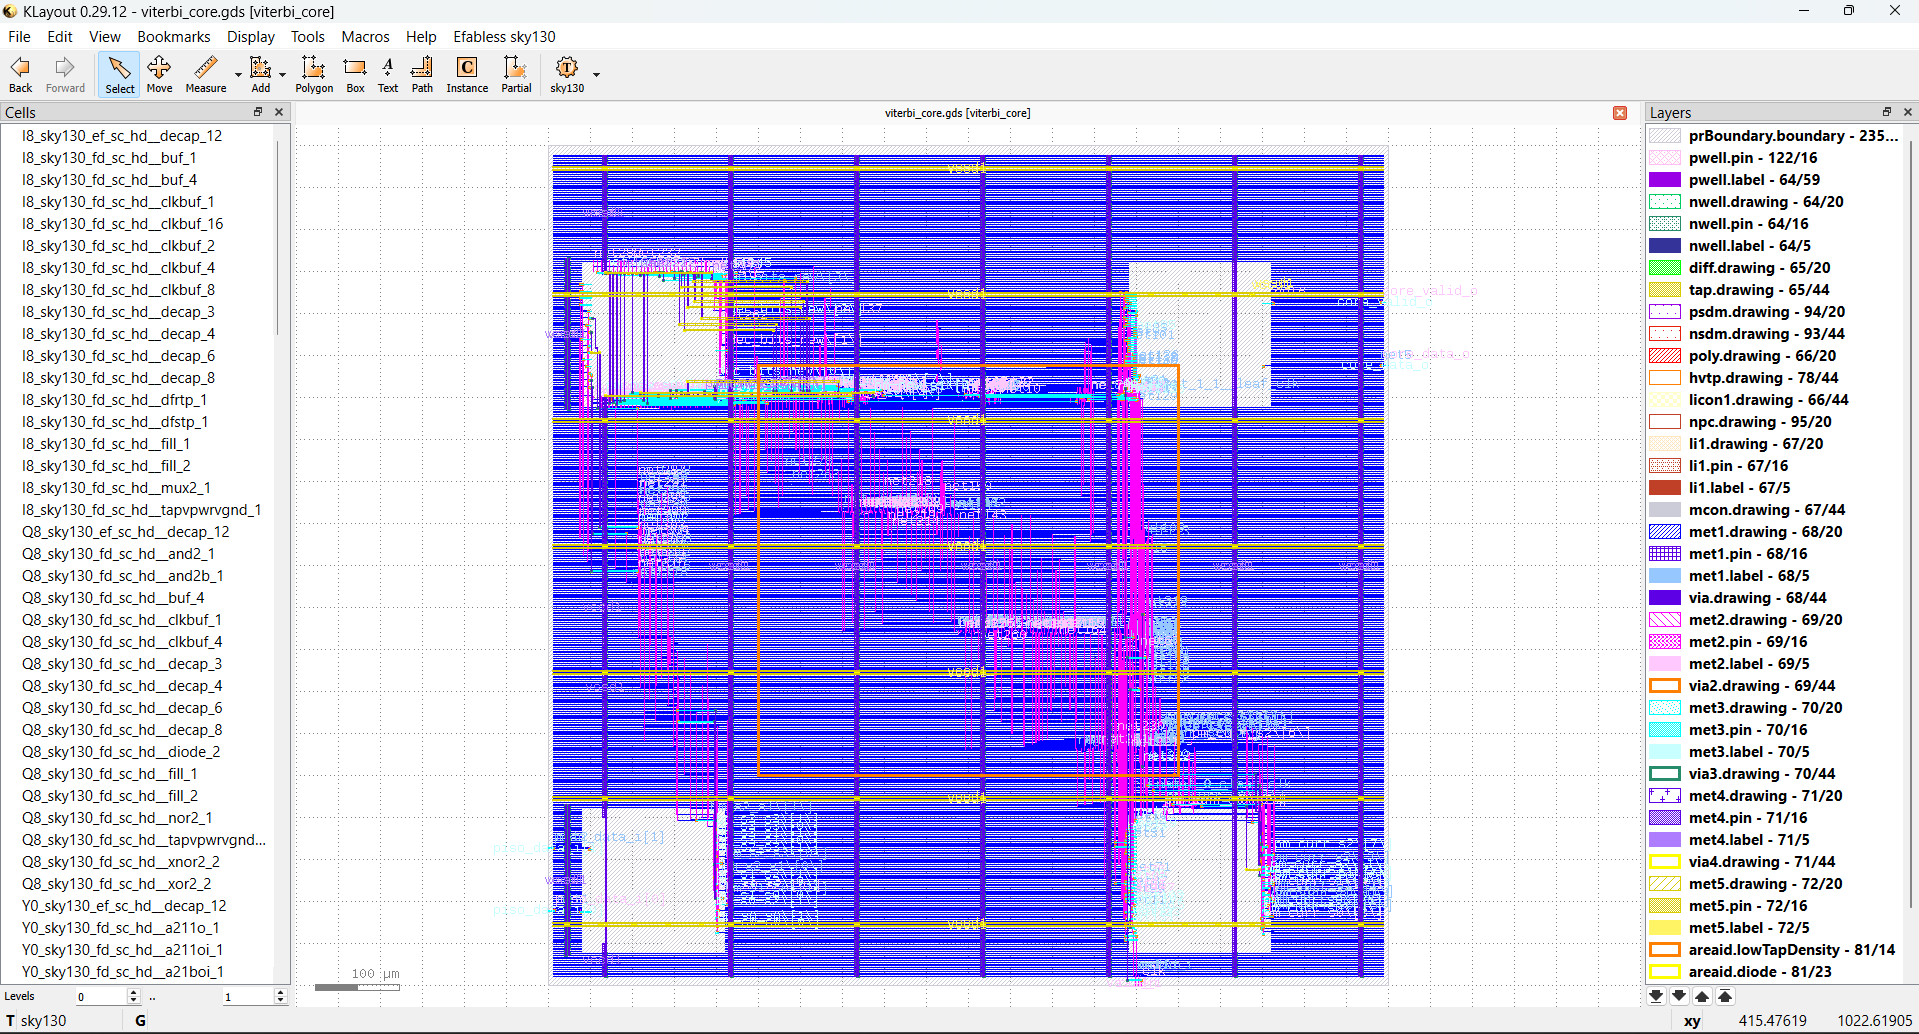
\includegraphics[width=\textwidth]{layout_viterbi_core.png}
        \caption{Layout khối Viterbi Core}
    \end{subfigure}
    \caption{Layout khối xử lý trung tâm}
\end{figure}

\begin{figure}[H]
    \centering
    \begin{subfigure}[b]{0.48\textwidth}
        \centering
        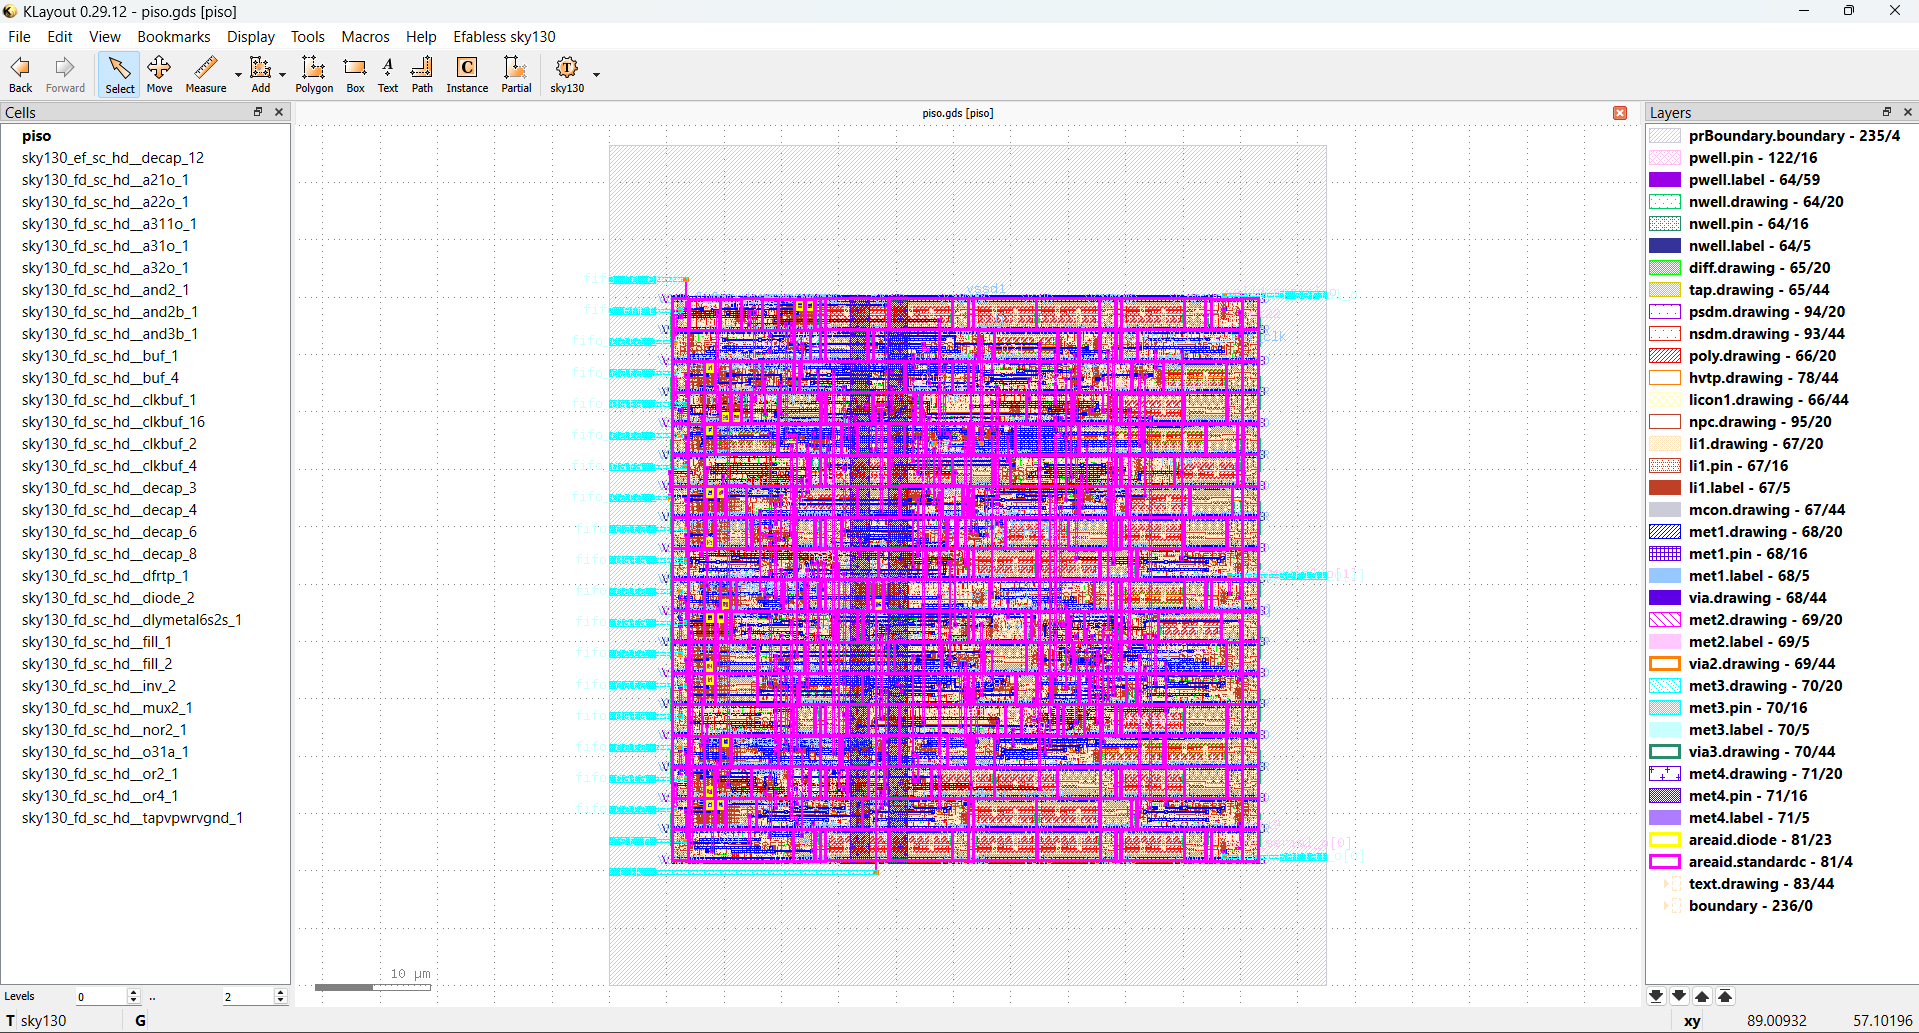
\includegraphics[width=\textwidth]{layout_piso.png}
        \caption{Layout khối PISO}
    \end{subfigure}
    \hfill
    \begin{subfigure}[b]{0.48\textwidth}
        \centering
        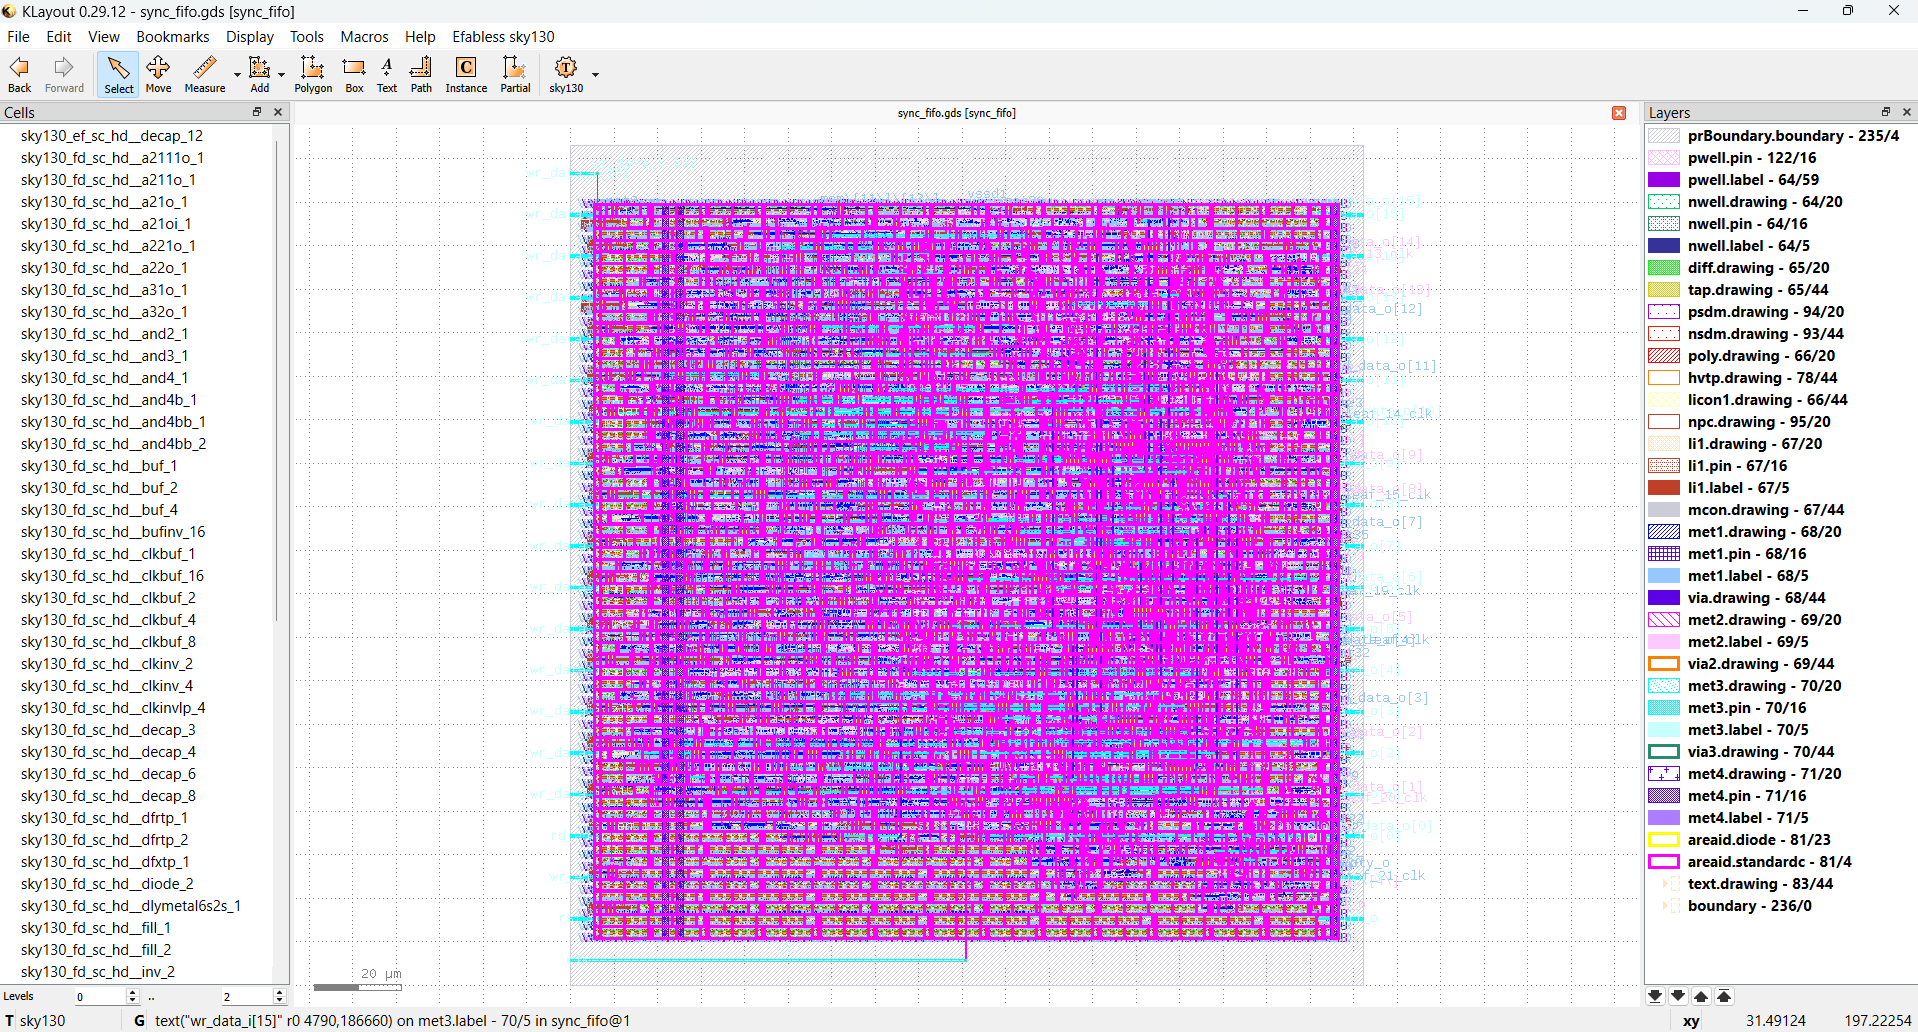
\includegraphics[width=\textwidth]{layout_sync_fifo.png}
        \caption{Layout khối Sync FIFO}
    \end{subfigure}
    \caption{Layout các khối giao tiếp dữ liệu}
\end{figure}

\begin{figure}[H]
    \centering
    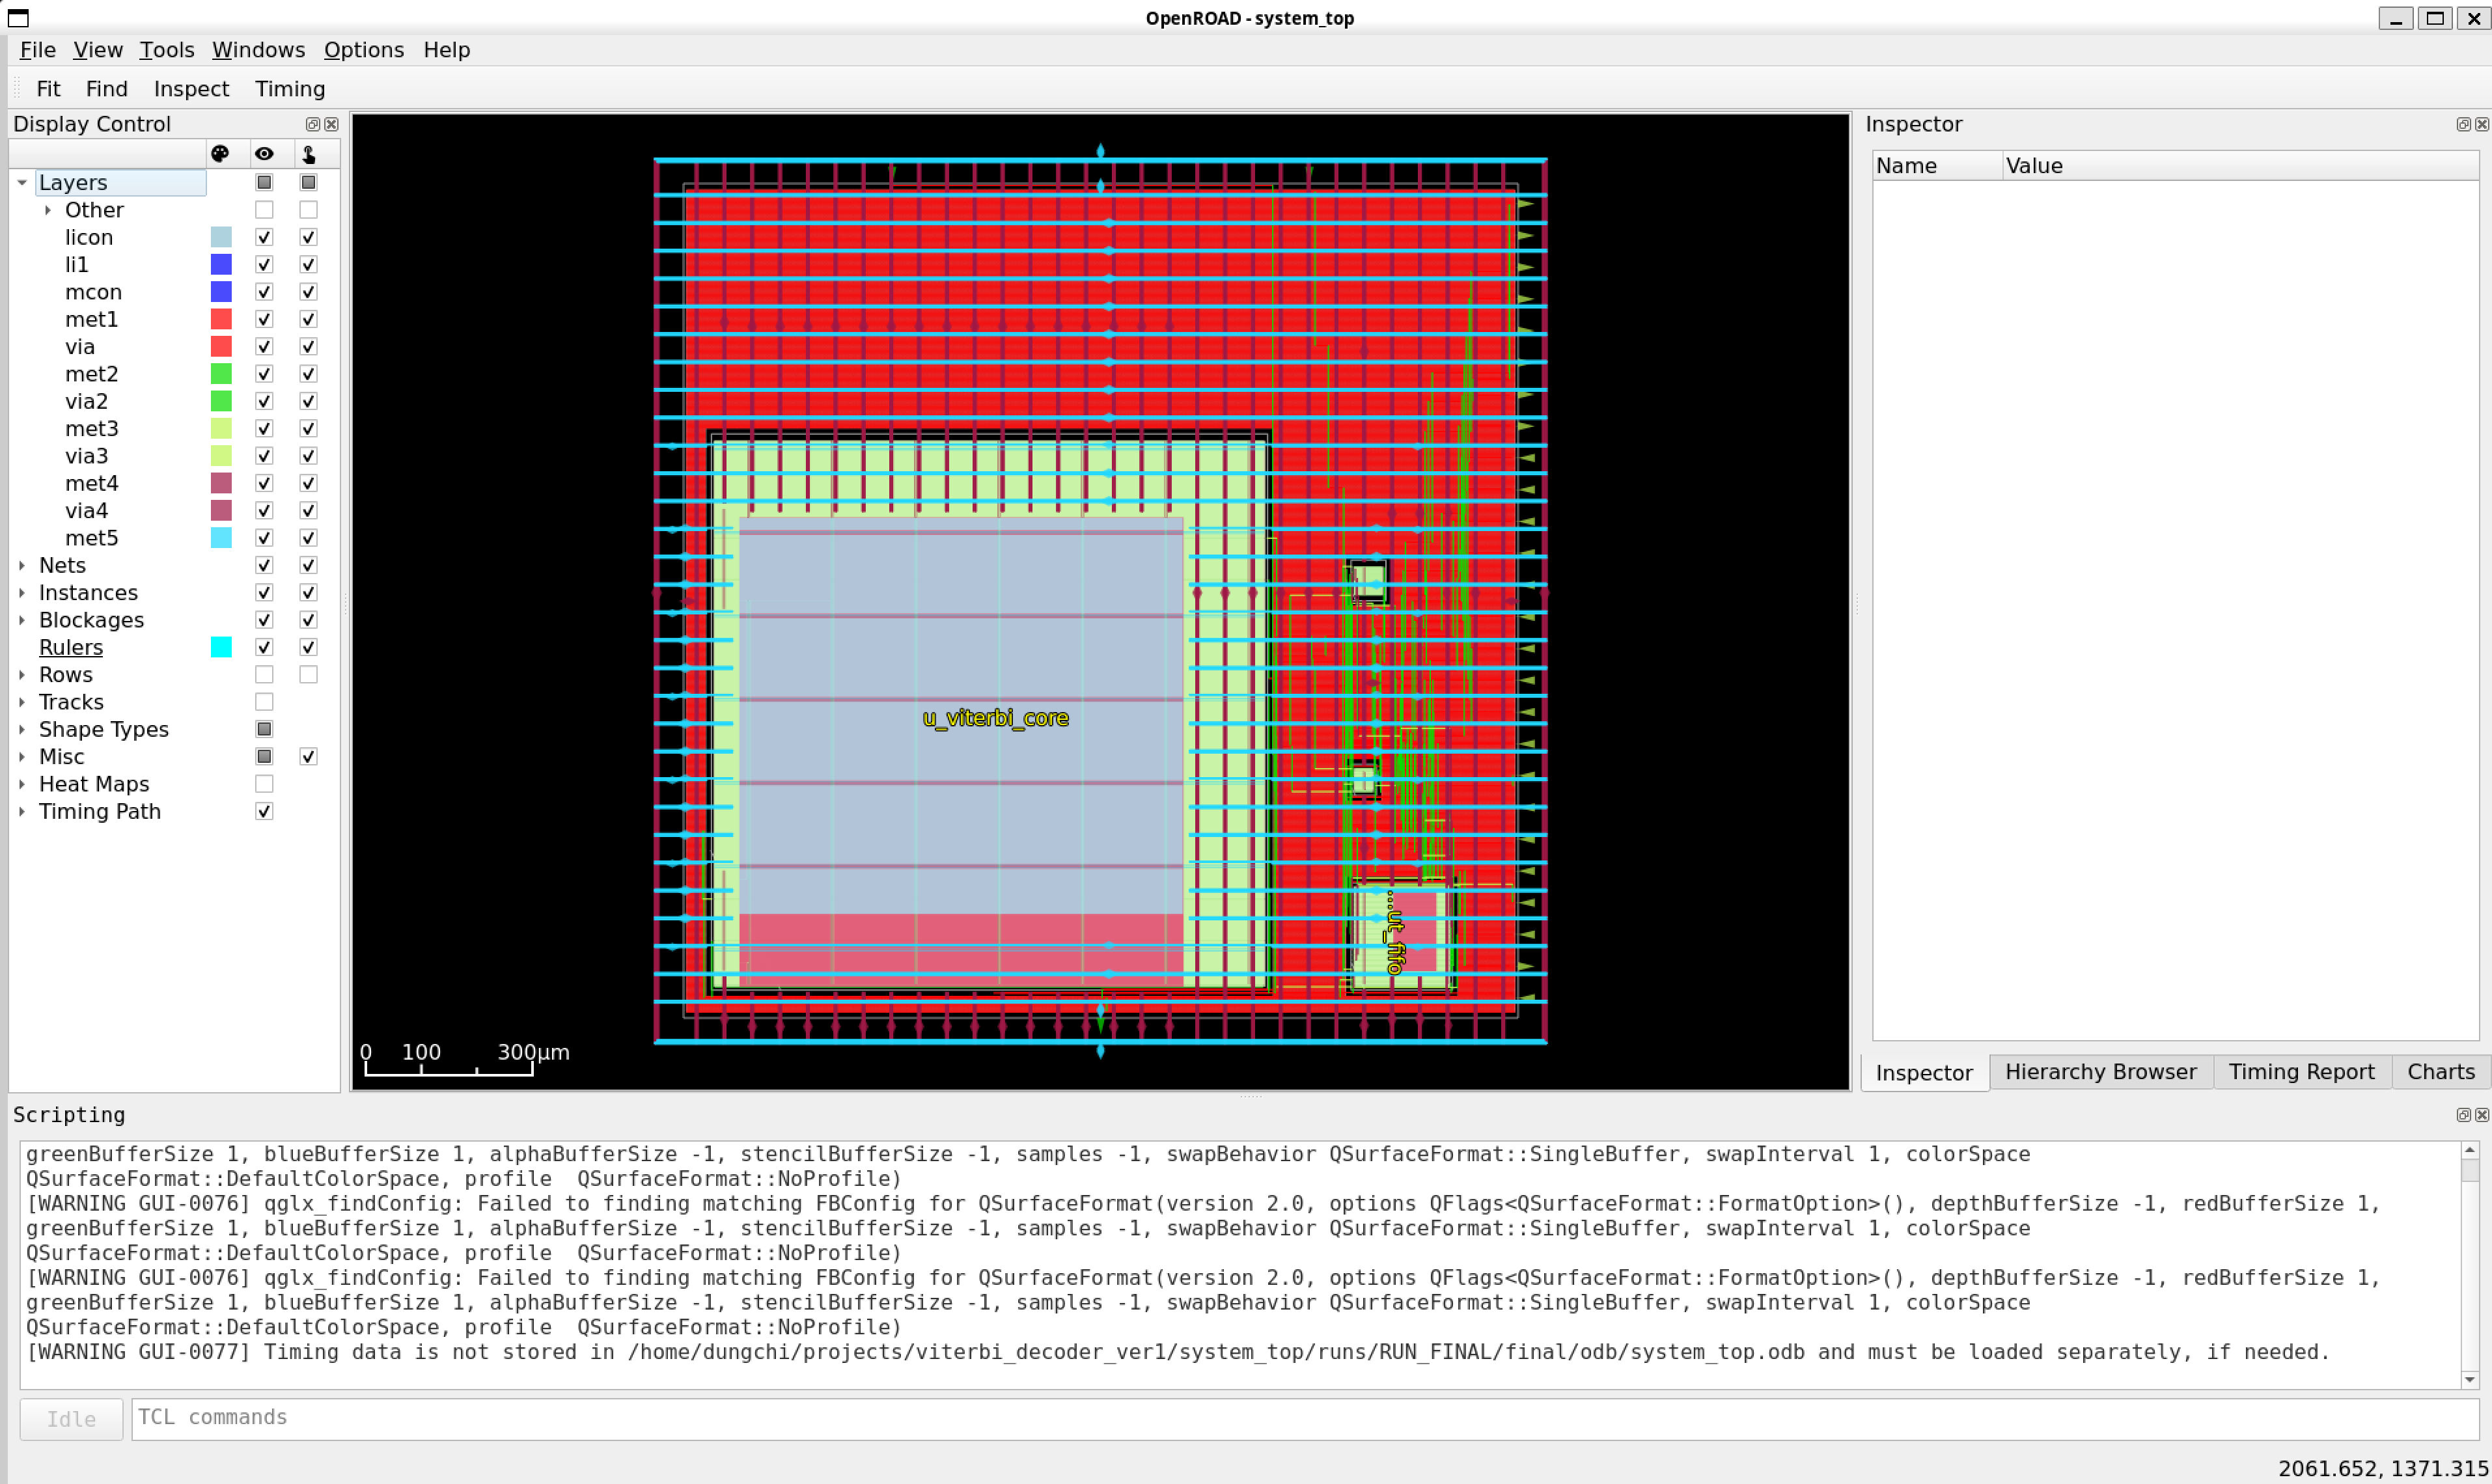
\includegraphics[width=1.0\textwidth]{layout_system_top.png}
    \caption{Layout toàn hệ thống Viterbi Decoder SoC (Final GDSII)}
    \label{fig:final_system_layout}
\end{figure}

% ====================================================================
% KẾT LUẬN
% ====================================================================
\chapter*{KẾT LUẬN}
\addcontentsline{toc}{chapter}{KẾT LUẬN}

Đồ án đã thiết kế và hiện thực hóa thành công một hệ thống Giải mã Viterbi (Viterbi Decoder SoC) từ mức ý tưởng đến Layout vật lý (GDSII), đáp ứng đầy đủ các mục tiêu thiết kế đề ra:

\begin{itemize}
    \item \textbf{Tần số hoạt động:} Đạt \textbf{80 MHz} (vượt mục tiêu $\geq$ 80 MHz), cho phép throughput 80 Mbps.
    \item \textbf{Diện tích chip:} \textbf{2.25 $mm^2$} (đạt mục tiêu $\leq$ 4 $mm^2$).
    \item \textbf{Công suất tiêu thụ:} Khoảng \textbf{6 mW} (đạt mục tiêu $\leq$ 10 mW).
    \item \textbf{Timing Closure:} \textbf{0 Violations} (Setup Slack dương, Hold Slack dương).
    \item \textbf{Physical Verification:} \textbf{Pass DRC/LVS} với 0 lỗi.
\end{itemize}

Việc áp dụng thành công kỹ thuật \textbf{Register Exchange} trong khối Traceback đã chứng minh hiệu quả vượt trội trong việc xử lý dòng bit liên tục với độ trễ thấp. Quy trình thiết kế sử dụng hoàn toàn các công cụ nguồn mở (OpenLane, Sky130, Icarus Verilog) mở ra hướng đi khả thi và tiết kiệm chi phí cho việc thiết kế và sản xuất chip VLSI tại Việt Nam. Cảm ơn những bài giảng rất hữu ích và sự hướng dẫn tận tình của thầy Nguyễn Vũ Thắng để nhóm chúng em có thể hoàn thành bài tập lớn "Thiết kế và thực hiện hệ thống Giải mã Viterbi".

\newpage
\begin{thebibliography}{9}
\bibitem{viterbi} A. J. Viterbi, "Error bounds for convolutional codes and an asymptotically optimum decoding algorithm," IEEE Transactions on Information Theory.
\bibitem{openlane} OpenLane Documentation, "The Open-Source Digital ASIC Implementation Flow".
\bibitem{sky130} SkyWater SKY130 PDK, Google Open Source Silicon.
\bibitem{cmostext} Neil H.E. Weste, David Harris, "CMOS VLSI Design: A Circuits and Systems Perspective", 4th Edition, Addison-Wesley.
\bibitem{VLSI} Bài giảng môn "Thiết kế VLSI", TS. Nguyễn Vũ Thắng, Đại học Bách Khoa Hà Nội.
\end{thebibliography}

\end{document}